\RequirePackage{fix-cm}
\documentclass[smallextended]{svjour3}
\bibliographystyle{spmpsci}      % mathematics and physical sciences
\smartqed  % flush right qed marks, e.g. at end of proof
\usepackage{mathptmx}      % use Times fonts if available on your TeX system
\usepackage{graphicx}
\journalname{Computational Optimization and Applications}

\usepackage{amsmath,enumitem,datetime,xfrac,fix-cm,color,multirow,siunitx}
\usepackage{amssymb,mathtools,stmaryrd,dsfont,tikz}
\usepackage{fullpage}
\usepackage[colorlinks, citecolor=blue, bookmarks=True]{hyperref}
\usetikzlibrary{positioning,trees}
\usepackage{algorithm,algpseudocode}
\graphicspath{{Figures/}}
\DeclareGraphicsExtensions{.pdf,.png}

\let\F\mathds\let\C\mathcal\newcommand{\R}{\F{R}}\newcommand{\A}{\tens{A}}
\newcommand{\norm}[1]{{\left\lVert #1 \right\rVert}}
\newcommand{\Norm}[1]{{\left\vert\kern-0.25ex\left\vert\kern-0.25ex\left\vert #1 \right\vert\kern-0.25ex\right\vert\kern-0.25ex\right\vert}}
\newcommand{\IP}[2]{\left\langle #1,#2 \right\rangle}
\newcommand{\ip}[2]{#1 \vcenter{\hbox{\resizebox{6pt}{!}{\ensuremath\cdot}}} #2}
\newcommand{\op}[1]{\operatorname{#1}}
\newcommand{\splitln}[4]{\begin{cases} #1 & #2 \\ #3 & #4\end{cases}}
\newcommand{\1}{\F{1}}
\DeclareMathOperator{\st}{\;s.t.\;}
\renewcommand{\epsilon}{\varepsilon}\renewcommand{\bar}{\overline}
\renewcommand{\hat}{\widehat}\renewcommand{\tilde}{\widetilde}
\DeclareMathOperator*{\argmin}{argmin}
\DeclareMathOperator{\supp}{supp}
\DeclareMathOperator{\id}{id}
\DeclareMathOperator{\sign}{sign}
\newcommand{\Emin}[1][\varf0]{\inf_{#1\in\F H}\op{E}(#1)}

\newcounter{adaptStepCounter}
\newenvironment{adaptiveStep}{\refstepcounter{adaptStepCounter}}{}

% TODO: get rid of this stuff...
\usepackage{clipboard}\newclipboard{aFEMclipboard}
\usepackage{xstring}
\newcommand*{\varf}[1]{%
	\IfEqCase{#1}{%
		{0}{u}%
		{1}{v}%
		{2}{w}%
	}[u#1]%
}
\newcommand*{\Varf}[1]{%
	\IfEqCase{#1}{%
		{0}{U}%
		{1}{V}%
		{2}{W}%
	}[u#1]%
}
\newcommand*{\spcf}[1]{%
	\IfEqCase{#1}{%
		{0}{\F{U}}%
		{1}{\F{V}}%
		{2}{\F{W}}%
	}[\F{U}#1]%
}
\newcommand*{\vard}[1]{%
	\IfEqCase{#1}{%
		{0}{\varphi}%
		{1}{\psi}%
	}[\varphi #1]%
}
\newcommand*{\varx}[1]{%
	\IfEqCase{#1}{%
		{0}{x}%
		{1}{y}%
		{2}{z}%
		{3}{r}%
	}[x#1]%
}
\newcommand*{\vars}[1]{%
	\IfEqCase{#1}{%
		{0}{\alpha}%
		{1}{\beta}%
		{2}{\gamma}%
		{3}{a}%
		{4}{b}%
		{5}{c}%
	}[k#1]%
}
\newcommand*{\Vars}[1]{%
	\IfEqCase{#1}{%
		{0}{\mathrm{A}}%
		{1}{\mathrm{B}}%
		{2}{\Gamma}%
		{3}{A}%
		{4}{B}%
		{5}{C}%
	}[K#1]%
}
\newcommand{\data}{\eta}
\newcommand{\Domain}{\Omega}\newcommand{\domain}{\omega}
\newcommand{\diam}{\op{diam}}
\newcommand{\meshsize}{h}

% vector forms
\newcommand*{\vvarx}[1]{\vec{\varx{#1}}}
\newcommand*{\vvars}[1]{\vec{\vars{#1}}}
\newcommand*{\vvard}[1]{\vec{\vard{#1}}}

% Macro for tracking changes
\usepackage[normalem]{ulem}\renewcommand{\ULthickness}{1.0pt}
\definecolor{darkgreen}{rgb}{0.0, 0.5, 0.0}
\newcommand{\edit}[2]{{\ifmmode\text{\color{red}\sout{\ensuremath{#1}}}\else {\color{red} \sout{#1}}\fi} {\color{darkgreen} #2}}
%\renewcommand{\edit}[2]{#2}
\newcommand{\todo}[1]{{\color{red}#1}}

\author{Antonin Chambolle \and Robert Tovey }
\institute{A. Chambolle \at
	CEREMADE, CNRS \& Université Paris Dauphine, PSL Research University, Paris \\
	\email{chambolle@ceremade.dauphine.fr}, ORCID: 0000-0002-9465-4659          %  \\
	\and
	R. Tovey \at
	MOKAPLAN, INRIA Paris, Paris \\
	\email{robert.tovey@inria.fr}, ORCID: 0000-0001-5411-2268
}
\title{``FISTA'' in Banach spaces with adaptive discretisations}
\begin{document}
	\maketitle
	
	\begin{abstract}
		FISTA is a popular convex optimisation algorithm which is known to converge at an optimal rate whenever \edit{the optimisation domain}{a minimiser} is contained in a suitable Hilbert space. We propose a modified algorithm where each iteration is performed in a \edit{subspace, and that subspace is allowed to change at every iteration}{subset which is allowed to change at every iteration}. \edit{Analytically, this allows us to guarantee convergence in a Banach space setting}{Sufficient conditions are provided for guaranteed convergence}, although at a reduced rate depending on the conditioning of the specific problem. \edit{Numerically we show that a greedy adaptive choice of discretisation can greatly increase the time and memory efficiency in infinite dimensional Lasso optimisation problems.}{These conditions have a natural interpretation when a minimiser exists in an underlying Banach space. A typical example is the Lasso problem where we provide detailed theoretical and numerical analysis.}
	\end{abstract}
	\keywords{Convex optimization \and Multiscale \and Multigrid \and Sparsity \and Lasso}
	
	\section{Introduction}
	The Fast Iterative Shrinkage-Thresholding Algorithm (FISTA) was proposed by Beck and Teboulle \cite{Beck2009} as an extension of Nesterov's fast gradient method \cite{Nesterov2004} and is now a very popular algorithm for minimising the sum of two convex functions.
	We write this as the problem of computing
	\begin{equation}\label{eq: min F = fD+fC}
		\edit{u^* \in \argmin_{\varf0\in\F H}\op{E}(\varf0)}{\Emin}  \qquad\text{such that}\qquad \op{E}(\varf0)\coloneqq \op{f}(\varf0) + \op{g}(\varf0),
	\end{equation}
	where $\op{f}\colon\F H\to\R$ is a convex differentiable function with $L$-Lipschitz gradient and $\op{g}\colon\F H\to\bar\R$ is a convex function, whose ``proximity operator'' is easy to compute. The iterates of the FISTA algorithm will be denoted $\varf0_n\in\F H$. It has been shown that $\op{E}(\varf0_n) - \edit{\op{E}(u^*)}{\Emin}$ converges at the optimum rate of $n^{-2}$ \cite{Beck2009}, and later (after a small modification) the convergence of the iterates was also shown in a general Hilbert space setting \cite{Chambolle2015}. Many further works have gone on to demonstrate faster practical convergence rates for slightly modified variants of FISTA \cite{Tao2016,Liang2017,Alamo2019}.
	
	The contribution of this work is a modified FISTA algorithm which achieves two key properties:
	\begin{itemize}
		\item we extend the convergence results to the case \edit{$\varf0^*\in\bar{\F H}\setminus\F H$ where $\spcf0\coloneqq \bar{\F H}$ is a Banach space}{where the minimum is not achieved. For example, in Lasso discussed in Section~\ref{sec: Lasso definition} there exists a Banach space $\spcf0\supset\F H$ such that $\Emin = \min_{\varf0\in\spcf0}\op{E}(\varf0)$ is achieved in $\spcf0\setminus\F H$}. The proven rate is slower than the optimal $n^{-2}$, but appears to be quite sharp in numerical examples.
		\item we allow for adaptive discretisation such that $\varf0_n\in\spcf0^n\subset\F H$. With simple guarantees on the rates of convergence, we show analytically that applying our FISTA algorithm with inexact discretisation does not reduce the proven rate of convergence. In the Hilbert space setting this is the original $n^{-2}$ rate. In numerical examples we demonstrate that greedy adaptive discretisation strategies can achieve much greater performance than uniform discretisation, both in measures of time and computer memory requirements.
	\end{itemize}
	There is much overlap between the techniques used in this work and those used in the literature of inexact optimisation, although we believe that our interpretation for \edit{the use outside of Hilbert spaces}{use with un-attained minima} is the key theoretical novelty. Some other works for FISTA-like algorithms include \cite{Jiang2012,Villa2013}. Of particular note, our stability estimate for FISTA  in Theorem~\ref{thm: mini FISTA convergence} is very similar to \cite[Prop 2]{Schmidt2011} and \cite[Prop 3.3]{Aujol2015}. This is then used to analyse the convergence properties in our more general Banach space setting where all sources of inexactness come from subspace approximations. The ideas in \cite{Parpas2017} are similar although in application to the proximal gradient method with an additional smoothing on the functional $\op{g}$. The permitted refinement steps are also more broad in our work.
	
	
	\subsection{Outline}
	This work is organised as follows. Section~\ref{sec: prelims} defines notation and the generic form of our proposed refining FISTA algorithm, Algorithm~\ref{alg: refining FISTA}. The main theoretical contribution of this work is the convergence analysis of Algorithm~\ref{alg: refining FISTA} which is split into two parts: first we outline the proof structure in Section~\ref{sec: recipe}, then we state the specific results in the case of FISTA in Section~\ref{sec: FISTA convergence}. The main results are Theorems~\ref{thm: exponential FISTA convergence}/\ref{thm: stronger exponential FISTA convergence} which extend the convergence of FISTA \edit{to infinite dimensional Banach spaces}{to cases with un-attained minima} with uniform/adaptively chosen subspaces $\spcf0^n$ respectively. 
	
	Section~\ref{sec: general examples} presents some general results for the application of Algorithm~\ref{alg: refining FISTA} \edit{}{in Banach spaces }and Section~\ref{sec: Lasso definition} gives a much more detailed discussion of adaptive refinement for Lasso minimisation. In particular, we describe how to choose efficient refining discretisations to approximate \edit{$\varf0^*$}{$\Emin$}, estimate the convergence of $\op{E}$, and identify the support of \edit{$\varf0^*$}{the minimiser}. The numerical results in Section~\ref{sec: numerics} demonstrate these techniques in four different models demonstrating the apparent sharpness of our convergence rates and the computational efficiency of adaptive discretisations.
	
	
	\section{Definitions and notation}\label{sec: prelims}
	\edit{We consider optimisation of \eqref{eq: min F = fD+fC} over two spaces, the Banach space $(\spcf0,\Norm\cdot)$ and Hilbert space $(\F H,\IP\cdot\cdot,\norm\cdot)$, such that 
	\\\centerline{$\displaystyle \exists\varf0^*\in \spcf0 \quad\st\quad \op{E}(\varf0^*) = \min_{\varf0\in\spcf0}\op{E}(\varf0) = \inf_{\varf0\in\F H}\op{E}(\varf0).$}
	Furthermore, define the translated energy
	\\\centerline{$\displaystyle \op{E}_0\colon\spcf0\cup\F H\to \R,\qquad \op{E}_0(\varf0) \coloneqq \op{E}(\varf0)-\op{E}(\varf0^*).$}
	Note that the value of $\op{E}_0$ is uniquely defined, even if $\varf0^*$ may not be.%
	\\}{%
	We consider optimisation of \eqref{eq: min F = fD+fC} over a Hilbert space $(\F H,\IP\cdot\cdot,\norm\cdot)$ with the translated energy
	\begin{equation}
		\op{E}_0\colon\F H\to \R,\qquad \op{E}_0(\varf0) \coloneqq \op{E}(\varf0)-\Emin[\tilde{\varf0}].
	\end{equation}
	}
	
	The proposed generalised FISTA algorithm is stated in Algorithm~\ref{alg: refining FISTA} for an arbitrary choice of \edit{refining subspaces}{closed convex subsets} $\spcf0^n\subset \edit{\spcf0\cap}{}\F H$ for $n=0,1,\ldots$. The only difference \edit{}{from standard FISTA }is that on iteration $n$, all computations are performed in the \edit{subspace}{subset} $\spcf0^n$. If $\spcf0^n\edit{=\spcf0}{}=\F H$ then we recover the \edit{standard FISTA}{original} algorithm.
	
	Without loss of generality we will assume $L=1$, i.e. $\nabla\op{f}$ is 1-Lipschitz. To get the general statement of any of the results which follow, replace $\op{E}$ with $\frac{\op{E}}{L}$.\edit{ A more important distinction is to say that the properties of $\op{f}$ and $\op{g}$ are stated with respect to the Hilbert norm.}{} In particular,
	\begin{equation}
		\norm{\nabla\op{f}(\varf0)- \nabla\op{f}(\varf1)} \leq \norm{\varf0-\varf1}
	\end{equation}
	for all $\varf0,\varf1\in\F H$ and $\op{g}$ is called `simple' if \edit{}{it is proper, convex, weakly lower-semicontinuous, and}
	\begin{equation}
		\argmin_{\varf0\in\tilde{\spcf0}}\tfrac12\norm{\varf0-\varf1}^2 + \op{g}(\varf0)
	\end{equation}
	is exactly computable for all $\varf1\in\F H$ and all $\tilde{\spcf0}\in\{\spcf0^n\}_{n=0}^\infty$. \edit{}{Note in particular we need the argmin to be non-empty. For this we will assume $\spcf0^n$ are locally compact, for example finite dimensional.}
	
	One defining property of the FISTA algorithm is an appropriate choice of inertia, dictated by $t_n$. In particular, we will say that $(t_n)_{n=0}^\infty$ is a \emph{FISTA stepsize} if
	\begin{equation}\label{def: t_n and rho_n}
		t_0 = 1, \qquad t_n \geq 1, \qquad \text{and}\qquad \rho_n \coloneqq t_n^2 - t_{n+1}^2 + t_{n+1} \geq 0\qquad \text{ for all }n=0,1,\ldots.
	\end{equation}
	
	\edit{Finally we introduce the concept of an orthogonal projection in the setting of this work. For a subspace $\spcf0^n\subset\spcf0\cap\F H$ we define the orthogonal projection $\tens{\Pi}_n\colon (\spcf0^n)^*\to \spcf0^n$ to be any extension of the function such that 
	\\\centerline{$\IP{\tens{\Pi}_n\varf0}{\varf1} = \IP{\varf0}{\varf1} \text{ for all } \varf0\in(\spcf0^n)^*, \ \varf1\in\spcf0^n.$}
	This definition is non-standard as we view $(\spcf0^n)^*$ embedded in $\spcf0$. Note that $\spcf0^n\subset\F H$ implies that $(\spcf0^n)^*\supset\F H$, therefore $\tens{\Pi}_n$ is an extension of the classical orthogonal projection. It is convenient to allow an extension here because $\spcf0$ may be bigger than $\F H$, $(\spcf0^n)^*$ is the largest space such that $\tens{\Pi}_n$ is sufficiently well-defined. Beyond this, the Hahn-Banach theorem may allow the domain of $\tens{\Pi}_n$ to be extended further, but the definition is no longer unique. For example, in 1D the value of $\IP{\delta_0}{\frac{1}{\sqrt[4]{\varx0}}}$ is not well-defined, but the value of $\IP{\delta_0}{\1_{[0,1]}}$ can be chosen to be consistent with some sequence of molifiers. To account for this possibility, we shall state that the domain of $\tens{\Pi}_n$ is $\bar{(\spcf0^n)^*}$, with the closure computed in an appropriate topology dictated by $\Norm\cdot$.}{}
	
	The precise constants associated to a given rate are given in the statements of the theorems but, for convenience, are otherwise omitted from the text. For sequences $(a_n)_{n=1}^\infty$,$(b_n)_{n=1}^\infty$ we will use the notation:
	\begin{align*}
		a_n \lesssim b_n \qquad &\iff \qquad \exists C,N>0 \st a_n \leq C b_n \text{ for all } n>N,
		\\ a_n \simeq b_n \qquad &\iff \qquad a_n\lesssim b_n \lesssim a_n.
	\end{align*}
	\edit{}{For $n\in\F N$ we use the abbreviation $[n] = \{1,2,\ldots,n\}$. When the subdifferential of $\op{E}$ is set-valued, we will use the short-hand
	\begin{equation}
		\Norm{\partial\op{E}(\varf0)} \coloneqq \inf_{\varf1\in\partial\op{E}(\varf0)}\Norm{\varf1}
	\end{equation}
	for any specified norm $\Norm\cdot$.}
	
	\begin{algorithm}\caption{Refining \edit{subspace}{subset} FISTA}\label{alg: refining FISTA}
		\centering
		\begin{algorithmic}[1]
			\State Choose $(\spcf0^n)_{n\in\F N}$, $\varf0_0\in \spcf0^0$ and some FISTA stepsize choice $(t_n)_{n\in\F N}$
			\State $\varf1_0\gets \varf0_0, n\gets0$
			\Repeat
			\State $\bar{\varf0}_n \gets (1-\tfrac{1}{t_n})\varf0_n + \tfrac{1}{t_n}\varf1_n$
			\State $\displaystyle \varf0_{n+1} \gets \argmin_{\varf0\in \spcf0^{n+1}} \tfrac12\norm{\varf0-\bar{\varf0}_n+\nabla \op{f}(\bar{\varf0}_n)}^2+\op{g}(\varf0)$ \Comment{Only modification, $\spcf0^{n+1}\subset \spcf0$}
			\State $\varf1_{n+1} \gets (1-t_n)\varf0_n + t_n\varf0_{n+1}$
			\State $n\gets n+1$
			\Until{converged}
		\end{algorithmic}
	\end{algorithm}
	
	
	\section{General proof recipe}\label{sec: recipe}
	In this section we give an intuitive outline of the full proof for convergence of Algorithm~\ref{alg: refining FISTA} before giving formal theorems and proofs in the next section. First we recall the classical FISTA convergence guarantee given by \cite[\edit{Theorem 2}{Thm 3.1}]{Chambolle2015}:
	\begin{equation}\label{eq: classical FISTA}
		t_N^2\op{E}_0(\varf0_N) + \sum^{N-1}_{n=1}\rho_n\op{E}_0(\varf0_n) + \tfrac12\norm{\varf1_N-\varf0^*}^2 \leq \tfrac12\norm{\varf0_0-\varf0^*}^2
	\end{equation}
	for some FISTA stepsize choice $t_N\simeq N$ and $\rho_n\geq0$.
	
	\paragraph{Step 1: Quantifying the stability}
	\begin{adaptiveStep}\label{step: step 1 stability}
		The first step is to generalise \eqref{eq: classical FISTA} to account for the adapting \edit{subspaces}{subsets} $\spcf0^n$. In the notation of Algorithm~\ref{alg: refining FISTA}, Theorem~\ref{thm: mini FISTA convergence} shows that 
		\begin{equation}\label{eq: mini FISTA convergence}
			t_N^2\op{E}_0(\varf0_N) + \sum_{n=1}^{N-1}\rho_n \op{E}_0(\varf0_n) + \tfrac12\norm{\varf1_N-\varf2_N}^2 \leq \tfrac12\norm{\varf0_0-\varf2_0}^2 +\tfrac{\norm{\varf2_N}^2-\norm{\varf2_0}^2}2 
			+ \sum^N_{n=1} t_n\op{E}_0(\varf2_n) + \IP{\varf1_{n-1}}{\varf2_{n-1}-\varf2_n}
		\end{equation}
		for any $\varf2_n \in \argmin_{\varf0\in\spcf0^n}\op{E}(\varf0)$. The similarities to \eqref{eq: classical FISTA} are clear. If $\spcf0^n=\edit{\spcf0}{\F H}$, then we have $\varf2_n=\edit{\varf0^*}{\varf2_0\in\argmin_{\varf0\in\F H}\op{E}(\varf0)}$ and the two estimates agree. These extra terms quantify the robustness to changing of discretisation.
	\end{adaptiveStep}
	
	
	\paragraph{Step 2: Quantifying the scaling properties}
	\begin{adaptiveStep}\label{step: step 2 smoothness}
		To show that the extra terms in \eqref{eq: mini FISTA convergence} are small, we need to quantify the approximation properties of $\spcf0^n$. To do so, we construct a secondary sequence $n_0 < n_1 < \ldots$ and constants $\vars3_{\Varf0},\vars3_{\op{E}}\geq1$ such that for each $k\in\F N$
		\begin{equation}
			n\leq n_k \implies \norm{\varf2_n} \lesssim \vars3_{\Varf0}^k, \qquad n\geq n_k \implies \op{E}_0(\varf2_n) \lesssim \vars3_{\op{E}}^{-k}.
		\end{equation}
		The choice of exponential scaling is very natural if we consider the $\spcf0^n$ to be the subspace of functions discretised on a uniform mesh. If that mesh sequentially refined, then the resolution of the mesh will be of order $h^k$ after $k$ refinements and for some $h<1$. The integer $n_k$ should then be the time when the mesh has refined $k$ times.\edit{}{ Another canonical choice would be $\spcf0^n=\{\varf0\in\F H\st \norm{\varf0}\leq \vars3_{\Varf0}^k\}$. The exponential scaling is less natural, but leads to better convergence guarantees.}
		
		\edit{The value of $\vars3_{\Varf0}$ is dictated by the smoothness of the norm of $\spcf0$ with respect to that of $\F H$. If $\norm{\varf0^*}<\infty$, then the value is $\vars3_{\Varf0}=1$, otherwise there is some damage to the rate of convergence generated by this factor. On the other hand, the value of $\vars3_{\op{E}}$ is dictated by the smoothness of $\op{E}$ at the point $\varf0^*$.}{Suppose $\F H$ is contained in a Banach space $(\spcf0,\Norm\cdot)$ such that $\Norm{\varf2_n}\lesssim 1$, then $\vars3_{\Varf0}$ reflects the smoothness between the two norms. If $\vars3_{\Varf0}>1$, then we cannot guarantee the original $n^{-2}$ rate of convergence. On the other hand, the value of $\vars3_{\op{E}}$ is dictated by the smoothness of $\op{E}$ (measured in $\Norm\cdot$) near minimisers.} %
		If an efficient basis is used, then $\vars3_{\op{E}}$ is large. The trade-off between $\vars3_{\op{E}}$ and $\vars3_{\Varf0}$ dictates the final convergence rate of the algorithm.
	\end{adaptiveStep}
	
	\paragraph{Step 3: Generalising the convergence bound}
	\begin{adaptiveStep}\label{step: step 3 convergence bound}
		In this step we combine the FISTA stability estimate with the \edit{subspace}{subset} approximation guarantees to provide a sharper estimate of stability with respect to the parameters $\vars3_{\op{E}}$ and $\vars3_{\Varf0}$. For example, if $\spcf0^n$ is of the form 
		$$ \spcf0^{n_k} = \spcf0^{n_k+1} = \ldots = \spcf0^{n_{k+1}-1},$$
		then many terms on the right-hand side of \eqref{eq: mini FISTA convergence} telescope to 0. The result of this is presented in Lemma~\ref{thm: mini exponential FISTA convergence} but the moral is that the stability error in \eqref{eq: mini FISTA convergence} should scale in proportion to the $k$ (related to the resolution) rather than the total number of iterations $N$.
	\end{adaptiveStep}
	
	\paragraph{Step 4: Sufficiently fast refinement}
	\begin{adaptiveStep}\label{step: step 4 sufficiently fast}
		In Step~\ref{step: step 3 convergence bound} we developed a convergence bound, now we wish to show that it is only worse than the classical \eqref{eq: classical FISTA} by a constant factor. In particular, it is equivalent to run Algorithm~\ref{alg: refining FISTA} for $N$ iterations or the classical FISTA algorithm for $N$ iterations on the fixed \edit{subspace}{subset} $\spcf0^N$. The estimate from \eqref{eq: classical FISTA} provides the estimate $N^2\op{E}_0(\varf0_N)\lesssim \norm{\varf0_0-\varf2_N}^2 = O(\vars3_{\Varf0}^{2K})$ for $N\leq n_K$. Lemma~\ref{thm: sufficiently fast} shows that Algorithm~\ref{alg: refining FISTA} can achieve the same order of approximation, so long as $\spcf0^n$ refine sufficiently quickly, i.e. $n_k$ are sufficiently small.
	\end{adaptiveStep}
	
	\paragraph{Step 5: Sufficiently slow refinement}
	\begin{adaptiveStep}\label{step: step 5 sufficiently slow}
		The result of Step~\ref{step: step 4 sufficiently fast} is sufficient to prove convergence, but not yet a rate. If the \edit{subspaces refine}{subsets grow} too quickly, then the influence of \edit{$\norm{\varf0^*}=\infty$}{$\norm{\varf0_n}\to\infty$} will slow the rate of convergence. If the resolution is too coarse then we are overfitting to the discretised problem, but if the resolution is too fine then convergence of the energy is slow. Lemma~\ref{thm: sufficiently slow} balances these two factors in an optimal way for Algorithm~\ref{alg: refining FISTA} resulting in a convergence rate of 
		$$ \op{E}_0(\varf0_N) \lesssim \frac{\vars3_{\Varf0}^{2K}}{N^2} \lesssim \frac{N^{2\kappa}}{N^2}$$
		for all $N\in\F N$, some $\kappa\in[0,1)$ depending on $\vars3_{\Varf0},\vars3_{\op{E}}$. In particular, if \edit{$\varf0^*\in\F H$}{the minimum is attained in $\F H$,} then we recover the classical rate with $\kappa=0$.
	\end{adaptiveStep}
	
	\paragraph{Step 6: Adaptivity}
	\begin{adaptiveStep}\label{step: step 6 adaptivity}
		Up to this point we have implicitly focused on the case where $\spcf0^n$ (and $n_k$) are chosen a priori. Here we emphasise some of the challenges which are faced when extending results to allow for greedy adaptivity.
		
		Spatial adaptivity is robust, so long as the scaling properties of Step~\ref{step: step 2 smoothness} are satisfied. The only other constraint is to ensure that the partial telescoping of Step~\ref{step: step 3 convergence bound} still holds. Lemma~\ref{thm: mini exponential FISTA convergence} shows that a sufficient condition is
		$$\edit{}{\varf0_{n_k-1}\in}\spcf0^{n_k}\subset\spcf0^{n_k+1}\subset\ldots\subset\spcf0^{n_{k+1}-1}.$$
		Convergence is most stable if the approximation spaces $\spcf0^n$ satisfy a monotone inclusion, breaking the monotonicity requires more care.
		
		Adaptively choosing the time of refinement is more challenging due to the non-descent property of FISTA. The idea is that $\spcf0^n$ should be refined as soon as the value $\op{E}(\varf0_n)$ is sufficiently close to $\op{E}(\varf2_n)$. This is analysed in Theorem~\ref{thm: stronger exponential FISTA convergence} (sufficient conditions in Lemma~\ref{thm: practical refinement criteria}) which shows convergence results of the form
		$$ \min_{n\leq N}\op{E}_0(\varf0_n) \lesssim \frac{N^{2\kappa}}{N^2}$$
		for all $N\in\F N$, with the same $\kappa\in[0,1)$ from Step~\ref{step: step 5 sufficiently slow}. The penalty for accelerating the refinement time is a potential loss of stability in $\op{E}(\varf0_n)$, however, the asymptotic rate is equivalent and this behaviour has not been seen in numerical experiments.
	\end{adaptiveStep}
	
	\section{Proof of convergence}\label{sec: FISTA convergence}
	In this section we follow the recipe motivated in Section~\ref{sec: recipe} to prove convergence of two variants of Algorithm~\ref{alg: refining FISTA}. Each of the main theorems and lemmas will be stated with a sketch proof in this section. The details of the proofs are either trivial or very technical and are therefore placed in Section~\ref{app: FISTA convergence} to preserve the flow of the argument.
	
	\subsection{Computing the convergence bound}
	For Step~\ref{step: step 1 stability} of Section~\ref{sec: recipe} we look to replicate the classical bound of the form in \eqref{eq: classical FISTA} for Algorithm~\ref{alg: refining FISTA}. The proofs in this step follow the classical arguments \cite{Beck2009,Chambolle2015} very closely. 
	\edit{}{Throughout this section we consider a sequence $(\spcf0^n)_{n\in\F N}$ which generate the iterates $(\varf0_n)_{n\in\F N}$ in Algorithm~\ref{alg: refining FISTA} satisfying
	\begin{equation}\label{eq: refining subspace definition}
		\varf0^{n-1}\in\spcf0^n\subset\F H \quad\text{are closed, convex, locally compact subsets for all }\quad n\in\F N.
	\end{equation}}
	
	\subsubsection{Single iterations}
	We first wish to understand a single iteration of Algorithm~\ref{alg: refining FISTA}. This is done through the following two lemmas.
	\begin{lemma}[equivalent to {\cite[Lemma \edit{1}{3.1}]{Chambolle2015}}]\label{thm: descent lemma}
		\Copy{thm: descent lemma}{
			Suppose $\nabla \op{f}$ is 1-Lipschitz, for any $\bar{\varf0}\in \edit{\spcf0^{n}}{\F H}$ define
			$$ \varf0 \coloneqq \argmin_{\varf0\in \spcf0^{n}} \tfrac12\norm{\varf0-\bar{\varf0}+\nabla \op{f}(\bar{\varf0})}^2+\op{g}(\varf0).$$
			Then, for all $\varf2\in\edit{\bar{(\spcf0^n)^*}\supset\F H}{\spcf0^n}$, we have
			\edit{\\\centerline{$\displaystyle \op{E}(\varf0) + \tfrac12\norm{\varf0-\tens{\Pi}_n\varf2}^2 \leq \op{E}(\tens{\Pi}_n\varf2) + \tfrac12\norm{\bar{\varf0}-\tens{\Pi}_n\varf2}^2.$}}{
			$$\op{E}(\varf0) + \tfrac12\norm{\varf0-\varf2}^2 \leq \op{E}(\varf2) + \tfrac12\norm{\bar{\varf0}-\varf2}^2.$$}
			\edit{where $\tens{\Pi}_n\colon\bar{(\spcf0^n)^*}\to\spcf0^n$ is the orthogonal projection.}{}
		}
	\end{lemma}
	\noindent This is exactly the result of \cite{Chambolle2015} on the \edit{subspace}{subset} $\spcf0^n$. Applying Lemma~\ref{thm: descent lemma} to the iterates from Algorithm~\ref{alg: refining FISTA} gives a more explicit inequality.
	
	\begin{lemma}[{\edit{analogous to }{}\cite[\edit{Theorem 2}{(17)}]{Chambolle2015}, \cite[\edit{Theorem 1}{Lemma 4.1}]{Beck2009}}]\label{thm: one step FISTA}
		\Copy{thm: one step FISTA}{
			Let \edit{$\spcf0^n\subset\F H\cap\spcf0$, }{}$\varf2_n\in\spcf0^n$ be chosen arbitrarily and $\varf0_n$/$\varf1_n$ be generated by Algorithm~\ref{alg: refining FISTA} for all $n\in\F N$.
			For all $n\in\F N$, it holds that}
		\begin{equation}\Copy{thm:eq: one step FISTA}{
			t_{n}^2(\op{E}(\varf0_{n}) - \op{E}(\varf2_n)) - (t_{n}^2-t_{n})(\op{E}(\varf0_{n-1})-\op{E}(\varf2_n)) \leq \tfrac1{2}\left[\norm{\varf1_{n-1}}^2-\norm{\varf1_{n}}^2\right] + \IP{\varf1_{n}-\varf1_{n-1}}{\varf2_n}.}\label{eq: one-step FISTA}
		\end{equation}
	\end{lemma}
	\noindent The proof is given in Theorem~\ref{app:thm: one step FISTA} and is a result of the convexity of $\op{E}$ for a well chosen $\varf2$ in Lemma~\ref{thm: descent lemma}. 
	
	\subsubsection{Generic convergence bound}
	Lemma~\ref{thm: one step FISTA} gives us an understanding of a single iteration of Algorithm~\ref{alg: refining FISTA}, summing over $n$ then gives our generic convergence bound for any variant of Algorithm~\ref{alg: refining FISTA}.
	
	\begin{theorem}[\edit{}{analogous to {\cite[Thm 3.2]{Chambolle2015}, \cite[Thm 4.1]{Beck2009}}}]\label{thm: mini FISTA convergence}
		\Copy{thm: mini FISTA convergence}{
			Fix a sequence of \edit{subspaces}{subsets} $(\spcf0^n\edit{\subset\spcf0\cap\F H}{})_{n\in\F N}$ \edit{}{satisfying \eqref{eq: refining subspace definition}}, arbitrary $\varf0_0\in \spcf0^0$, and FISTA stepsize choice $(t_n)_{n\in\F N}$. Let $\varf0_n$ and $\varf1_n$ be generated by Algorithm~\ref{alg: refining FISTA}, then, for any choice of $\varf2_n\in\spcf0^n$ and $N\in\F N$ we have
		}
		\begin{equation}\label{eq: FISTA inequality}\Copy{thm:eq: mini FISTA convergence}{
			t_N^2\op{E}_0(\varf0_N) + \sum_{n=1}^{N-1}\rho_n \op{E}_0(\varf0_n) + \frac{\norm{\varf1_N-\varf2_N}^2}{2} \leq \frac{\norm{\varf0_0-\varf2_0}^2-\norm{\varf2_0}^2+\norm{\varf2_N}^2}{2}
			+ \sum^N_{n=1} t_n\op{E}_0(\varf2_n) + \IP{\varf1_{n-1}}{\varf2_{n-1}-\varf2_n}.
		}\end{equation}
	\end{theorem}
	\noindent The proof is given in Theorem~\ref{app:thm: mini FISTA convergence}. This result is the key approximation for showing convergence of FISTA with \edit{refining subspaces}{growing subsets}. In the classical setting, we have $\spcf0^n\edit{=\spcf0}{}=\F H$, $\varf2_n\edit{=\varf0^*}{\in\argmin_{\varf0\in\F H}\op{E}(\varf0)}$ and the extra terms on the right-hand side collapse to 0. 
	
	\edit{The}{If there exists a minimiser $\varf0^*\in\argmin_{\varf0\in\F H}\op{E}(\varf0)$, then the } natural choice in \eqref{eq: FISTA inequality} is $\varf2_n=\tens{\Pi}_n\varf0^*$\edit{}{ for some projection $\tens{\Pi}_n\colon\F H\to\spcf0^n$}, however, there are simple counter-examples which give $\op{E}(\tens{\Pi}_n\varf0^*)=\infty$ and so this inequality becomes useless. For example, if $\op{f}(\varf0) = \norm{\varf0}_{\edit{2}{L^2([0,1])}}^2$, $\op{g}$ is the indicator on the set $\F D=\{\varf0\in L^1([0,1])\st \varf0(\varx0) \geq \varx0\}$, and \edit{$\spcf0^n$ is}{$\tens{\Pi}_n$ is the $L^2$ projection onto} a set of piecewise constant functions, then $\varf0^*=\varx0\mapsto \varx0$. On the other hand, suppose one of the pixels of the discretisation is $[\varx0_0-\meshsize,\varx0_0+\meshsize]$, then 
	$$\tens{\Pi}_n\varf0^*\left(\varx0_0+\tfrac\meshsize2\right) = \argmin_{\vars5\in\R}\int_{\varx0_0-\meshsize}^{\varx0_0+\meshsize}(\varf0^*(\varx0)-\vars5)^2d\varx0 = \argmin_{\vars5\in\R}\int_{\varx0_0-\meshsize}^{\varx0_0+\meshsize}(\varx0-\vars5)^2d\varx0 = \varx0_0 < \varx0_0+\tfrac\meshsize2.$$
	In particular $\tens{\Pi}_n\varf0^* \notin\F D$ therefore $\op{E}(\tens{\Pi}_n\varf0^*) = \infty$. The choice $\varf2_n=\argmin_{\varf0\in\spcf0^n}\op{E}(\varf0)$ is much more robust and allows us to apply Algorithm~\ref{alg: refining FISTA} more broadly. The penalty for this flexibility is a more complicated analysis, each time the \edit{subspace}{subset} changes, the system receives a `shock' proportional to $\norm{\varf2_{n}-\varf2_{n+1}}$. 
	
	
	\subsection{Convergence bound with milestones}
	In standard FISTA, the right-hand side of \eqref{eq: FISTA inequality} is a constant. The following lemma minimises the growth of the `constant' as a function of $N$ by partially telescoping the sum on the right-hand side. Before progressing to the content of Step~\ref{step: step 3 convergence bound}, we will first formalise the definition of the constants $\vars3_{\Varf0}$ and $\vars3_{\op{E}}$ introduced in Step~\ref{step: step 2 smoothness}.
	\begin{definition}\label{def: exp subspaces}
		Fix $\vars3_{\Varf0},\vars3_{\op{E}}\geq 1$ and a sequence of \edit{subspaces $(\tilde{\spcf0}^k\subset\F H\cap\spcf0)_{k\in\F N}$}{closed subsets $\tilde{\spcf0}^k\subset\F H$}. We say that $(\tilde{\spcf0}^k)_{k\in\F N}$ is a \emph{$(\vars3_{\Varf0},\vars3_{\op{E}})$-discretisation for $\op{E}$} if 
		$$ \norm{\tilde{\varf2}_k}\lesssim \vars3_{\Varf0}^k \qquad\text{and}\qquad \op{E}_0(\tilde{\varf2}_k) \lesssim \vars3_{\op{E}}^{-k} $$
		for all $k\in\F N$ and some choice $\tilde{\varf2}_k\in\argmin_{\varf0\in\tilde{\spcf0}^k}\op{E}(\varf0)$.
	\end{definition}
	In this section we will simply assume that such sequences exist and in Section~\ref{sec: general examples} we will give some more general examples. 
	
	\begin{lemma}\label{thm: mini exponential FISTA convergence}
		\Copy{thm: mini exponential FISTA convergence}{
			Let $\varf0_n$, $\varf1_n$ be generated by Algorithm~\ref{alg: refining FISTA} \edit{}{with $(\spcf0^n)_{n\in\F N}$ satisfying \eqref{eq: refining subspace definition}}, $(n_k\in\F N)_{k\in\F N}$ be a monotone increasing sequence, and choose
			$$\tilde{\varf2}_k \in \spcf0^{n_k} \cap \spcf0^{n_k+1}\cap \ldots \cap \spcf0^{n_{k+1}-1}$$
			for each $k\in\F N$. If such a sequence exists, then for all $K\in\F N$, $n_K\leq N<n_{K+1}$ we have
		}
			\begin{multline*}\Copy{thm:eq: mini exponential FISTA convergence}{
				t_N^2\op{E}_0(\varf0_N) + \sum_{n=1}^{N-1}\rho_n \op{E}_0(\varf0_n) + \frac{\norm{\varf1_N-\tilde{\varf2}_K}^2}{2} \leq C + \frac{\norm{\tilde{\varf2}_K}^2}{2} + \frac{(N+1)^2-n_K^2}{2}\op{E}_0(\tilde{\varf2}_K) \\+ \sum_{k=1}^K \frac{n_k^2-n_{k-1}^2}{2}\op{E}_0(\tilde{\varf2}_{k-1}) + \IP{\varf1_{n_k-1}}{\tilde{\varf2}_k-\tilde{\varf2}_{k+1}}}
			\end{multline*}
		\Copy{thm:end: mini exponential FISTA convergence}{
			where $C = \frac{\norm{\varf0_0-\tilde{\varf2}_0}^2-\norm{\tilde{\varf2}_0}^2}{2}$.
		}
	\end{lemma}
	\noindent The proof is given in Lemma~\ref{app:thm: mini exponential FISTA convergence}. The introduction of $n_k$ has greatly compressed the expression of Theorem~\ref{thm: mini FISTA convergence}. On the right-hand side, we now only consider $\op{E}_0$ evaluated on the sequence $\tilde{\varf2}_k$ and there are $K$ elements to the sum rather than $N$.
	
	\subsection{Refinement without overfitting}
	The aim of Step~\ref{step: step 4 sufficiently fast} is to show that $n$ iterations of Algorithm~\ref{alg: refining FISTA} is no slower (up to a constant factor) than $n$ iterations of classical FISTA on the space $\spcf0^n$. In other words, we would like to ensure that
	\begin{equation}
		\op{E}(\varf0_n) - \min_{\varf0\in\spcf0^n}\op{E}(\varf0) \lesssim \frac{\norm{\varf0_0-\argmin_{\varf0\in\spcf0^n}\op{E}(\varf0)}^2}{n^2}
	\end{equation}
	uniformly in $n$. If this condition is not satisfied, then it indicates that computational effort has been wasted by a poor choice of \edit{subspaces}{subsets}. This can be interpreted as an overfitting to the discretisation of $\op{E}|_{\spcf0^n}$ rather than the desired function $\op{E}|_{\F H}$. Combining the assumptions given by Definition~\ref{def: exp subspaces} and the result of Lemma~\ref{thm: mini exponential FISTA convergence}, the following lemma proves the convergence of Algorithm~\ref{alg: refining FISTA} provided that the refinement times $n_k$ are sufficiently small (i.e. $\spcf0^n$ grows sufficiently quickly).
	
	\begin{lemma}\label{thm: sufficiently fast}
		\Copy{thm: sufficiently fast}{
			Suppose $\spcf0^n,\ \varf0_n,\ \varf1_n$ and $n_k$ satisfy the conditions of Lemma~\ref{thm: mini exponential FISTA convergence} and $(\tilde{\spcf0}^k)_{k\in\F N}$ forms an $(\vars3_{\Varf0},\vars3_{\op{E}})$-discretisation for $\op{E}$ with
			$$\tilde{\varf2}_k\in \left[\argmin_{\varf0\in\tilde{\spcf0}^k}\op{E}(\varf0)\right]\cap\spcf0^{n_k}\cap\spcf0^{n_k+1}\cap\ldots\cap\spcf0^{n_{k+1}-1}.$$
			If either:
			\begin{itemize}
				\item $\vars3_{\Varf0}>1$ and $n_k^2\lesssim \vars3_{\op{E}}^k\vars3_{\Varf0}^{2k}$,
				\item or $\vars3_{\Varf0}=1$, $\sum_{k=1}^\infty n_k^2\vars3_{\op{E}}^{-k}<\infty$ and $\sum_{k=1}^\infty\norm{\tilde{\varf2}_k-\tilde{\varf2}_{k+1}}<\infty,$
			\end{itemize}
			then
			$$ \op{E}_0(\varf0_N) \lesssim \frac{\vars3_{\Varf0}^{2K}}{N^2}\qquad \text{for all}\qquad n_K\leq N< n_{K+1}.$$
		}
	\end{lemma}
	
	\noindent The proof is given in Lemma~\ref{app:thm: sufficiently fast}. We make two observations of the optimality of Lemma~\ref{thm: sufficiently fast}:
	\begin{itemize}
		\item The convergence guarantee for $N$ iterations of classical FISTA in the space $\spcf0^N$ is 
		$$ \op{E}_0(\varf0_N) \lesssim \frac{\norm{\varf0_0-\argmin_{\varf0\in\spcf0^N}\op{E}(\varf0)}^2}{N^2} + \min_{\varf0\in\spcf0^N}\op{E}_0(\varf0) \lesssim \frac{\vars3_{\Varf0}^{2K}}{N^2} + \vars3_{\op{E}}^{-K}.$$
		This is equivalent to Lemma~\ref{thm: sufficiently fast} after the assumptions on $n_k$.
		\item If $\edit{\spcf0}{\F H}$ is finite dimensional, then the $\vars3_{\Varf0}=1$ is almost trivially satisfied. Norms in finite dimensions are equivalent and any discretisation can be achieved with a finite number of refinements (i.e. the sums over $k$ are finite). 
	\end{itemize}
	
	\subsection{Convergence rate}
	In Lemma~\ref{thm: sufficiently fast} we show that $\op{E}(\varf0_n)$ converges at a rate depending on $k$ and $n$, so long as $k$ grows sufficiently quickly. On the other hand, as $k$ grows, the rate becomes worse and so we need to also put a lower limit on the growth of $n_k$. The following lemma completes Step~\ref{step: step 5 sufficiently slow} by computing the global convergence rate of $\op{E}_0(\varf0_n)$ when $k$ grows at the minimum rate which is consistent with Lemma~\ref{thm: sufficiently fast}.
	
	As a special case, note that if $\vars3_{\Varf0}=1$ then Lemma~\ref{thm: sufficiently fast} already gives the optimal $O(N^{-2})$ convergence rate. This is in fact a special case of that shown in \cite[Prop 3.3]{Aujol2015}. If \edit{$\varf0^*\in\F H$}{the minimum is achieved in $\F H$}, then it is not possible to refine `too quickly' and the following lemma is not needed.
	
	\begin{lemma}\label{thm: sufficiently slow}
		\Copy{thm: sufficiently slow}{
			Suppose $\varf0_n$ and $n_k$ are sequences satisfying 
			$$\op{E}_0(\varf0_N) \lesssim \frac{\vars3_{\Varf0}^{2K}}{N^2} \qquad\text{where} \qquad  n_K^2\gtrsim \vars3_{\op{E}}^K\vars3_{\Varf0}^{2K},$$
			then 
			$$\op{E}_0(\varf0_N) \lesssim \frac{1}{N^{2(1-\kappa)}}\qquad \text{ where } \qquad \kappa = \frac{\log \vars3_{\Varf0}^2}{\log \vars3_{\op{E}} + \log \vars3_{\Varf0}^2}.$$}
	\end{lemma}
	\noindent The proof is given in Lemma~\ref{app:thm: sufficiently slow}.
	
	\subsubsection{FISTA convergence with a priori discretisation}
	We can summarise Lemmas~\ref{thm: mini exponential FISTA convergence} to~\ref{thm: sufficiently slow} into a single theorem stating the convergence guarantees when $\spcf0^n$ and $n_k$ are chosen a priori.
	\begin{theorem}\label{thm: exponential FISTA convergence}
		\Copy{thm: exponential FISTA convergence}{
			Let $(\tilde{\spcf0}^k)_{k\in\F N}$ be an $(\vars3_{\Varf0},\vars3_{\op{E}})$-discretisation for $\op{E}$ and choose any $\spcf0^n$ \edit{}{satisfying \eqref{eq: refining subspace definition} }such that 
			$$ \tilde{\spcf0}^k = \spcf0^{n_k}, \qquad \tilde{\varf2}_k \in \left[\argmin_{\varf0\in\tilde{\spcf0}^k}\op{E}(\varf0)\right]\cap\spcf0^{n_k+1} \cap\ldots\cap \spcf0^{n_{k+1}-1}$$
			for all $k\in\F N$. Compute $\varf0_n$ and $\varf1_n$ by Algorithm~\ref{alg: refining FISTA}.
			
			\bigbreak\noindent Suppose that either:
			\begin{itemize}
				\item $\vars3_{\Varf0}>1$ and $n_k^2\simeq \vars3_{\op{E}}^k\vars3_{\Varf0}^{2k}$, or
				\item $\vars3_{\Varf0}=1$, $\sum_{k=1}^\infty n_k^2\vars3_{\op{E}}^{-k}<\infty$ and $\sum_{k=1}^\infty\norm{\tilde{\varf2}_k-\tilde{\varf2}_{k+1}}<\infty$,
			\end{itemize}
			then
			$$\op{E}_0(\varf0_N) \lesssim \frac{1}{N^{2(1-\kappa)}}\qquad \text{ where } \qquad \kappa = \frac{\log \vars3_{\Varf0}^2}{\log \vars3_{\op{E}} + \log \vars3_{\Varf0}^2} \qquad \text{uniformly for } N\in\F N.$$
		}
	\end{theorem}
	\noindent This theorem is very easy to implement numerically and requires very little knowledge of how to estimate $\op{E}_0(\varf0_n)$. So long as $\vars3_{\Varf0}$ and $\vars3_{\op{E}}$ can be computed analytically, choosing $\tilde{\spcf0}^k$ to be uniform discretisations and $\tilde{\spcf0}^k = \spcf0^{n_k}=\ldots= \spcf0^{n_{k+1}-1}$ will achieve the stated convergence rate.
	
	
	\subsubsection{FISTA convergence with adaptivity}
	There are two properties of the sequence $(\spcf0^n)_{n\in\F N}$ which we may wish to decide adaptively: the refinement times $n_k$ and the discretising spaces $\{\spcf0^n \st n_k\leq n<n_{k+1}\}$. We will refer to these as temporal and spatial adaptivity respectively.
	
	Lemma~\ref{thm: sufficiently fast} gives a sufficient condition on $n_k$ for converging at the rate $O(N^{2(\kappa-1)})$, but it is not necessary. Indeed for $n\leq n_k$ the result shows 
	$$\op{E}_0(\varf0_n) \geq \min_{\varf0\in\spcf0^n}\op{E}_0(\varf0) = O(\vars3_{\op{E}}^{-k}) = O(n^{2(\kappa-1)})$$
	which suggests that to converge faster than $n^{2(\kappa-1)}$ requires choosing smaller $n_k$. As an example, in Section~\ref{sec: wavelet examples} we will see Algorithm~\ref{alg: refining FISTA} can converge at a linear rate, although this is not possible without adaptive refinement times. On the other hand, choice of spatial adaptivity has no impact on rate but can impact computational efficiency. It will be permitted to use greedy discretisation techniques so long as each collection $\{\spcf0^n \st n_k\leq n<n_{k+1}\}$ satisfies a monotonicity condition.
	
	While Theorem~\ref{thm: exponential FISTA convergence} also allows for spatial adaptivity, we will simplify the requirements to a form which seems more practical for implementation and also allows for temporal adaptivity. We make the assumption that the choice of $n_k$ depends only on the value $\op{E}(u_{n_k-1})$ and therefore make $u_{n_k-1}$ the root of our requirements. Lemma~\ref{thm: sufficiently fast} suggests that a good refinement time strategy is to choose $n_k$ to be the minimal integer such that $\op{E}_0(\varf0_{n_k-1})\lesssim \vars3_{\op{E}}^{-k}$. However, the value of $\op{E}_0$ may be hard to estimate and so we retain a `backstop' condition which guarantees that convergence is no slower than the rate given by Theorem~\ref{thm: exponential FISTA convergence}. The only constraints on spatial adaptivity are the monotone inclusion properties, $\varf0_n\in\spcf0^{n+1}$ and existence of $\tilde{\varf2}_k$. This is confirmed by the following theorem.
	\begin{theorem}\label{thm: stronger exponential FISTA convergence}
		\Copy{thm: stronger exponential FISTA convergence}{
			Let $(\spcf0^n\subset\F H\edit{\cap\spcf0}{})_{n\in\F N}$ be a sequence of \edit{subspaces}{subsets satisfying \eqref{eq: refining subspace definition} }and $n_k\in\F N$ a monotone increasing sequence such that
			$$ \tilde{\spcf0}^k \coloneqq \spcf0^{n_k}\edit{\ni \varf0_{n_k-1}}{}, \qquad \tilde{\varf2}_k \in \left[\argmin_{\varf0\in\tilde{\spcf0}^k}\op{E}(\varf0)\right]\cap\spcf0^{n_k+1} \cap\ldots\cap \spcf0^{n_{k+1}-1}$$
			for all $k\in\F N$.
			Compute $\varf0_n$ and $\varf1_n$ by Algorithm~\ref{alg: refining FISTA}.
			
			\bigbreak\noindent Suppose there exist $\vars3_{\Varf0},\vars3_{\op{E}}\geq1$ such that either:
			\begin{itemize}
				\item $\vars3_{\Varf0}>1$ and $n_k^2\lesssim \vars3_{\op{E}}^k\vars3_{\Varf0}^{2k}$, or
				\item $\vars3_{\Varf0}=1$, $\sum_{k=1}^\infty n_k^2\vars3_{\op{E}}^{-k}<\infty$ and $\sum_{k=1}^\infty\norm{\tilde{\varf2}_k-\tilde{\varf2}_{k+1}}<\infty$
			\end{itemize}
			and both
			$$ \norm{\tilde{\varf2}_k}\lesssim \vars3_{\Varf0}^k \qquad\text{and}\qquad \op{E}_0(\varf0_{n_K-1}) \lesssim \vars3_{\op{E}}^{-K}.$$
			Whenever these conditions on $n_k$ are satisfied, then
			$$\min_{n\leq N}\op{E}_0(\varf0_n) \lesssim \frac{1}{N^{2(1-\kappa)}}\qquad \text{ where } \qquad \kappa = \frac{\log \vars3_{\Varf0}^2}{\log \vars3_{\op{E}} + \log \vars3_{\Varf0}^2}$$
			uniformly for $N\in\F N$.
		}
	\end{theorem}
	\noindent The proof is given in Theorem~\ref{app:thm: stronger exponential FISTA convergence}. If we directly compare Theorems~\ref{thm: exponential FISTA convergence} and~\ref{thm: stronger exponential FISTA convergence}, we note that the convergence rate is the same in both theorems but the price for better adaptivity (i.e. relaxed $(\vars3_{\Varf0},\vars3_{\op{E}})$ assumptions) is a slightly weaker stability guarantee (now convergence of $\min_{n\leq N}\op{E}_0(\varf0_n)$). In Theorem~\ref{thm: exponential FISTA convergence}, as in the original FISTA algorithm, the sequence $\op{E}(\varf0_n)$ is not monotone but the magnitude of oscillation is guaranteed to decay in time. This behaviour is lost in Theorem~\ref{thm: stronger exponential FISTA convergence} although it still holds on a subsequence. Although we do not prove it here, it can be shown that the stronger condition 
	\begin{equation}
		\tilde{\varf2}_k \in \left[\argmin_{\varf0\in\tilde{\spcf0}^k}\op{E}(\varf0)\right]\cap\spcf0^{n_k+1} \cap\ldots\cap \spcf0^{n_{k+1}-1}\cap\ldots\cap \spcf0^N
	\end{equation}
	is sufficient to restore the stronger last-iterate guarantee on $\op{E}_0(\varf0_N)$. Again, monotonicity of $\spcf0^n$ corresponds with improved stability of Algorithm~\ref{alg: refining FISTA}.
	
	To enable a more practical implementation of Theorem~\ref{thm: stronger exponential FISTA convergence}, the following lemma describes several refinement time strategies which provide sufficient condition for $\op{E}_0(\varf0_n) \lesssim \vars3_{\op{E}}^{-k}$.
	\begin{lemma}\label{thm: practical refinement criteria}
		\Copy{thm: practical refinement criteria}{
			Let $(\tilde{\spcf0}^k)_{k\in\F N}$ be a sequence of \edit{subspaces}{subsets} with some points $\varf0_k\in \tilde{\spcf0}^k$ and $\tilde{\varf2}_k\in\argmin_{\varf0\in\tilde{\spcf0}^k}\op{E}(\varf0)$. Suppose that $\norm{\tilde{\varf2}_k}\lesssim \vars3_{\Varf0}^k$. Any of the following conditions are sufficient to show that $\{\tilde{\spcf0}^k\}$ is an $(\vars3_{\Varf0},\vars3_{\op{E}})$-discretisation for $\op{E}$:
			\begin{enumerate}
				\item Small continuous gap refinement: $ \op{E}_0(\varf0_k)\leq \vars1\vars3_{\op{E}}^{-k}$ for all $k\in\F N$, some $\vars1>0$.
				\item Small discrete gap refinement: $\op{E}_0(\tilde{\varf2}_k)\leq \vars1\vars3_{\op{E}}^{-k}$ and $ \op{E}_0(\varf0_k)-\op{E}_0(\tilde{\varf2}_{k-1})\leq \vars1\vars3_{\op{E}}^{-k}$ for all $k\in\F N$, some $\vars1>0$.
				\item Small relative gap refinement: $ \op{E}_0(\varf0_k) - \op{E}_0(\tilde{\varf2}_{k-1}) \leq \vars1\op{E}_0(\varf0_k)$ for all $k\in\F N$, some $0<\vars1\leq \frac{1}{1+\vars3_{\op{E}}}$.
			\end{enumerate}
			\edit{}{If, furthermore, there exists a Banach space $(\spcf0,\Norm\cdot)$ with $\spcf0\supset\F H$ and the sublevel sets of $\op{E}$ are $\Norm\cdot$-bounded, then it is also sufficient that:}
			\begin{enumerate}\setcounter{enumi}{3}
				\item Small continuous gradient refinement: $ \edit{\Norm{\partial\op{E}(\varf0_k)}_*}{\inf_{\varf1\in\partial\op{E}(\varf0_k)}\Norm{\varf1}_*}\leq \vars1\vars3_{\op{E}}^{-k}$ for all $k\in\F N$, some $\vars1>0$\edit{, and sublevel sets of $\op{E}$ are $\Norm\cdot$-bounded}{}.
				\item Small discrete gradient refinement: $\op{E}_0(\tilde{\varf2}_k)\leq \vars1\vars3_{\op{E}}^{-k}$ and $\edit{\Norm{\tens{\Pi}_k\partial\op{E}(\varf0_k)}_*}{\sup_{\varf0,\tilde{\varf0}\in \tilde{\spcf0}^k}\inf_{\varf1\in\partial\op{E}(\varf0_k)}\frac{|\IP{v}{\varf0-\tilde{\varf0}}|}{\Norm{\varf0-\tilde{\varf0}}}}\leq \vars1\vars3_{\op{E}}^{-k}$ for all $k\in\F N$, some $\vars1>0$\edit{, and sublevel sets of $\op{E}$ are $\Norm\cdot$-bounded}{}.
			\end{enumerate}
		}
	\end{lemma}
	
	\noindent The proof is given in Lemma~\ref{app:thm: practical refinement criteria}. The refinement criteria described by Lemma~\ref{thm: practical refinement criteria} can be split into two groups. Cases (1), (3), and (4) justify that any choice of $\tilde{\spcf0}^k\ni\varf0_k$ (or $\varf0_{n_k-1}$ in Theorem~\ref{thm: stronger exponential FISTA convergence}) satisfies the required conditions. In cases (2) and (5), $\varf0_k$ is sufficient to choose the refinement time $n_k$ but not the \edit{subspace}{subset} $\tilde{\spcf0}^k$. In these cases one could, for example, choose $\tilde{\spcf0}^k$ to be a uniform discretisation with apriori estimates.
	
	Another splitting of the criteria is into gap and gradient computations. Typically, gradient norms (in (4) and (5)) should be easier to estimate than function gaps because they only require local knowledge rather than global, i.e. $\partial\op{E}(\varf0_n)$ rather than an estimate of $\edit{\op{E}(\varf0^*)}{\Emin}$. Implicitly, the global information comes from an extra condition on $\op{E}$ to assert that sublevel sets are bounded.
	
	%%%%%%%%%%%%%%%%%%%%%%%%%%%%%%%%%%%%%%%%%%%%%%%%%%
	%%%%%%%%%%%%%%%%%%%%%%%%%%%%%%%%%%%%%%%%%%%%%%%%%%
	%%%%%%%%%%%%%%%%%%%%%%%%%%%%%%%%%%%%%%%%%%%%%%%%%%
	\section{General examples}\label{sec: general examples}
	\edit{In this work we consider the Lasso problem to be both a motivating example and source of numerical examples, however, Algorithm~\ref{alg: refining FISTA} is much more broadly applicable. Here we justify this claim by demonstrating that the constants $\vars3_{\Varf0}$ and $\vars3_{\op{E}}$ can be easily computed in many examples.
	The cases where $\spcf0$ is finite or countable dimensional are quite straight forward. If the total number of refinements is finite (i.e. $\spcf0^n = \spcf0^N$ for all $n\geq N$, some $N\in\F N$) then $\vars3_{\Varf0} = 1$. This holds for most finite dimensional problems as well as the countable Lasso example discussed in detail in Section~\ref{sec: Lasso definition}. The examples considered here have $\F H = L^2(\Domain)$ for some compact domain $\Domain\subset\R^d$ where $\{\tilde{\spcf0}^n\st n\in\F N\}$ are finite dimensional finite-element--like spaces. We will now clarify exactly what is meant by these properties and then demonstrate that they are sufficient to find simple formulae for the values $\vars3_{\Varf0}$ and $\vars3_{\op{E}}$. }{
	We consider the main use of Algorithm~\ref{alg: refining FISTA} to be where there exists a Banach space $(\spcf0,\Norm\cdot)$ such that $\spcf0\supset\F H$ and
	$$\inf_{\varf0\in\F H} \op{E}(\varf0) = \min_{\varf0\in\spcf0}\op{E}(\varf0) = \op{E}(\varf0^*)$$
	for some $\varf0^*\in\spcf0$. The cases where $\F H$ has finite or countable dimension are quite straightforward. If the total number of refinements is finite (i.e. $\spcf0^n = \spcf0^N$ for all $n\geq N$, some $N\in\F N$), then $\vars3_{\Varf0} = 1$. This holds for most finite dimensional problems as well as the countable Lasso example discussed in detail in Section~\ref{sec: Lasso definition}. In this section we give explicit computations of $\vars3_{\Varf0}$ and $\vars3_{\op{E}}$ in the setting where $\F H = L^2(\Domain)$ for some domain $\Domain\subset\R^d$ and the subsets $(\tilde{\spcf0}^n)_{n\in\F N}$ will be finite dimensional finite-element--like spaces, as defined below.
	}
			
	\begin{definition}
		Suppose $\spcf0\subset L^q(\Domain)$ for some \edit{compact}{connected, bounded} domain $\Domain\subset\R^d$\edit{}{ with sufficiently smooth boundary}. We say that $\F M^k = \{\domain_1^k,\domain_2^k,\ldots\}$ is a \emph{mesh} if 
		$$\domain_i^k\subset\Domain \qquad\text{and} \qquad |\domain_i^k\cap\domain^k_j| = 0$$
		for all $i$ and $j$. We say that $\tilde{\spcf0}^k\subset \edit{\spcf0\cap}{}\F H$ is a \emph{finite element space} if there exists a mesh $\F M^k$ such that for all $\varf0\in\tilde{\spcf0}^k$ there exists $\varf0_i^k\in\tilde{\spcf0}^k$ such that
		$$\supp(\varf0_i^k)\subset \bar{\domain_i^k}, \qquad \varf0(\vvarx0) = \varf0^k_i(\vvarx0) \qquad \text{ for a.e. }\vvarx0\in\domain_i^k, \text{ all } i\in\F N.$$
		
		We say that a sequence of finite element subspaces $(\tilde{\spcf0}^k)_{k=0}^\infty$ is \emph{$\meshsize$-refining} if there exists a basis $\{e_1, \ldots,e_N\}\subset\tilde{\spcf0}^0\cap L^\infty(\Domain)$ such that for any $\varf0_i^k\in\tilde{\spcf0}^k$ with $\supp(\varf0_i^k)\subset\domain_i^k$ there exist $\vars0\in\R^{d\times d}$, $\vvars1\in\R^d$, $\vvars2\in\R^N$ such that 
		$$0<\op{det}(\vars0) \lesssim \meshsize^{-kd}, \quad \varf0_i^k(\vvarx0) = \sum_{j=1}^N\vars2_je_j(\vars0 \vvarx0+\vvars1) \quad \text{ for a.e. }\vvarx0\in\domain_i^k, \quad \supp(e_j(\vars0\cdot+\vvars1))\subset\bar{\domain_i^k}. $$
		
		We say that $(\tilde{\spcf0}^k)_k$ is \emph{of order $p$} if
		$$\min_{\varf2\in\tilde{\spcf0}^k}\Norm{\varf2-\varf0^*} \lesssim_{\varf0^*} \meshsize^{kp}.$$
		We allow the implicit constant to have any dependence on $\varf0^*$ so long as it is finite. For example, in the case of Sobolev spaces we would expect an inequality of the form
		$\min_{\varf2\in\tilde{\spcf0}^k}\norm{\varf2-\varf0^*}_{W^{0,q}} \lesssim \meshsize^{kp}\norm{\varf0^*}_{W^{p,q}}$ \cite{Strang1972}.
	\end{definition}
	We note that any piecewise polynomial finite element \edit{}{(or spline)} space can be used to form a $\meshsize$-refining sequence of subspaces. Wavelets with a compactly supported basis behave like a multi-resolution finite element space as there is always overlap in the supports of basis vectors. Similarly, a Fourier basis does satisfy the scaling properties but each basis vector has global support. Both of these exceptions are important and could be accounted for with further analysis but we focus on the more standard finite element case. The following theorem shows that all finite element spaces achieve the same basic rates of convergence in Algorithm~\ref{alg: refining FISTA}, depending on the particular properties of $\Norm\cdot$ and $\op{E}$.
	\begin{theorem}\label{thm: generic a_U and a_E}
		Suppose $\F H= L^2(\Domain)$ for some \edit{compact}{connected, bounded} domain $\Domain\subset\R^d$\edit{}{ with sufficiently smooth boundary} and $\norm\cdot_q\lesssim \Norm\cdot$ for some $q\in[1,\infty]$. If $(\tilde{\spcf0}^k)_k$ is a sequence of $\meshsize$-refining finite element spaces of order $p$ then
		\begin{align*}
			\vars3_{\Varf0} &\leq \splitln{1}{q\geq 2}{\sqrt{\meshsize^{-d}}}{q<2},
			& \vars3_{\op{E}} &\geq \begin{cases}
				\meshsize^{-p} & \op{E} \text{ is $\Norm\cdot$-Lipschitz at }\varf0^*
				\\\meshsize^{-2p} & \op{E} \text{ is $\Norm\cdot$-smooth at }\varf0^*
			\end{cases}\ .
		\end{align*}
		If $\op{g}$ is not Lipschitz at $\varf0^*$ but $\op{f}$ is $\Norm\cdot$-Lipschitz and 
		$$\min_{\varf2\in\tilde{\spcf0}^k}\left\{\Norm{\varf2-\varf0^*}\st \op{g}(\varf2)\leq \op{g}(\varf0^*)\right\} \lesssim \min_{\varf2\in\tilde{\spcf0}^k}\Norm{\varf2-\varf0^*},$$
		then, again, $\vars3_{\op{E}}\geq\meshsize^{-p}$. 
	\end{theorem}
	The proof of this theorem is in Appendix~\ref{app: generic a_U and a_E}. The main take-home for this theorem is that the computation of $\vars3_{\Varf0}$ and $\vars3_{\op{E}}$ is typically very simple and clear given a particular choice of $\Norm\cdot$ and $\op{E}$. The only non-trivial case is when $\op{g}$ is not smooth enough to estimate directly. So long as $\tilde{\spcf0}^k$ are sufficiently dense in sublevel sets of $\op{g}$, the smoothness of $\op{f}$ is sufficient to give a convergence rate.
	
	%%%%%%%%%%%%%%%%%%%%%%%%%%%%%%%%%%%%%%%%%%%%%%%%%%
	%%%%%%%%%%%%%%%%%%%%%%%%%%%%%%%%%%%%%%%%%%%%%%%%%%
	%%%%%%%%%%%%%%%%%%%%%%%%%%%%%%%%%%%%%%%%%%%%%%%%%%
	
	\section{Lasso minimisation}\label{sec: Lasso definition}
	We now focus on the specific example of Lasso which will be used for numerical results in \edit{Sectoin}{Section}~\ref{sec: numerics}. We consider three forms of Lasso which will be referred to as continuous, countable, and discrete Lasso depending on whether the space $\spcf0$ is $\C M([0,1]^d)$, $\ell^1(\R)$, or finite dimensional respectively. In each case, the energy can be written as 
	\begin{equation}\label{eq: Lasso energy}
		\op{E}(\varf0) = \tfrac12\norm{\A\varf0-\data}_{\ell^2}^2 + \mu\Norm{\varf0}
	\end{equation}
	for some $\A\colon \spcf0\to\R^m$ and $\mu>0$, where $\Norm\cdot=\norm\cdot_1$. \edit{}{In the continuous-space case, we require $\A^*\colon\R^m\to C(\Domain)$. }Let $\varf0^*\in\argmin_{\varf0\in\spcf0}\op{E}(\varf0)$.
	
	The aim of this section is to develop all of the necessary tools for implementing Algorithm~\ref{alg: refining FISTA} on the energy \eqref{eq: Lasso energy} using the convergence guarantees of either Theorem~\ref{thm: exponential FISTA convergence} or Theorem~\ref{thm: stronger exponential FISTA convergence}. This includes computing the rates $\vars3_{\Varf0}$ and $\vars3_{\op{E}}$, estimating the continuous gap $\op{E}_0(\varf0_n)$, and developing an efficient refinement choice for $\spcf0^n$.
	
	\subsection{Continuous case}\label{sec: continuous lasso rate}
	We start by estimating rates in the case $\spcf0=\C M(\Domain)$ where $\Domain =[0,1]^d$. In this case we choose $\tilde{\spcf0}^k$ to be the span of all piecewise constant functions on a mesh of squares with maximum side length $2^{-k}$ (i.e. $\meshsize=\tfrac12$). 
	
	Application of Theorem~\ref{thm: generic a_U and a_E} gives $\vars3_{\Varf0}=2^{\frac d2}$ although \edit{although}{} $\Norm\cdot$ is too strong a metric and results in $\vars3_{\op{E}}=2^0$. This can be seen because for any $\varf0\in L^1(\Domain)$ and Dirac mass $\delta$ supported in $(0,1)^d$, 
	\begin{equation}
		\Norm{\varf0-\delta} = \sup_{\vard0\in C(\Domain), \norm{\vard0}_{L^\infty}\leq 1} \IP{\vard0}{\varf0-\delta} = \Norm{\varf0}+\Norm{\delta} \geq 1 = \meshsize^0.
	\end{equation}
	To improve our estimate of $\vars3_{\op{E}}$ requires additional assumptions on $\A$. \edit{}{Note that the orthogonal projection $\tilde{\tens{\Pi}}_k\colon\F H\to\tilde{\spcf0}^k$ onto piecewise-constant functions is $\Norm\cdot$-diminishing. Therefore }
	for any $\varf0\in\F H$, $\varf2\coloneqq \tilde{\tens{\Pi}}_k\varf0\in\tilde{\spcf0}^k$ we have
	\begin{align}
		\op{E}(\varf2)-\op{E}(\varf0) &=  \tfrac12\norm{\A\varf2-\data}_{\ell^2}^2 - \tfrac12\norm{\A\varf0-\data}_{\ell^2}^2 + \mu\left(\Norm{\varf2}-\Norm{\varf0}\right)
		\\&\leq \tfrac12\norm{\A\varf2-\data}_{\ell^2}^2 - \tfrac12\norm{\A\varf0-\data}_{\ell^2}^2
		\\&= \ip{[\tfrac12\A(\varf2+\varf0)-\data]}{\A(\varf2-\varf0)}
		\\&\leq \max(\norm{\A\varf2-\data}_{\ell^2},\norm{\A\varf0-\data}_{\ell^2})\norm{\A(\varf2-\varf0)}_{\ell^2}
		\\&\leq \sqrt{2\max(\op{E}(\varf2), \op{E}(\varf0))}\norm{\A(\varf2-\varf0)}_{\ell^2}.
	\end{align}
	\edit{Choosing $\varf2 = \tilde{\tens{\Pi}}_k\varf0^*$ for any bounded linear extension to the orthogonal projection $\tilde{\tens{\Pi}}_k\colon\spcf0\to\tilde{\spcf0}^k$ gives
	\\\centerline{$\displaystyle\op{E}(\varf2)-\op{E}(\varf0^*) \lesssim \norm{\A(\tilde{\tens{\Pi}}_k\varf0^*-\varf0^*)}_{\ell^2} \leq \norm{(\tilde{\tens{\Pi}}_k-\id)\A^*}_{\ell^2\to L^\infty}\Norm{\varf0^*}.$}
	Expanding the operator norm further,
	\\\centerline{$\displaystyle
		\norm{(\tilde{\tens{\Pi}}_k-\id)\A^*}_{\ell^2\to L^\infty} = \sup_{\vvarx3\in\R^m}\max_{\vvarx0\in\Domain} \frac{|[\tilde{\tens{\Pi}}_k\A^*\vvarx3](\vvarx0)-[\A^*\vvarx3](\vvarx0)|}{\norm{\vvarx3}_{\ell^2}} \leq \sup_{\vvarx3\in\R^m} \frac{\sqrt{d}2^{-k}\norm{\nabla[\A^*\vvarx3]}_{L^\infty}}{\norm{\vvarx3}_{\ell^2}} 
		= \sqrt{d}2^{-k}|\A^*|_{\ell^2\to C^1}$}
	}{This norm further simplifies with
	\begin{align}
		\norm{\A(\tilde{\tens{\Pi}}_k\varf0-\varf0)}_{\ell^2}
		 &= \sup_{\vvarx3\in\R^m}\norm{\vvarx3}_{\ell^2}^{-1} \IP{(\tilde{\tens{\Pi}}_k-\id)\A^*\vvarx3}{\varf0}
		\\&\leq \sup_{\vvarx3\in\R^m}\max_{\vvarx0\in\Domain}|[\tilde{\tens{\Pi}}_k\A^*\vvarx3](\vvarx0)-[\A^*\vvarx3](\vvarx0)|\:\norm{\vvarx3}_{\ell^2}^{-1}\Norm{\varf0}
		\\&\leq \sup_{\vvarx3\in\R^m}\sqrt{d}2^{-k}\norm{\nabla[\A^*\vvarx3]}_{L^\infty}\: \norm{\vvarx3}_{\ell^2}^{-1} \Norm{\varf0}\quad=\sqrt{d}2^{-k}|\A^*|_{\ell^2\to C^1} \Norm{\varf0}
	\end{align}}
	where $\sqrt d2^{-k}$ is the diameter of a $d$ dimensional pixel of side length $2^{-k}$. \edit{}{Sub-levelsets of $\op{E}$ are compact in $L^1(\Domain)$, therefore there exists a weak$^*$-converging minimising sequence $\varf0^*_j\in\F H$ such that $\varf0^*_j\rightharpoonup\varf0^*$ and $\lim_{j\to\infty}\op{E}(\varf0^*_j)=\op{E}(\varf0^*)$. 
		Combining these estimates gives 
		\begin{equation}
			\inf_{\varf2\in\tilde{\spcf0}^k} \op{E}(\varf2)-\op{E}(\varf0^*) = \lim_{j\to\infty} \inf_{\varf2\in\tilde{\spcf0}^k} \op{E}(\varf2)-\op{E}(\varf0_j^*) \leq \lim_{j\to\infty} \op{E}(\tilde{\tens{\Pi}}_k\varf0_j^*)-\op{E}(\varf0_j^*) \lesssim 2^{-k}|\A^*|_{\ell^2\to C^1}\Norm{\varf0^*}.
		\end{equation}}
	
	This computation confirms two things, firstly that the scaling constant is indeed $\vars3_{\op{E}} = 2$, and secondly that the required smoothness to achieve a good rate with Algorithm~\ref{alg: refining FISTA} is that $\A^*\colon\R^m\to C^1(\Domain)$ is a bounded operator. This accounts for using the weaker topology of $\C M(\Domain)$ rather than $L^1(\Domain)$. In Section~\ref{sec: smoothing operators} we will show two practical examples where this (semi)norm is accurately computable. 
	
	Inserting the computed rates into Theorem~\ref{thm: exponential FISTA convergence} or Theorem~\ref{thm: stronger exponential FISTA convergence} gives the guaranteed convergence rate
	\begin{equation}\label{eq: Lasso energy rate}
		\kappa = \frac{\log \vars3_{\Varf0}^2}{\log \vars3_{\op{E}} + \log \vars3_{\Varf0}^2} = \frac{d}{1+d} \quad \implies \quad \op{E}_0(\varf0_n) \lesssim n^{-2(1-\kappa)} = n^{-\frac{2}{1+d}}.
	\end{equation}
	This rate can be used to infer the required resolution at each iteration, in particular on iteration $n$ with $n^2\simeq (\vars3_{\op{E}}\vars3_{\Varf0}^2)^k$ we expect the resolution to be
	\begin{equation}\label{eq: Lasso resolution rate}
		2^{-k} = \left(\vars3_{\op{E}}\vars3_{\Varf0}^2\right)^{\frac{k}{1+d}} \simeq n^{-\frac{2}{1+d}}.
	\end{equation}
	
	\subsection{Countable and discrete case}
	We now extend the rate computations to the case when $\spcf0=\ell^1(\R)$, or a finite dimensional subspace. The key fact here is that, even when $\spcf0$ is infinite dimensional, it is known (e.g. \cite[\edit{Theorem 2}{Thm 6}]{Unser2016} and \cite[\edit{Corollary 2}{Cor 3.8}]{Boyer2019}) that $\varf0^*$ can be chosen to have at most $m$ non-zeros. If this is the case, then $\varf0^*\in \ell^2(\R)$; this makes the analysis much simpler than in the continuous case. In this subsection we will ignore the discrete case as a simple sub-case of the countable.
	
	For countable Lasso we consider discretisation subspaces of the form 
	$$\tilde{\spcf0}^k = \{\varf0\in \ell^1(\R) \st i\notin J_k\implies \varf0_i=0\}$$ for some sets $J_k\subset\F N$, i.e. infinite vectors with finitely many non-zeros. The key change in analysis from the continuous case is $\norm{\varf0^*}<\infty$, which leads to $\vars3_{\Varf0}=1$ and the expected optimal rate of $n^{-2}$, independent of $\vars3_{\op{E}}$ or any additional properties of $\A$. The number of refinements will also be finite, therefore $n_k=\infty$ for some $k$ and the remaining conditions of Theorems~\ref{thm: exponential FISTA convergence} and~\ref{thm: stronger exponential FISTA convergence} hold trivially.
	
	\subsection{Refinement metrics}\label{sec: Lasso gap and gradient}
	Lemma~\ref{thm: practical refinement criteria} shows that adaptive refinement can be performed based on estimates of the function gap or the \edit{gradient}{subdifferential}. In this subsection we provide estimates for these values which can be easily computed.
	
	\subsubsection{Bounds for discretised functionals}\label{sec: bound discrete}
	We start by computing estimates for discretised Lasso. This covers the cases when either continuous/countable Lasso is projected onto $\spcf0^n$, or $\spcf0$ is finite dimensional. For notation we will use the continuous case, to recover the other cases just replace continuous indexing with discrete (i.e. $\varf0(\vvarx0) \leadsto \varf0_i$).
	
	Let $\tens{\Pi}_n\colon\F H\to\spcf0^n$ denote the orthogonal projection. For Lasso, the discretised function $\varf0\mapsto\op{E}(\tens{\Pi}_n\varf0)$ is equivalent to replacing $\varf0$ with $\tens{\Pi}_n\varf0$, and $\A^*$ with $\tens{\Pi}_n\A^*$. 
	
	\paragraph{Discrete gradient}
	We can use $\tens{\Pi}_n$ to compute the discrete subdifferential at $\varf0_n\in\spcf0^n$:
	\begin{align}
		\partial_n \op{E}(\tens{\Pi}_n\varf0_n)(\vvarx0) &= [\tens{\Pi}_n\A^*(\A\varf0_n-\data)](\vvarx0) + \begin{cases}
			\{+\mu\} & \varf0_n(\vvarx0)>0 \\ [-\mu,\mu] & \varf0_n(\vvarx0)=0 
			\\\{-\mu\} & \varf0_n(\vvarx0)<0 
		\end{cases} 
		\\&\eqqcolon [\tens{\Pi}_n\A^*(\A\varf0_n-\data)](\vvarx0) + \mu\tens{\Pi}_n\sign(\varf0_n(\vvarx0))
	\end{align}
	where we define $s+\mu[-1,1] = [s-\mu,s+\mu]$ for all $s\in\R$, $\mu\geq0$. 
	
	As $\Norm\cdot = \norm\cdot_1$, the natural metric for $\partial_n\op{E}$ is $\Norm\cdot_* = \norm\cdot_\infty$ which we can estimate
	\begin{align}
		\Norm{\partial_n \op{E}(\varf0_n)}_* &= \max_{\vvarx0\in\Domain}\min\left\{|\varf1| \st \varf1\in \tens{\Pi}_n\A^*(\A\varf0_n-\data)(\vvarx0) +  \mu\sign(\varf0_n(\vvarx0))\right\}
		\\&= \max_{\vvarx0\in\Domain}\begin{cases}
			|[\tens{\Pi}_n\A^*(\A\varf0_n-\data)(\vvarx0) + \mu| & \varf0_n(\vvarx0)>0
			\\|[\tens{\Pi}_n\A^*(\A\varf0_n-\data)(\vvarx0) - \mu| & \varf0_n(\vvarx0)<0
			\\\max\left(|[\tens{\Pi}_n\A^*(\A\varf0_n-\data)(\vvarx0)| - \mu, 0\right) & \varf0_n(\vvarx0) = 0
		\end{cases}
	\end{align}
	which can be used directly in Lemma~\ref{thm: practical refinement criteria}.
	
	\paragraph{Discrete gap}
	We now move on to the discrete gap, $\op{E}(\varf0_n)-\min_{\varf0\in\spcf0^n}\op{E}(\varf0)$. This can be computed with a dual representation (e.g. \cite{Duval2017a}),
	\begin{align}
		\min_{\varf0\in \spcf0^n} \tfrac12\norm{\A\varf0-\data}_{\ell^2}^2 + \mu\Norm{\varf0} &= \min_{\varf0\in\F H}\max_{\vvard0\in\R^m} \ip{(\A\tens{\Pi}_n\varf0-\data)}{ \vvard0} +\mu\Norm{\tens{\Pi}_n\varf0} -\tfrac12\norm{\vvard0}_{\ell^2}^2
		\\&= \max_{\vvard0\in\R^m}\min_{\varf0\in\F H} \ip{(\A\tens{\Pi}_n\varf0-\data)}{\vvard0} +\mu\Norm{\tens{\Pi}_n\varf0} -\tfrac12\norm{\vvard0}_{\ell^2}^2
		\\&= \max_{\vvard0\in\R^m} \splitln{-\ip{\data}{\vvard0} -\tfrac12\norm{\vvard0}_{\ell^2}^2}{\qquad\Norm{\tens{\Pi}_n\A^*\vvard0}_*\leq \mu}{-\infty}{\qquad\text{else}}
		\\&= -\min_{\vvard0\in\R^m} \underbrace{\tfrac12\norm{\vvard0}_{\ell^2}^2+\ip{\data}{\vvard0}}_{\eqqcolon \op{E}^*(\vvard0)}  + \chi(\Norm{\tens{\Pi}_n\A^*\vvard0}_*\leq \mu).
	\end{align}
	In particular,
	\begin{equation}
		\op{E}(\varf0) - \min_{\varf0\in\spcf0^n}\op{E}(\varf0) = \op{E}(\varf0) + \min_{\vvard0\in\R^m\st \Norm{\tens{\Pi}_n\A^*\vvard0}_*\leq \mu} \op{E}^*(\vvard0) \leq \op{E}(\varf0) + \op{E}^*(\vvard0)
	\end{equation}
	for any feasible $\vvard0\in\R^m$. We further derive the criticality condition, if $(\varf0^*,\vvard0^*)$ is a saddle point, then
	\begin{equation}
		\vvard0^* = \A\varf0^*-\data.
	\end{equation}
	We remark briefly that it is more conventional to include the constraint in the definition of $\op{E}^*$. We choose to omit it here to highlight that it is only the constraint which changes between the discrete and continuous cases; $\op{E}^*$ will remain the same.
	
	Given $\varf0_n\in \spcf0^n$, the optimality condition motivates a simple rule for choosing $\vvard0$:
	\begin{equation}
		\vvard0_n\coloneqq \A\varf0_n - \data, \qquad \op{E}(\varf0)-\min_{\varf0'\in\spcf0^n}\op{E}(\varf0') \leq \op{E}(\varf0) +\min_{\vars2\geq 0}\left\{\op{E}^*(\vars2\vvard0_n) \st \vars2 \Norm{\tens{\Pi}_n\A^*\vvard0_n}_*\leq \mu\right\}
	\end{equation}
	with optimal choice
	\begin{equation}
		\vars2 =\max\left(0, \min\left(\frac{-\ip{\data}{\vvard0_n}}{\norm{\vvard0_n}_{\ell^2}^2}, \frac{\mu}{\Norm{\tens{\Pi}_n\A^*\vvard0_n}_*}\right)\right).
	\end{equation}
	To apply Algorithm~\ref{alg: refining FISTA}, we are assuming that both $\op{f}(\varf0_n) = \frac12\norm{\vvard0_n}_{\ell^2}^2$ and $\tens{\Pi}_n\nabla\op{f}(\varf0_n) = \tens{\Pi}_n\A^*\vvard0_n$ are easily computable, therefore $\vars2$ and $\op{E}(\varf0_n) +\op{E}^*(\vars2\vvard0_n)$ are also easy to compute.
	
	\subsubsection{Bounds for countable functionals}
	Extending the results of Section~\ref{sec: bound discrete} to $\spcf0=\ell^1(\R)$ is analytically very simple but computationally relies heavily on the specific choice of $\A$. The computations of \edit{gradients}{subdifferentials} and gaps carry straight over replacing $\tens{\Pi}_n$ with the identity and adding the sets $J_n\subset\F N$ which define $\spcf0^n = \{\varf0\in\ell^1\st i\notin J_n\implies \varf0_i=0\}$. In particular,
	\begin{align}
		\Norm{\partial\op{E}(\varf0_n)}_* &= \max_{i\in\F N}\begin{cases}
			|[\A^*\vvard0_n]_i + \mu| & [\varf0_n]_i>0
			\\|[\A^*\vvard0_n]_i - \mu| & [\varf0_n]_i<0
			\\\max\left(|[\A^*\vvard0_n]_i| - \mu, 0\right) & [\varf0_n]_i = 0
		\end{cases}
		\\ \op{E}_0(\varf0_n) &\leq \op{E}(\varf0_n) + \op{E}(\vars2_0\vvard0_n), \qquad \vars2_0=\max\left(0, \min\left(\frac{-\ip{\data}{\vvard0_n}}{\norm{\vvard0_n}_{\ell^2}^2}, \frac{\mu}{\Norm{\A^*\vvard0_n}_*}\right)\right)
	\end{align}
	where $\vvard0_n = \A\varf0_n-\data\in\R^m$ is always exactly computable.
	
	In the countable case, the sets $J_n$ give a clear partition into known/unknown values in these definitions. For $i\in J_n$ the computation is the same as in Section~\ref{sec: bound discrete}, then for $i\notin J_n$ we know $[\varf0_n]_i=0$ which simplifies the remaining computations. This leads to:
	\begin{align}
		\Norm{\partial\op{E}(\varf0_n)}_* &= \max\left(\max_{i\in J_n}|[\partial\op{E}(\varf0_n)]_i|,\ \sup_{i\notin J_n} |[\partial\op{E}(\varf0_n)]_i|\right)
		\\&= \max\left(\Norm{\partial_n\op{E}(\varf0_n)}_*,\ \sup_{i\notin J_n} |[\A^*\vvard0_n]_i|-\mu\right)
		\\ \Norm{\A^*\vvard0_n}_* &= \max\left(\max_{i\in J_n}|[\A^*\vvard0_n]_i|,\ \sup_{i\notin J_n} |[\A^*\vvard0_n]_i|\right)
		\\ &= \max\left(\Norm{\tens{\Pi}_n\A^*\vvard0_n}_*,\ \sup_{i\notin J_n} |[\A^*\vvard0_n]_i|\right).
	\end{align}
	Both estimates only rely on an upper bound of $\max_{i\notin J_n} |[\A^*\vvard0_n]_i|$. One example computing this value is seen in Section~\ref{sec: wavelet examples}.
	
	\subsubsection{Bounds for continuous functionals}\label{sec: bound continuous}
	Finally we extend the results of Section~\ref{sec: bound discrete} to continuous Lasso. Similar to the countable case, the exact formulae can be written down immediately:
	\begin{align}
		\Norm{\partial\op{E}(\varf0_n)}_* &= \max_{\vvarx0\in\Domain}\begin{cases}
			|[\A^*\vvard0_n](\vvarx0) + \mu| & \varf0_n(\vvarx0)>0
			\\|[\A^*\vvard0_n](\vvarx0) - \mu| & \varf0_n(\vvarx0)<0
			\\\max\left(|[\A^*\vvard0_n](\vvarx0)| - \mu, 0\right) & \varf0_n(\vvarx0) = 0
		\end{cases}
		\\ \op{E}_0(\varf0_n) &\leq \op{E}(\varf0_n) + \op{E}(\vars2_0\vvard0_n), \qquad \vars2_0=\max\left(0, \min\left(\frac{-\ip{\data}{\vvard0_n}}{\norm{\vvard0_n}_{\ell^2}^2}, \frac{\mu}{\Norm{\A^*\vvard0_n}_*}\right)\right).
	\end{align}
	If these quantities are not analytically tractable then we use the mesh $\F M^n$ corresponding to $\spcf0^n$ to decompose the bounds:
	\begin{align}
		\Norm{\partial \op{E}(\varf0_n)}_* &= \max_{\domain_i^n\in\F M^n} \begin{cases}
			\norm{\A^*\vvard0_n + \mu}_{L^\infty(\domain_i^n)} & \varf0_n|_{\domain_i^n} > 0
			\\\norm{\A^*\vvard0_n - \mu}_{L^\infty(\domain_i^n)} & \varf0_n|_{\domain_i^n} < 0
			\\\max(0, \norm{\A^*\vvard0_n}_{L^\infty(\domain_i^n)}-\mu) & \varf0_n|_{\domain_i^n} = 0
		\end{cases}
		\\ \Norm{\A^*\vvard0_n}_* &= \max_{\domain_i^n\in\F M^n} \norm{\A^*\vvard0_n}_{L^\infty(\domain_i^n)}.
	\end{align}
	Now, both estimates rely on cell-wise supremum norms of $\A^*\vvard0_n$ which we have assumed is sufficiently smooth. We will therefore use a cell-wise Taylor expansion to provide a simple and accurate estimate. For instance, let $\vvarx0_i$ be the midpoint of the square $\domain_i^n$, then 
	\begin{equation}\label{eq: Taylor approximation}
		\norm{\A^*\vvard0_n}_{L^\infty(\domain_i^n)} \leq |[\A^*\vvard0_n](\vvarx0_i)| + \frac{\op{diam}(\domain_i^n)}{2}|[\nabla\A^*\vvard0_n](\vvarx0_i)| + \frac{\op{diam}(\domain_i^n)^2}{8}|\A^*\vvard0_n|_{C^2}.
	\end{equation}
	In this work we chose a first order expansion because we are looking for extrema of $\A^*\vvard0_n$, i.e. we are most interested in the squares $\domain_i^n$ such that 
	\begin{equation}
		|[\A^*\vvard0_n](\vvarx0_i)| \approx \mu, \qquad |[\nabla\A^*\vvard0_n](\vvarx0_i)| \approx 0, \qquad [\nabla^2\A^*\vvard0_n](\vvarx0_i) \preceq 0. 
	\end{equation}
	A zeroth order expansion would be optimally inefficient (approximating $|[\nabla\A^*\vvard0_n](\vvarx0_i)|$ with $|\A^*\vvard0_n|_{C^1}$) and a second order expansion would possibly be more elegant but harder to implement. We found that a first order expansion was simple and efficient.
	
	The bounds presented here for continuous Lasso emphasise the twinned properties required for adaptive mesh optimisation. The mesh should be refined greedily to the structures of $\varf0^*$, but also must be sufficiently uniform to provide a good estimate for $\op{E}(\varf0^*)$. This is a classical exploitation/exploration trade-off; exploiting visible structure whilst searching for other structures which are not yet visible.
	
	
	
	\subsection{Support detection}\label{sec: support detection}
	The main motivation for using Lasso in applications is because it recovers sparse signals, in the case of compressed sensing the support of $\varf0^*$ is also provably close to the `true' support \cite{Duval2017a,Poon2018}. If $\varf0_n\approx \varf0^*$ in the appropriate sense, then we should also be able to quantify the statement $\op{supp}(\varf0_n)\approx\op{supp}(\varf0^*)$. Such methods are referred to as \emph{safe screening} rules \cite{ElGhaoui2010} which gradually identify the support and allow the optimisation algorithm to constrain parts of the reconstruction to 0. In this subsection we propose a new simple screening rule which is capable of generalising to our continuous subspace approximation setting. It is likely that more advanced methods \cite{Bonnefoy2015,Ndiaye2017} can also be adapted, although that is beyond the scope of this work. The key difference is the allowance of inexact computations resulting from estimates such as \eqref{eq: Taylor approximation}.
	
	The support of $\varf0^*$ has already been characterised very precisely \cite{Duval2017a,Poon2018}. In particular, the support is at most $m$ distinct points and are a subset of $\{ \vvarx0\in\Domain \st |\A^*\vvard0^*|(\vvarx0) = \mu\} $ (an equivalent statement holds for the countable case). Less formally, this can also be seen from the the \edit{gradient}{subdifferential} computations in Section~\ref{sec: Lasso gap and gradient}, for all $\vvarx0\in\supp(\varf0^*)$ we have
	\begin{equation}
		0\in \partial \op{E}(\varf0^*)(\vvarx0) = [\A^*\vvard0^*](\vvarx0) + \mu\sign(\varf0^*(\vvarx0)).
	\end{equation}
	
	Heuristically, we will use strong convexity of $\op{E}^*$ and smoothness of $\A^*$ to quantify the statement:
	$$ \text{if}\quad \op{E}(\varf0_n) + \op{E}^*(\vars2_0 \vvard0_n) \approx 0 \quad \text{then}\quad \left\{\vvarx0\st \mu - |[\A^*\vvard0_n](\vvarx0)|\ll 1\right\} \subset\{\vvarx0 \st \varf0^*(\vvarx0)=0\}.$$
	First we use the strong convexity of $\op{E}^*$, if $\vars2_0\vvard0_n$ and $\vvard0^*$ are both dual-feasible then
	\begin{equation}
		\tfrac12\norm{\vars2_0\vvard0_n-\vvard0^*}_{\ell^2}^2 \leq \op{E}^*(\vars2_0\vvard0_n) - \op{E}^*(\vvard0^*) = \op{E}^*(\vars2_0\vvard0_n) + \op{E}(\varf0^*) \leq \op{E}^*(\vars2_0\vvard0_n) + \op{E}(\varf0_n),
	\end{equation}
	which gives an easily computable bound on $\norm{\vars2_0\vvard0_n-\vvard0^*}_{\ell^2}$. Now we estimate $\A^*\vvard0_n$ on the support of $\varf0^*$:
	\begin{align}
		\min_{\vvarx0\in\supp(\varf0^*)} |[\tens{\Pi}_n\A^*\vvard0_n](\vvarx0)| &\geq \min_{\vvarx0\in\supp(\varf0^*)} |[\A^*\vvard0_n](\vvarx0)|
		\\&= \vars2_0^{-1}\min_{\vvarx0\in\supp(\varf0^*)} |[\A^*\vars2_0 \vvard0_n](\vvarx0)|
		\\&\geq \vars2_0^{-1}\min_{\vvarx0\in\supp(\varf0^*)} |[\A^*\vvard0^*](\vvarx0)| - |[\A^*\vars2_0 \vvard0_n-\A^*\vvard0^*](\vvarx0)|
		\\&= \vars2_0^{-1}\min_{\vvarx0\in\supp(\varf0^*)} \mu - |[\A^*\vars2_0 \vvard0_n-\A^*\vvard0^*](\vvarx0)|
		\\&\geq \vars2_0^{-1}\left(\mu - |\A^*|_{\ell^2\to L^\infty}\norm{\vars2_0 \vvard0_n-\vvard0^*}_{\ell^2}\right).
	\end{align}
	Therefore,
	\begin{equation}
		|[\tens{\Pi}_n\A^*\vars2_0\vvard0_n](\vvarx0)|< \mu - \sqrt{2(\op{E}(\varf0_n)+\op{E}^*(\vars2_0\vvard0_n))}|\A^*|_{\ell^2\to L^\infty} \qquad \implies \qquad \varf0^*(\vvarx0)= 0.\label{eq: support equation}
	\end{equation}
	This equation is valid when $\vvarx0$ is either a continuous or countable index, the only distinction is to switch to $\ell^\infty$ in the norm of $\A^*$. To make the equivalent statement on the discretised problem, simply replace $\vars2_0$ with $\vars2$ and $\A^*$ with $\tens{\Pi}_n\A^*$. There are two short observations on this formula:
	\begin{itemize}
		\item The convergence guarantee from Theorem~\ref{thm: exponential FISTA convergence} is for the quantity $\op{E}(\varf0_n)-\op{E}(\varf0^*)$, the more relevant quantity here is $\op{E}^*(\vars2_0\vvard0_n)+\op{E}(\varf0^*)$ for which there is no proven rate of convergence.
		\item In Section~\ref{sec: continuous lasso rate}, $|\A^*|_{\ell^2\to C^1}<\infty$ was required to compute a rate of convergence for $\op{E}(\varf0_n)$, but only $|\A^*|_{\ell^2\to L^\infty}<\infty$ is needed to estimate the support.
	\end{itemize}
	
	
	\subsection{Operator norms}\label{sec: smoothing operators}
	For numerical implementation of Lasso, we are required to accurately estimate several operator norms of $\A$. For $\op{f}$ to be 1-Lipschitz we must divide by $|\A\A^*|_{\ell^2\to\ell^2}$, and the adaptivity described in Sections~\ref{sec: continuous lasso rate}, \ref{sec: bound continuous}, and~\ref{sec: support detection} requires the values of $|\A^*|_{\ell^2\to L^\infty}$, $|\A^*|_{\ell^2\to C^1}$, and $|\A^*|_{\ell^2\to C^2}$. The aim for this section is to provide estimates of these norms and seminorms for the numerical examples presented in Section~\ref{sec: numerics}.
	
	We start by specifying the structure of $\A$. By continuity of $\A$, there must exist kernels $\vard1_j\in \F H\cap\spcf0^*$ such that $(\A\varf0)_j = \IP{\vard1_j}{\varf0}$ for all $\varf0\in \F H\cup\spcf0$, $j=1,\ldots,m$. In this form, the adjoint can be written precisely, $\A^*\colon\R^m\to \F H$ by 
	\begin{equation}
		[\A^*\vvarx3](\vvarx0) = \sum_{j=1}^m \varx3_j\vard1_j(\vvarx0) \qquad \text{ for all }\vvarx0\in\Domain,\ \vvarx3\in\R^m.
	\end{equation}
	
	The following lemma allows for exact computation of the operator norm of $\A$, as needed to ensure that $\op{f}$ is 1-Lipschitz.
	\begin{lemma}\label{thm: norm bound L2}
		If $\A\colon \F H \to \R^m$ has kernels $\vard1_j\in \F H$ for $j\in[m]$, then
		$ \norm{\A^*\A} = \norm{\A\A^*} $
		where $\A\A^*\in\R^{m\times m}$ has entries $(\A\A^*)_{i,j} = \IP{\vard1_i}{\vard1_j}$
		and the matrix norm is the standard spectral norm.
	\end{lemma}
	\begin{proof}
		The operator $\A$ has a finite dimensional range, therefore it also has a singular value decomposition. This shows that $ \norm{\A^*\A} = \norm{\A\A^*} $. To compute the entries of $\A\A^*\colon\R^m\to\R^m$, observe that for any $\vvarx3\in\R^m$
		\begin{equation}
			(\A\A^*\vvarx3)_i = \IP{\vard1_i}{\A^*\vvarx3} = \IP{\vard1_i}{\sum_{j=1}^m\varx3_j\vard1_j} = \sum_{j=1}^m \IP{\vard1_i}{\vard1_j}\varx3_j
		\end{equation}
		as required.
		\qed\end{proof}
	If $\norm{\A^*\A}$ is not analytically tractable, then Lemma~\ref{thm: norm bound L2} enables it to be computed using standard finite dimensional methods. The operator $\A\A^*$ is always finite dimensional and can be computed without discretisation error.
	
	
	In the continuous case, when $\F H=L^2(\Domain)$ we also need to estimate the smoothness properties of $\A^*$. A generic result for this is given in the following lemma.
	\begin{lemma}\label{thm: norm bound smoothness}
		If $\A\colon \F H \to \R^m$ has kernels $\vard1_j\in L^2(\Domain)\cap C^k(\Domain)$ for $j\in[m]$, then for all $\frac1q+\frac1{q^*}=1$, $q\in[1,\infty]$, we have
		\begin{align}
			|\A^*\vvarx3|_{C^k}&\coloneqq \sup_{\vvarx0\in\Domain} |\nabla^k[\A^*\vvarx3]|(\vvarx0) \leq \sup_{\vvarx0\in\Domain}\norm{(\nabla^k\vard1_j(\vvarx0))_{j=1}^m}_{\ell^{q^*}}\norm{\vvarx3}_{\ell^q},
			\\ |\A^*|_{\ell^2\to C^k}&\coloneqq \sup_{\norm{\vvarx3}_{\ell^2}\leq 1} |\A^*\vvarx3|_{C^k} \leq \sup_{\vvarx0\in\Domain}\norm{(\nabla^k\vard1_j(\vvarx0))_{j=1}^m}_{\ell^{q^*}}\times \splitln{1}{q\geq 2}{\sqrt{m^{2-q}}}{q<2}.
		\end{align}
	\end{lemma}
	\begin{proof}
		For the first inequality, we apply the H\"older inequality on $\R^m$:
		$$ |\nabla^k[\A^*\vvarx3]|(\vvarx0) = \left|\sum_{j=1}^m\nabla^k\vard1_j(\vvarx0)\varx3_j\right|
		\leq \left(\sum_{j=1}^m|\nabla^k\vard1_j(\vvarx0)|^{q^*}\right)^{\frac{1}{q^*}}\norm{\vvarx3}_{\ell^q} = \norm{(\nabla^k\vard1_j(\vvarx0))_j}_{\ell^{q^*}}\norm{\vvarx3}_{\ell^q}\;.$$
		For the second inequality, if $q\geq2$ and $\sum_{j=1}^m \varx3_j^2\leq 1$, then $|\varx3_j|\leq 1$ for all $j$ and $\norm{\vvarx3}_{\ell^q}^q\leq \norm{\vvarx3}_{\ell^2}^2\leq 1$. If $q<2$ and $\norm{\vvarx3}_{\ell^2}\leq 1$, then we again use H\"older's inequality:
		$$\sum_{j=1}^m \varx3_j^q \leq \Big(\sum_{j=1}^m 1^{Q^*}\Big)^{\frac1{Q^*}} \Big(\sum_{j=1}^m \varx3_j^{qQ}\Big)^{\frac1{Q}} \leq m^{\frac{2-q}{2}}$$
		for $Q = \frac2q$.
		\qed\end{proof}
	
	\subsubsection{Specific examples}
	We now present explicit examples of the computations in both Lemmas~\ref{thm: norm bound smoothness} and~\ref{thm: norm bound L2} for the numerical results in Section~\ref{sec: numerics}. These examples are common in practical applications and we show the result of Theorem~\ref{thm: norm bound examples} in the main text to demonstrate that, while sometimes hard to compute by hand, the constants can estimated accurately in an efficient manner.
	\begin{theorem}\label{thm: norm bound examples}
		\Copy{thm: norm bound examples}{
			Suppose $\A\colon \F H \to \R^m$ has kernels $\vard1_j\in L^\infty([0,1]^d)$ for $j\in[m]$.
			\begin{enumerate}
				\item[Case 1:] If $\vard1_j(\vvarx0) = \splitln{1}{\vvarx0\in \F{X}_j}{0}{\text{ else}}$ for some collection $\F{X}_j\subset\Domain$ such that $\F{X}_i\cap \F{X}_j = \emptyset$ for all $i\neq j$, then 
				$$\norm{\A}_{L^2\to\ell^2} = \max_{j\in[m]} \sqrt{|\F{X}_j|}.$$
				
				\item[Case 2:] If $\vard1_j(\vvarx0) = \cos(\ip{\vvars3_j}{\vvarx0})$ for some frequencies $\vvars3_j\in\R^d$ with $|\vvars3_j|\leq \Vars3$, then
				$$\norm{\A}_{L^2\to\ell^2} \leq \sqrt{m}, \qquad |\A^*\vvarx3|_{C^k}\leq m^{1-\frac1q}\Vars3^k\norm{\vvarx3}_q, \qquad |\A^*|_{\ell^2\to C^k}\leq \sqrt{m}\Vars3^k$$
				for all $\vvarx3\in\R^m$ and $q\in[1,\infty]$.
				
				\item[Case 3:] Suppose $\vard1_j(\vvarx0) = (2\pi\sigma^2)^{-\frac{d}{2}}\exp\left(-\frac{|\vvarx0-\vvarx0_j|^2}{2\sigma^2}\right)$ for some regular mesh $\vvarx0_j\in[0,1]^d$ and separation $\Delta$. i.e. 
				$$\{\vvarx0_j\st j\in[m]\} = \{\vvarx0_0 + (j_1\Delta,\ldots,j_d\Delta)\st j_i\in[\hat m]\}$$
				for some $\vvarx0_0\in\R^d$, $\hat m\coloneqq\sqrt[d]{m}$. For all $\frac1q + \frac{1}{q^*} = 1$, $q\in(1,\infty]$, we have
				\begin{align}
					\norm{\A}_{L^2\to\ell^2} &\leq \bigg((4\pi\sigma^2)^{-\frac 12}\sum_{j=-2\hat m,\ldots,2\hat m}\exp(-\tfrac{\Delta^2}{4\sigma^2}j^2)\bigg)^d,
					\\ |\A^*\vvarx3|_{C^0} &\leq (2\pi\sigma^2)^{-\frac{d}{2}}\bigg(\sum_{\vec j\in J}\exp\left(-\tfrac{q^*\Delta^2}{2\sigma^2}\max(0,|\vec j|-\delta)^2\right)\bigg)^{\frac1{q^*}}\norm{\vvarx3}_q,
					\\ |\A^*\vvarx3|_{C^1} &\leq \frac{(2\pi\sigma^2)^{-\frac{d}{2}}}{\sigma}\frac{\Delta}{\sigma}\bigg(\sum_{\vec j\in J}(|\vec j|+\delta)^{q^*}\exp\left(-\tfrac{q^*\Delta^2}{2\sigma^2}\max(0,|\vec j|-\delta)^2\right)\bigg)^{\frac1{q^*}}\norm{\vvarx3}_q,
					\\ |\A^*\vvarx3|_{C^2} &\leq \frac{(2\pi\sigma^2)^{-\frac{d}{2}}}{\sigma^2} \bigg(\sum_{\vec j\in J} \left(1+\tfrac{\Delta^2}{\sigma^2}(|\vec j|+\delta)^2\right)^{q^*}\exp\left(-\tfrac{q^*\Delta^2}{2\sigma^2}\max(0,|\vec j|-\delta)^2\right)\bigg)^{\frac1{q^*}} \norm{\vvarx3}_q,
				\end{align}
				where $\delta= \frac{\sqrt d}{2}$ and $J=\{\vec j\in\F Z^d \st \norm{\vec j}_{\ell^\infty}\leq 2\hat m\}$. The case for $q=1$ can be inferred from the standard limit of $\norm\cdot_{{q^*}}\to \norm\cdot_{\infty}$ for $q^*\to\infty$.
			\end{enumerate}
		}
	\end{theorem}
	
	The sharpest method for estimating these norms is of course to compute them. This is most cumbersome for Gaussian kernels, however, the sums converge faster than exponentially and so the computational burden should be very small.
	
	
	\section{Numerical examples}\label{sec: numerics}
	We present four numerical Lasso examples. The first two are in 1D to demonstrate the performance of different variants of Algorithm~\ref{alg: refining FISTA}, both with and without adaptivity. In particular, we explore sparse Gaussian deconvolution and sparse signal recovery from Fourier data. We compare with the \emph{continuous basis pursuit} (CBP) discretisation \cite{Ekanadham2011,Duval2017b} which is also designed to achieve super-resolution accuracy within a convex framework. More details of this method will be provided in Section~\ref{sec: 1D Lasso examples}.
	
	The next example is 2D reconstruction from Radon or X-ray data with wavelet-sparsity. As the forward operator is not sufficiently smooth, we must optimise in $\ell^1(\R)$ which naturally leads to the choice of a wavelet basis. 
	
	Finally, we process a dataset which represents a realistic application in biological microscopy, referred to as STORM microscopy. In essence, the task is to perform 2D Gaussian de-blurring/super-resolution and denoising to find the location of sparse spikes of signal.
	
	In this section, the main aim is to minimise the exact Lasso energy $\op{E}_0(\varf0_n)$ and so this will be our main metric for the success of an algorithm, referred to as the `continuous gap'. Lemma~\ref{thm: practical refinement criteria} only provides guarantees on the values of $\min_{n\leq N}\op{E}_0(\varf0_n)$ so it is this monotone estimate which is plotted. As $\op{E}(\varf0^*)$ is not known exactly, we always use the estimate $\min_{n\leq N}\op{E}_0(\varf0_n) \approx \min_{n\leq N}\op{E}(\varf0_n) + \min_{n'\leq n}\op{E}^*(\vars2_0\vvard0_{n'})$. Another quantity of interest is minimisation of the discrete Lasso energy $\min_{n\leq N}\op{E}(\varf0_n) + \min_{n'\leq n}\op{E}^*(\vars2\vvard0_{n'})$ which will be referred to as the `discrete gap'. Note that for the adaptive schemes the discrete gap may not be monotonic as the discrete dual problem changes with $N$.
	
	The code to reproduce these examples can be found on github\footnote{\href{https://github.com/robtovey/2020SpatiallyAdaptiveFISTA}{https://github.com/robtovey/2020SpatiallyAdaptiveFISTA}}.
	
	
	\subsection{1D continuous Lasso}\label{sec: 1D Lasso examples}
	In this example we choose $\spcf0=\C M([0,1])$ and $\A\colon \spcf0\to \R^{30}$ with either random Fourier kernels:
	\begin{equation}
		(\A\varf0)_j = \int_0^1\cos(\vars3_j\varx0)\varf0(\varx0), \qquad \vars3_j\sim \op{Uniform}[-100,100],\ j=1,2,\ldots,30,\ \mu =0.02, 
	\end{equation}
	or Gaussian kernels on a regular grid:
	\begin{equation}
		(\A\varf0)_j = (2\pi\sigma^2)^{-\frac12}\int_0^1\exp\left(-\frac{(\varx0-(j-1)\Delta)^2}{2\sigma^2}\right)\varf0(\varx0), \quad \sigma=0.12,\ \Delta = \tfrac1{29},\ j=1,2,\ldots,30,\ \mu=0.06.
	\end{equation}
	
	Several variants of FISTA are compared for these examples but the key alternative shown here is the CBP discretisation. There are many methods designed to minimise the continuous Lasso energy in \eqref{eq: Lasso energy} (c.f. \cite{Bredies2013,Castro2016,Boyd2017,Catala2019}) however, most \edit{}{require} the solution of a non-convex problem. We have focused on CBP because it approximates $\varf0^*$ through a convex discrete optimisation problem which is asymptotically exact in the limit $\meshsize\to0$. It can also be optimised with FISTA which allows for direct comparison with the uniform and adaptive mesh approaches. The idea is that for a fixed mesh, the kernels of $\A$ are expanded to first order on each pixel and a particular first order basis is also chosen \cite{Ekanadham2011,Duval2017b}. If $\varf0^*$ has only one Dirac spike in each pixel, then the zeroth order information should correspond to the mass of the spike and additional first order information should determine the location.
	
	As shown in Section~\ref{sec: Lasso definition}, in 1D we have $\vars3_{\Varf0} = \vars3_{\op{E}} = 2$. The estimates given in \eqref{eq: Lasso energy rate} and \eqref{eq: Lasso resolution rate} in dimension $d=1$ predict that the adaptive energy will decay at a rate of $\op{E}_0(\varf0_n)\lesssim\frac1n$ so long as the pixel size also decreases at a rate of $\meshsize\sim\frac1n$. To achieve these rates, we implement a refinement criterion from Lemma~\ref{thm: practical refinement criteria} with guarantee of $\op{E}_0(\varf0_{n_k-1})\lesssim 2^{-k}$ using the estimates made in Section~\ref{sec: Lasso gap and gradient}. We choose subspaces $\spcf0^n$ to approximately enforce
	\begin{equation}
		\op{E}(\varf0_n) + \op{E}^*(\vars2_0\vvard0_n) \leq 2(\op{E}(\varf0_n) + \op{E}^*(\vars2\vvard0_n)),
	\end{equation}
	i.e. the continuous gap is bounded by twice the discrete gap. In particular, note that for $\vars2_0\approx \vars2$,
	\begin{equation}
		\op{E}^*(\vars2_0\vvard0_n) = \tfrac12\norm{\vars2_0\vvard0_n}^2 + \vars2_0\ip{\data}{\vvard0_n} = \frac{\vars2_0}{\vars2}\left(\frac{\vars2_0}{\vars2}\tfrac12\norm{\vars2\vvard0_n}^2 + \vars2\ip{\data}{\vvard0_n}\right) \approx \frac{\vars2_0}{\vars2} \op{E}^*(\vars2\vvard0_n).
	\end{equation}
	Converting this into a spatial refinement criteria, recall 
	\begin{equation}
		\frac{\vars2_0}{\vars2} \approx \frac{\Norm{\A^*\vvard0_n}_*}{\Norm{\tens{\Pi}_n\A^*\vvard0_n}_*} = \frac{\max_{\domain_i^n\in\F M^n} \norm{\A^*\vvard0_n}_{L^\infty(\domain_i^n)}}{\max_{\domain_i^n\in\F M^n} |\tens{\Pi}_n\A^*\vvard0_n(\domain_i^n)|} \approx \max_{\domain_i^n\in\F M^n}\frac{ \norm{\A^*\vvard0_n}_{L^\infty(\domain_i^n)}}{|\tens{\Pi}_n\A^*\vvard0_n(\domain_i^n)|}
	\end{equation}
	is the maximum ratio of second vs. zeroth order Taylor approximations of $\A^*\vvard0_n$ on pixel $\domain_i^n$. This was found to be an efficient method of selecting pixels for refinement using quantities which had already been computed. Note briefly that this greedy strategy directly targets uncertainty, refinements also happen outside of the support of $u_n$ to guarantee that this is representative of $\varf0^*$. Such refinement is necessary to avoid critical points of $\op{E}$ which are not global minimisers.
	
	\paragraph{Comparison of discretisation methods}
	In Figure~\ref{fig: convergence with ndofs} we compare the three core approaches: fixed uniform
	discretisation, adaptive discretisation, and CBP. In particular, we wish to observe their convergence properties as the number of pixels is allowed to grow. In each case we use a FISTA stepsize of $t_n = \frac{n+19}{20}$. The adaptive discretisation is started with one pixel and limited to 128, 256, or 512 pixels while the fixed and CBP discretisations have uniform discretisations with the maximum number of pixels. We observe:
	\begin{itemize}
		\item The adaptive scheme is much more efficient, in both examples the adaptive scheme with 128 pixels is at least as good as both fixed discretisations with 512 pixels. In fact, only a maximum of 214 pixels were needed by the adaptive method in either example.
		\item With Fourier kernels the uniform piecewise constant discretisation is more efficient than CBP but in the Gaussian case this is reversed. This suggests that the performance of CBP depends highly on the smoothness of $\A$.
		\item The discrete gaps for non-adaptive optimisation behave as is common for FISTA, initial convergence is polynomial until a locally linear regime activates \cite{Tao2016}. CBP is always slower to converge than the piecewise constant discretisation.
		\item The adaptive refinement criterion succeeds in keeping the continuous/discrete gaps close for all $n$.
	\end{itemize}
	It is not completely fair to judge CBP with the continuous gap because, although it generates a continuous representation, this continuous representation is not necessarily consistent with the discrete gap being optimised, unlike when discretised with finite element methods. On the other hand, this is still the intended interpretation of the algorithm and we have no more appropriate metric for success in this case.
	
	\begin{figure}\centering
		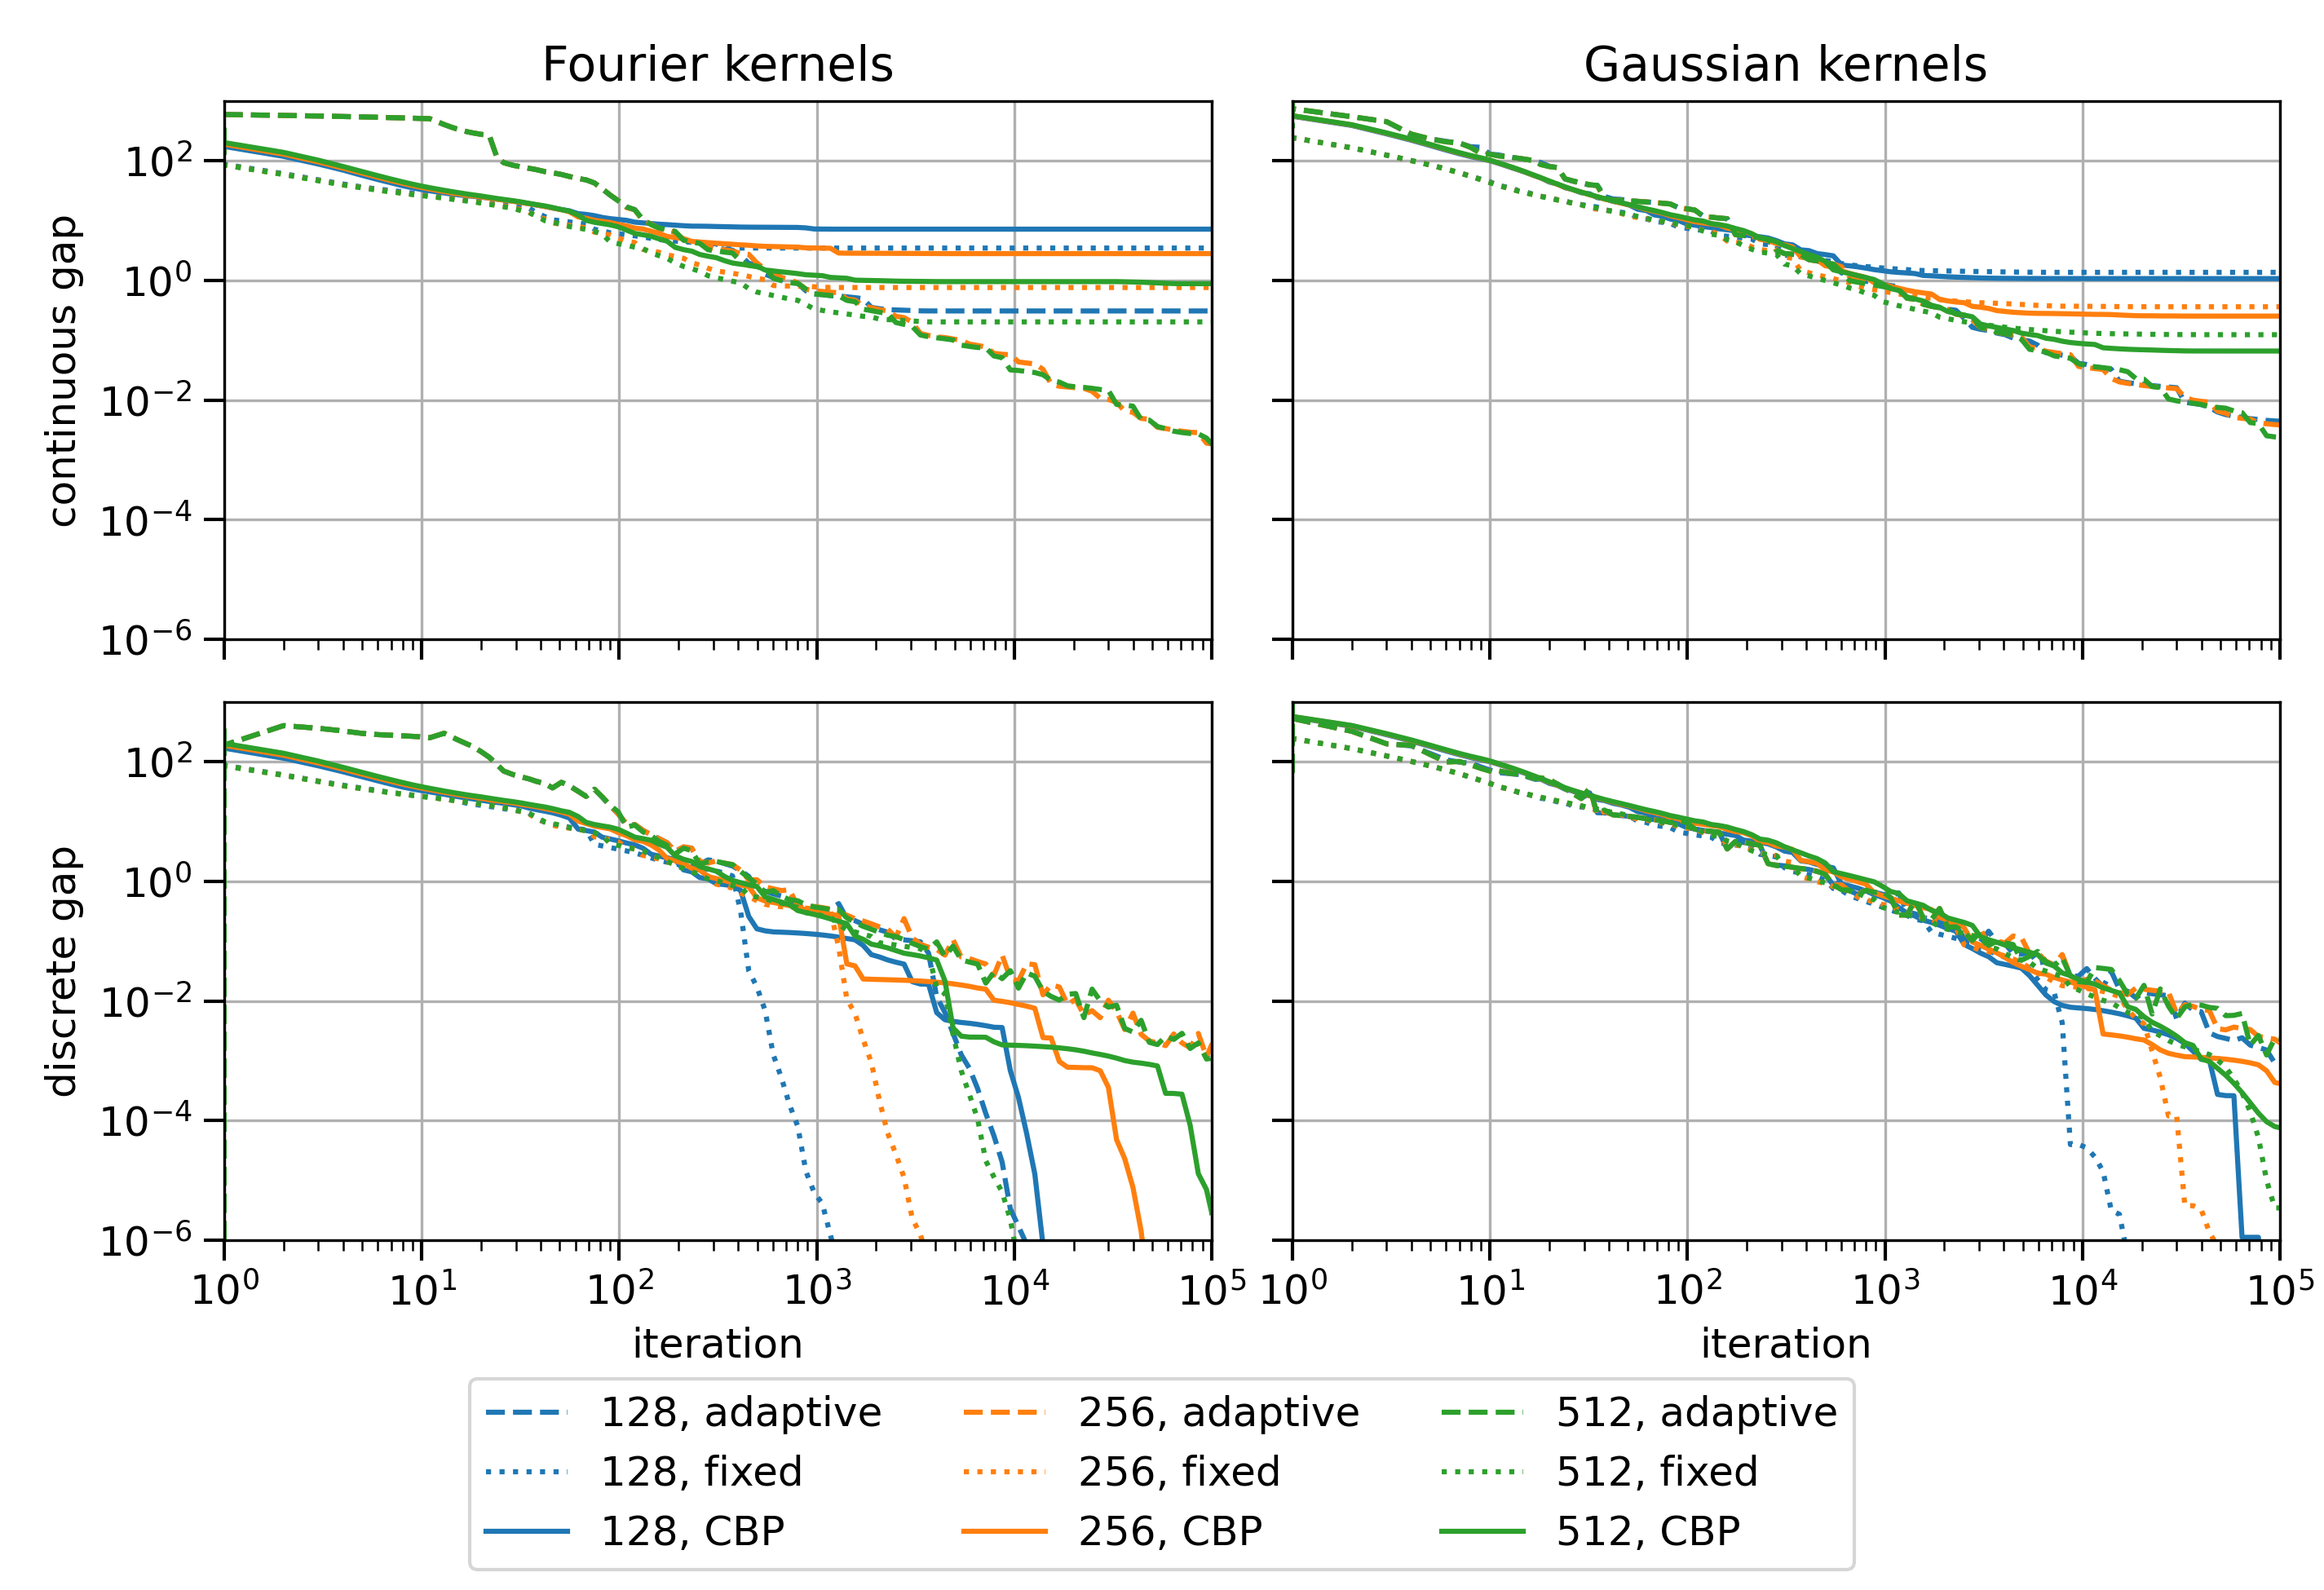
\includegraphics[width=.84\textwidth]{lasso_ndofs_convergence}
		\caption{Rates of continuous/discrete gap convergence for different Lasso algorithms with 128, 256, or 512 pixels. The `adaptive' method uses the proposed algorithm. Both `fixed' and `CBP' use standard FISTA with a uniform discretisation.}\label{fig: convergence with ndofs}
		
		\vspace*{\floatsep}
		
		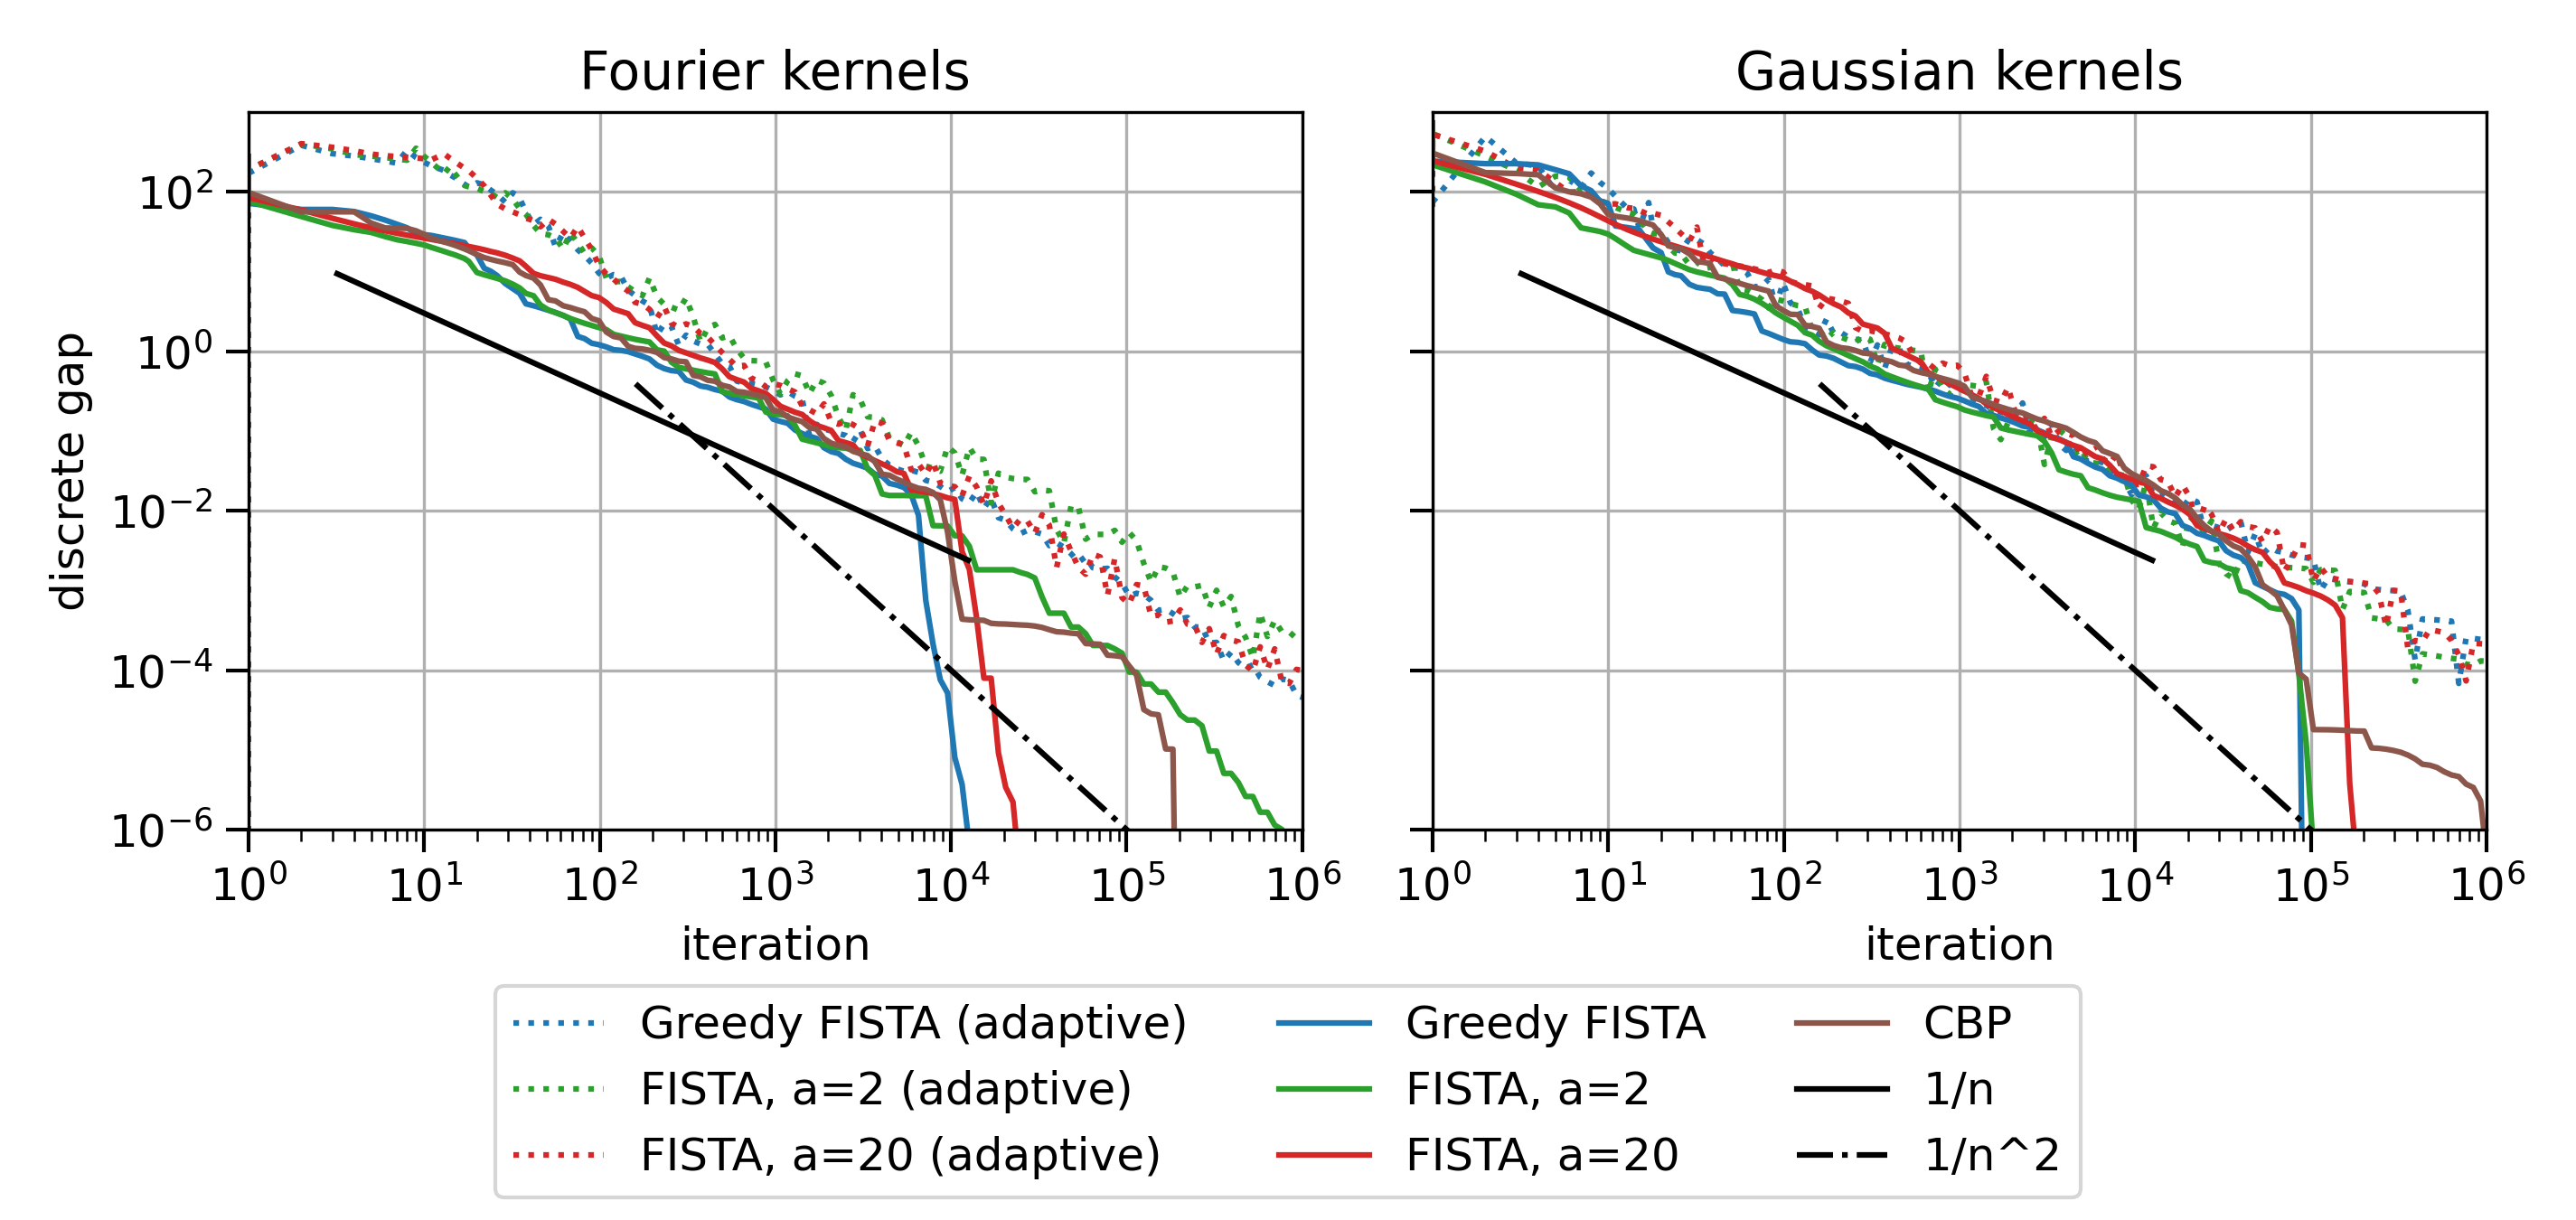
\includegraphics[width=.84\textwidth]{lasso_convergence_short}
		\caption{\edit{Discrete }{}Convergence plots for solving 1D problems with different algorithms. `Adaptive' methods use Algorithm~\ref{alg: refining FISTA} with fewer than 1024 pixels and the remaining methods use a uniform discretisation of 1024 pixels.}\label{fig: convergence with method}
	\end{figure}
	
	
	\paragraph{Comparison of FISTA variants}
	Figure~\ref{fig: convergence with method} compares many methods with either fixed or adaptive discretisations. Each adaptive scheme is allowed up to 1024 pixels and each uniform discretisation uses exactly 1024. The `Greedy FISTA' implementation was proposed by in \cite{Liang2018} and we include the adaptive variant despite a lack of convergence proof. The remaining FISTA algorithms use a FISTA time step of $t_n = \frac{n+a-1}{a}$ for the given value of $a$, as proposed in \cite{Chambolle2015}. In this example CBP used the greedy FISTA implementation which gave faster observed convergence. Figure~\ref{fig: convergence with method} compares the discrete gaps because it is the accurate metric for fixed discretisations, and for the adaptive discretisation it should also be an accurate predictor of the continuous gap. 
	
	The key observations are:
	\begin{itemize}
		\item Each algorithm displays very similar convergence properties. The main difference is that the reconstructions with fixed discretisations accelerate after $10^4$-$10^5$ iterations.
		\item During the initial `slow' phase, adaptive and fixed discretisations appear to achieve very similar (discrete) convergence rates. The coarse-to-fine adaptivity is not slower than fixed discretisations in this regime.
		\item Lemma~\ref{thm: practical refinement criteria} accurately predicts the $\frac1n$ rate of the adaptive methods, mirrored in the fixed discretisations. This suggests that high-resolution discretisations are also initially limited by this $\frac1n$ rate before entering the asymptotic regime.
		\item The fastest FISTA algorithm is consistently the greedy variant, although $a=20$ is very comparable.
	\end{itemize}
	
	\paragraph{Comparison of fixed and adaptive discretisation}
	Motivated by the findings in Figure~\ref{fig: convergence with method}, we now look more closely at the performance of the $a=20$ and the greedy FISTA schemes. We have analytical results for the former but the latter typically performs the best for non-adaptive optimisation and is never worse than $a=20$ in the adaptive setting. The question is whether it is faster/more efficient to use the proposed adaptive scheme or to use a classical scheme at sufficiently high uniform resolution. The fixed discretisations use 1024 pixels (i.e. constant pixel size of $2^{-10}$ in Figure~\ref{fig: comparison with iteration}) and the adaptive discretisation starts with two pixels with an upper limit of 1024. As expected, the fixed discretisation starts with a smaller continuous gap before plateauing to a sub-optimal gap around $\op{E}_0=0.1$.
	
	Figure~\ref{fig: comparison with iteration} shows convergence of pixel size and continuous gap with respect to number of iterations. Figure~\ref{fig: comparison with time} shows the more practical attributes of continuous gap and number of pixels against execution time. We see that the adaptive discretisation is consistently capable of computing lower energies with fewer pixels and in less time than the uniform discretisation. The convergence behaviour is very consistent with respect to number of iterations.
	
	Suppose that the numerical aim is to find a function $\varf0_n$ with $\op{E}_0(\varf0_n)\leq 0.1$, all methods would converge after $O(10^3)$ iterations, demonstrating some equivalence between the two FISTA algorithms. For $n\in[10^3,10^4]$, in both problems, the adaptive schemes coincide with the fixed schemes in both energy and minimum pixel size. On the other hand, we also see that the adaptive scheme achieves this energy in almost an order of magnitude less time and fewer pixels.
	
	\begin{figure}\centering
		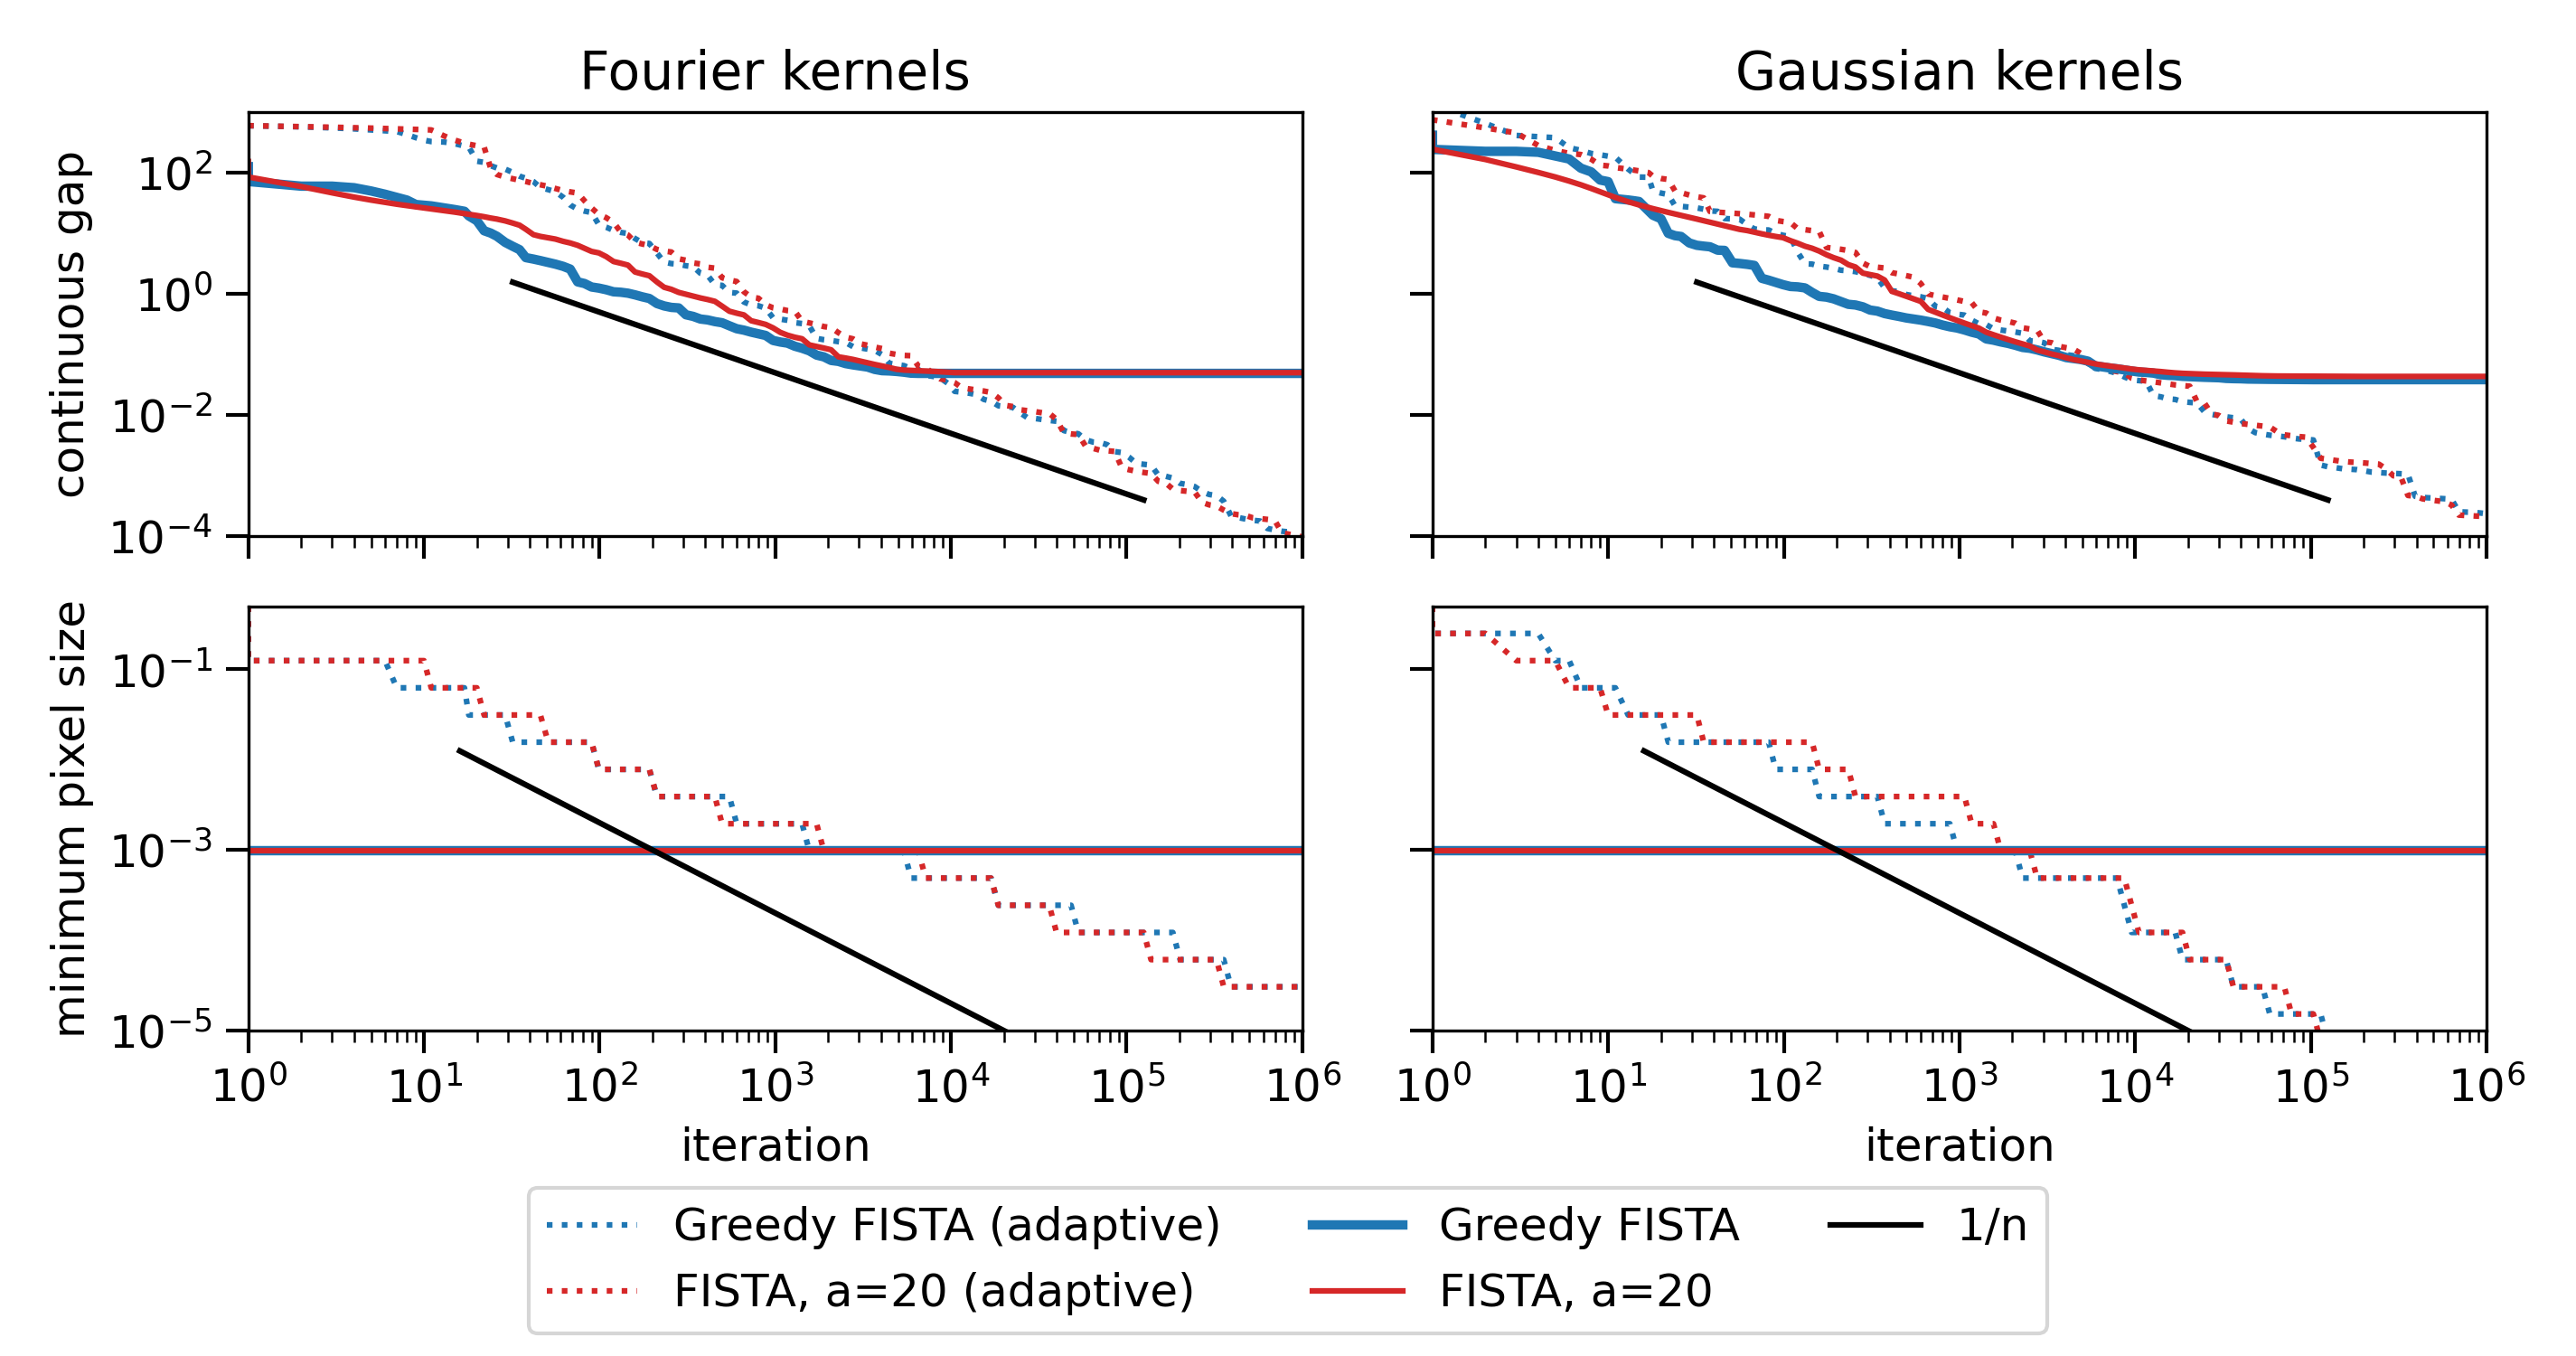
\includegraphics[width=.84\textwidth]{lasso_reduced_convergence}
		\caption{Continuous convergence of adaptive (coarse-to-fine pixel size) compared with uniform discretisation (constant pixel size) with respect to number of iterations. }\label{fig: comparison with iteration}
		
		\vspace*{\floatsep}
		
		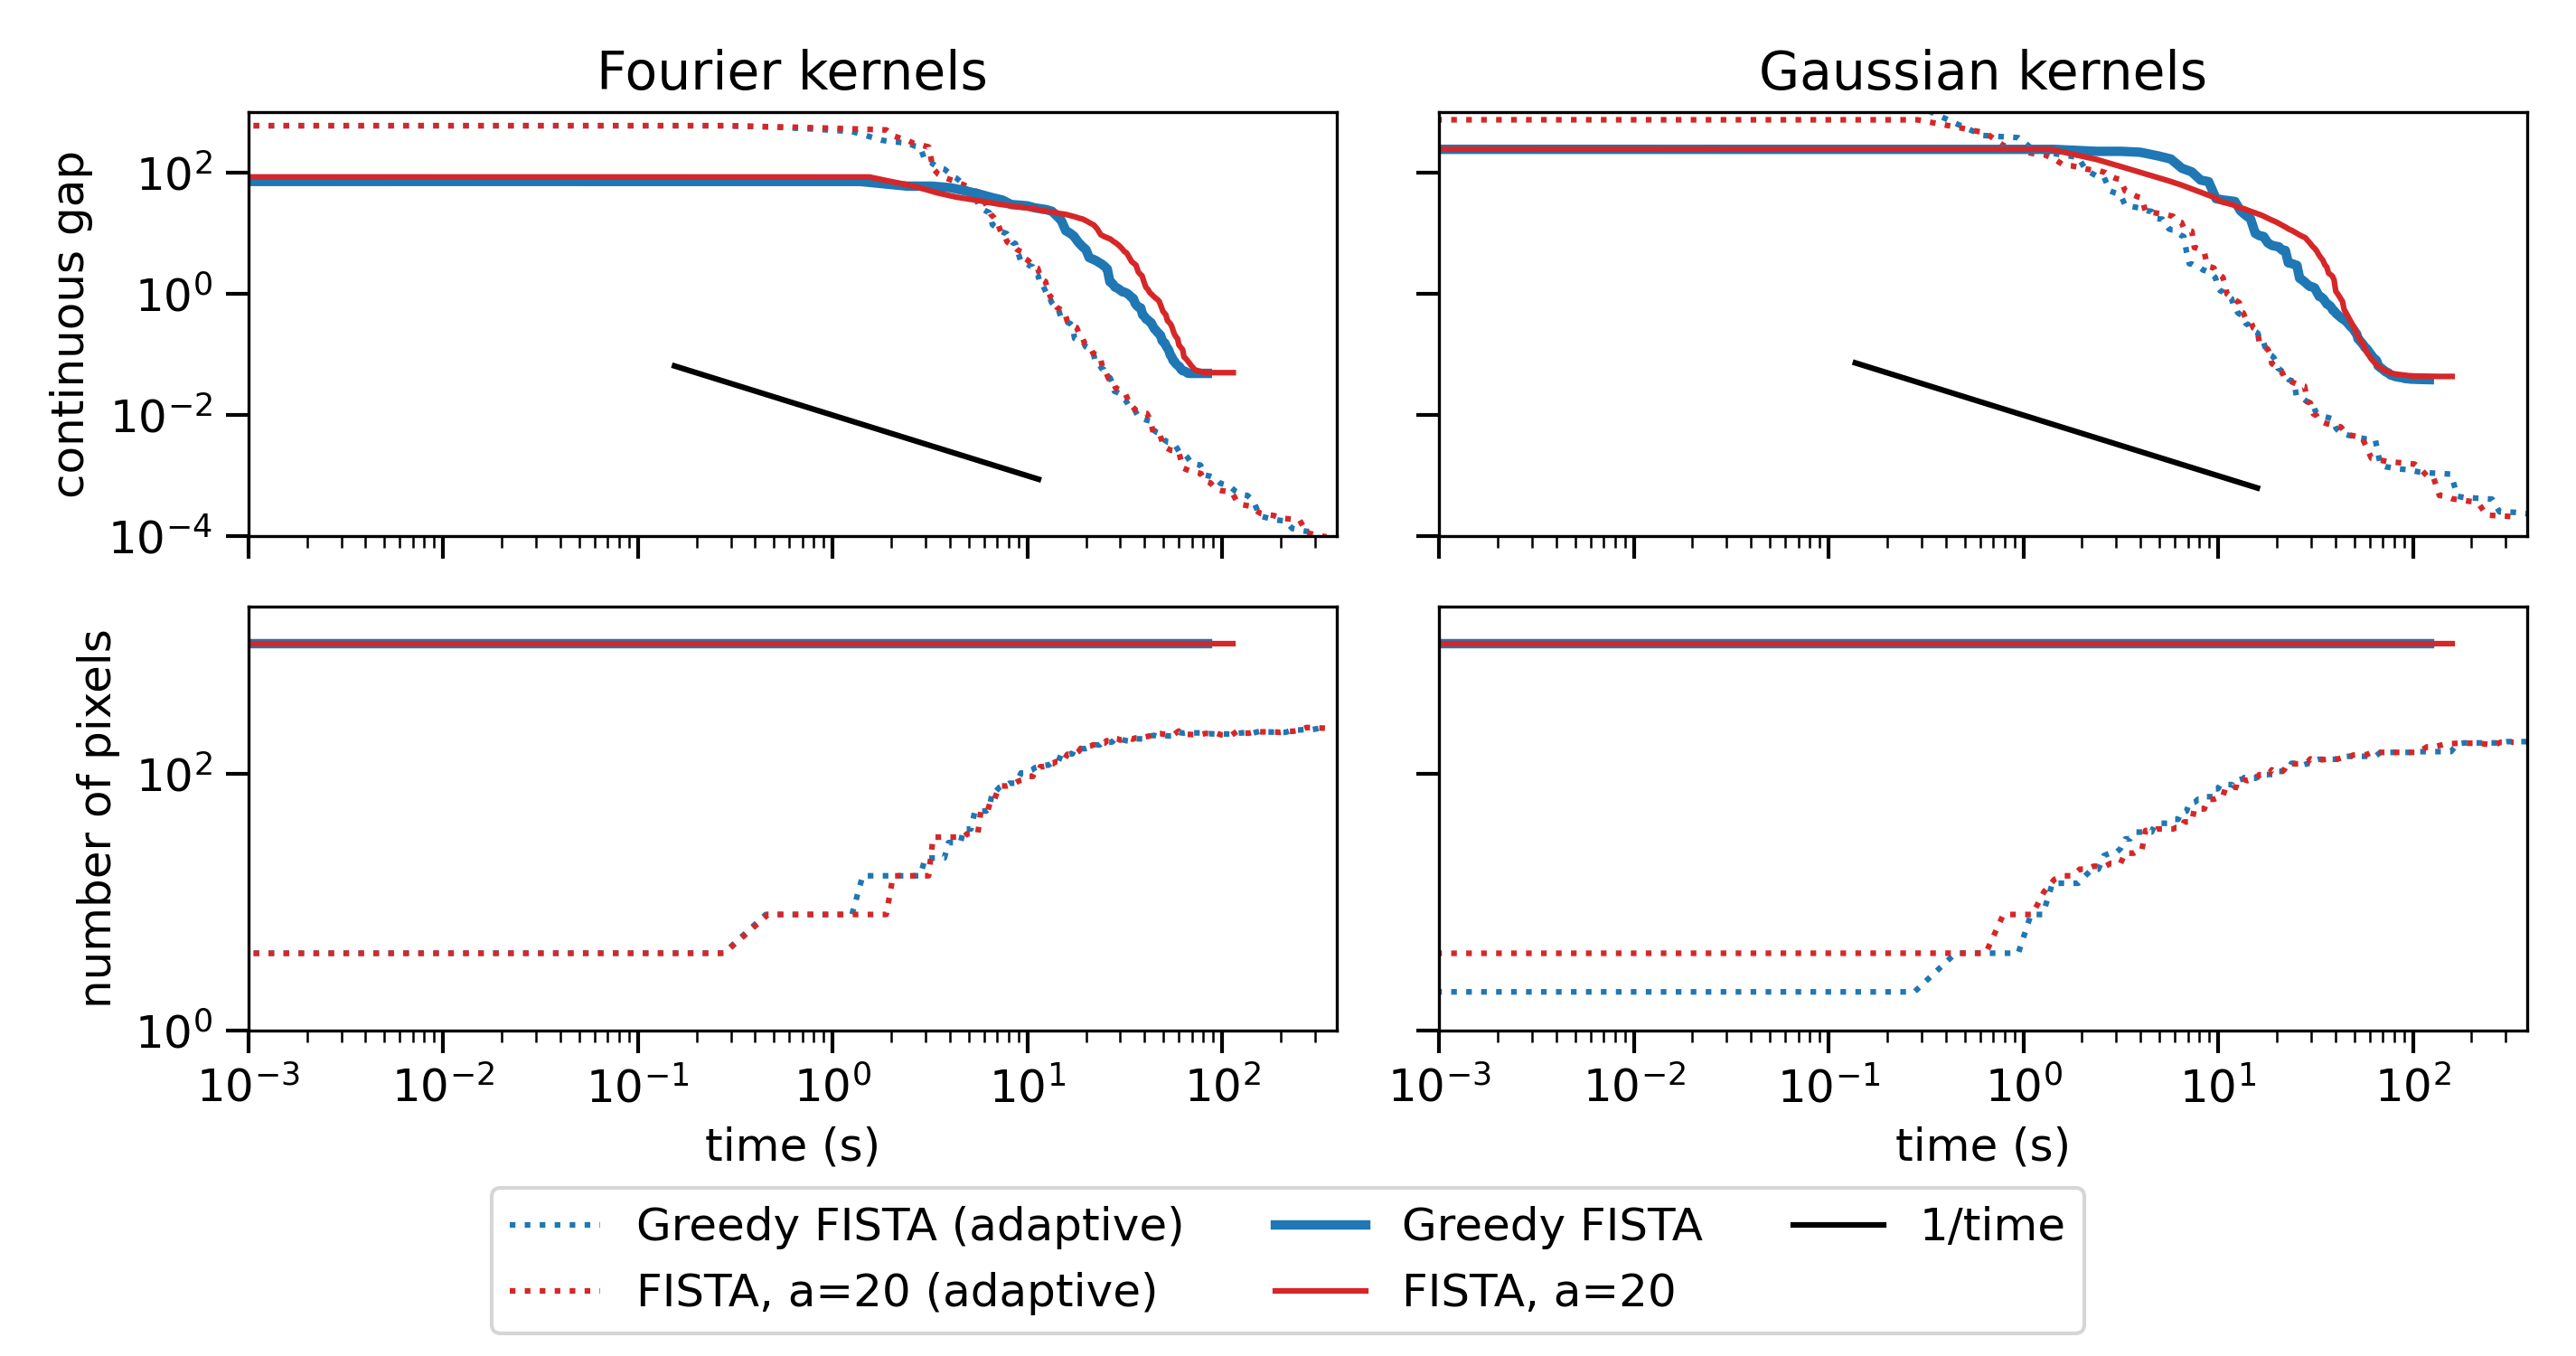
\includegraphics[width=.84\textwidth]{lasso_convergence_time}
		\caption{Continuous convergence of adaptive compared with uniform discretisation with respect to wall-clock time and total number of pixels (memory requirement).}\label{fig: comparison with time}
		
		\vspace*{\floatsep}
		
		\begin{center}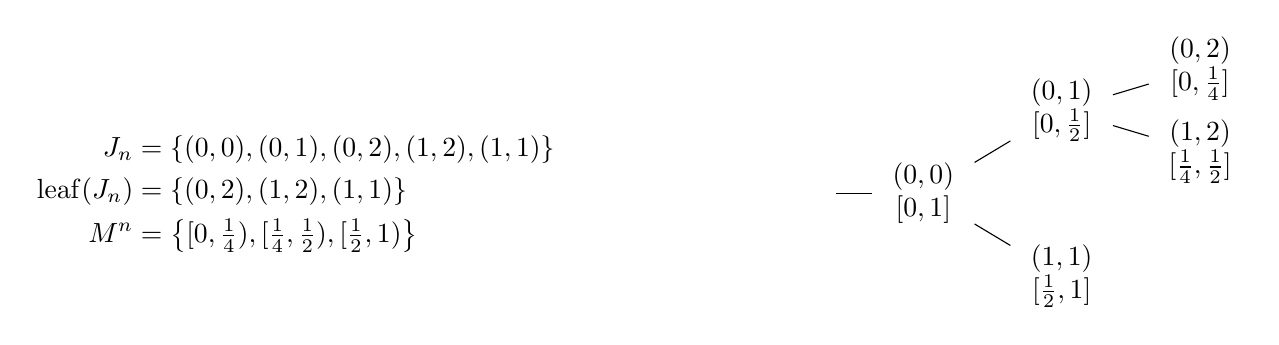
\begin{tikzpicture}[grow'=right]
				\tikzstyle{level 1}=[level distance=5em, sibling distance=0em];
				\tikzstyle{level 2}=[level distance=5em, sibling distance=6em];
				\tikzstyle{level 3}=[level distance=5em, sibling distance=3em];
				\tikzstyle{bag} = [text width=3em, text centered];
				
				\node[text width=7cm] at (-6cm,0) {
					$\begin{aligned}
						J_n &= \{(0,0), (0,1), (0,2), (1,2), (1,1)\}
						\\\op{leaf}(J_n) &= \{(0,2), (1,2), (1,1)\}
						\\\F M^n &= \left\{[0,\tfrac14),[\tfrac14,\tfrac12),[\tfrac12,1)\right\}
					\end{aligned}$ };
				
				\node[bag] at (0,0) {$ $}
				child {node[bag] {$(0,0)$ $[0,1]$}
					child {node[bag] {$(0,1)$ $[0,\frac12]$}
						child {node[bag] {$(0,2)$ $[0,\frac14]$}
						} child {node[bag] {$(1,2)$ $[\frac14,\frac12]$}
						}
					} child {node[bag] {$(1,1)$ $[\frac12,1]$}
				}};
		\end{tikzpicture}\end{center}
		\caption{Example tree representation of 1D wavelets. Left: nodes, leaves, and mesh of discretisation. Right: arrangement into a tree with index $(j,k)$ and corresponding support of wavelet $w_{j,k}$ underneath.}\label{fig: wavelet tree}
	\end{figure}
	
	\subsection{2D wavelet Lasso}\label{sec: wavelet examples}
	In this example we consider $\A$ to be a 2D Radon transform. In particular, the rows of $\A$ correspond to integrals over the sets $\F{X}^I_i$ where 
	\begin{equation}
		\F{X}_i^I = \left\{\vvarx0\in[-\tfrac12,\tfrac12]^2\st \ip{\vvarx0}{\begin{pmatrix}\cos\theta_I\\\sin\theta_I\end{pmatrix}}\in \left[-\tfrac12+\tfrac{i-1}{50},-\tfrac12+\tfrac{i}{50}\right)\right\}, \quad \theta_I=\frac{180^\circ}{51}I \quad \text{ for } i,I=1,2,\ldots,50.
	\end{equation}
	This is not exactly in the form analysed by Theorem~\ref{thm: norm bound examples}, however only the sets $\{\F{X}^I_i\st i\in[50]\}$ for each $I$ are disjoint, therefore we apply Theorem~\ref{thm: norm bound examples} block-wise to estimate
	\begin{equation}
		\norm{\A}_{L^2\to\ell^2} \leq \sqrt{\sum_{I\in[50]}\max_{i\in[50]} |\F{X}^I_i|} = \sqrt{\sum_{I\in[50]}\max_{i\in[50]} \int_{\F{X}^I_i}1d\vvarx0}= \sqrt{\sum_{I\in[50]}\max_{i\in[50]}\ (\A\1)_{i,I}}\;.
	\end{equation}
	$\A$ is not smooth, therefore we can't bound $|\A^*|_{C^k}$ for $k>0$, and so we must look to minimise over $\ell^1$ rather than $L^1$. The natural choice is to promote sparsity in a wavelet basis which can be rearranged into the Lasso form:
	\begin{equation}
		\min_{\varf0\in \spcf0} \tfrac12\norm{\A\varf0-\data}_{\ell^2}^2 + \mu \norm{\tens{W}^{-1}\varf0}_{\ell^1} = \min_{\hat{\varf0}\in\ell^1(\R)} \tfrac12\norm{\A\tens{W}\hat{\varf0}-\data}_{\ell^2}^2 + \mu \norm{\hat{\varf0}}_{\ell^1}.
	\end{equation}
	The minimisers are related by $\varf0^* = \tens{W}\hat{\varf0}^*$ and, for wavelet bases, $\tens{W}$ is orthonormal so $\norm{\A\tens{W}}_{\ell^2\to\ell^2} = \norm{\A}_{L^2\to\ell^2}$. From Section~\ref{sec: Lasso gap and gradient} we know that to track convergence and perform adaptive refinement, it is sufficient to accurately bound $|[\tens{W}^\top \A^*\vvard0_n]_j|$ for all $j\notin J_n$. If $\tens{W}$ is a wavelet transformation then its columns, $w_j\in L^2$, are simply the wavelets themselves and we can use the bound 
	\begin{equation}
		|\IP{w_j}{\A^*\vvard0_n}| = \left|\IP{w_j}{\1_{\supp(w_j)}\A^*\vvard0_n}\right| \leq \norm{\1_{\supp(w_j)} \A^*\vvard0_n}_{L^2}\leq \norm{\1_{\F{X}} \A^*\vvard0_n}_{L^2}
	\end{equation}
	for all $\F{X}\supset \supp(w_j)$.
	In the case of the Radon transform, we can compute the left-hand side explicitly for the finitely many $j\in J_n$ but we wish to use the right-hand side in a structured way to avoid computing the infinitely many $j\notin J_n$. To do this, we will take a geometrical perspective on the construction of wavelets to view them in a tree format. 
	
	\paragraph{Tree structure of wavelets}
	Finite elements are constructed with a mesh which provided a useful tool for adaptive refinement in Section~\ref{sec: bound continuous}. For wavelets, we will associate a tree with every discretisation and the leaves of the tree correspond to a mesh. This perspective comes from the multi-resolution interpretation of wavelets. An example is seen in Figure~\ref{fig: wavelet tree} for 1D Haar wavelets, $w_{j,k}(\varx0) = \sqrt{2}^k\vard1(2^{k}\varx0-j)$ where $\vard1 = \1_{[0,1)} - \1_{[-1,0)}$. 
	
	In higher dimensions, the only two things which change are the number of children ($2^d$ for non-leaves) and at each node you store the coefficients of $2^d-1$ wavelets. The support on each node is still a disjoint partition of unity consisting of regular cubes of side length $2^{-k}$ at level $k$. The only change in our own implementation is to translate the support to $[-\tfrac12,\tfrac12]^2$. We briefly remark that the tree structuring of wavelets is not novel and appears more frequently in the Bayesian inverse problems literature \cite{Castillo2019,Kekkonen2021}.
	
	\paragraph{Continuous gradient estimate}
	In Section~\ref{sec: 1D Lasso examples} we used the continuous gap as a measure for convergence, for wavelets we will use the continuous \edit{gradient}{subdifferential}. With the tree structure we can easily adapt the results of Section~\ref{sec: Lasso gap and gradient} to estimate \edit{gradients}{subdifferentials} (or function gaps). In particular,
	\begin{align}
		\Norm{\partial \op{E}(\varf0_n)}_* &=\max\left(\Norm{\partial_n\op{E}(\varf0_n)}_*, \max_{j\notin J_n} |\IP{w_j}{\A^*\vvard0_n}| -\mu \right) \\&\leq\max\left(\Norm{\partial_n\op{E}(\varf0_n)}_*, \max_{j\in \op{leaf}(J_n)} \norm{\1_{\supp(w_j)}\A^*\vvard0_n}_{L^2} -\mu \right).\label{eq: wavelet error metric}
	\end{align}
	
	\paragraph{Numerical results}
	We consider two phantoms where the ground-truth is either a binary disc or the Shepp-Logan phantom. No noise is added to the Shepp-Logan data but \SI{5}{\percent} Gaussian white noise is added to the disc data. This is visualised in Figure~\ref{fig: haar data}. All optimisations shown will be spatially adaptive using Haar wavelets and initialised with $\spcf0^0= \{\varx0\mapsto c\st c\in\F R\}$. The gradient metric shown throughout is the $\ell^2$ norm. Motivated by \eqref{eq: wavelet error metric}, the spatial adaptivity is chosen to refine nodes $j\in\op{leaf}(J_n)$ to ensure that 
	$$ \norm{\1_{\supp(w_j)}\A^*\vvard0_n}_{L^2} -\mu  \leq 10\Norm{\partial_n\op{E}(\varf0_n)}_*$$
	for all $j$ and $n$ (i.e. so that the continuous gradient is less than 10 times the discrete gradient).
	
	The first numerical results shown in Figure~\ref{fig: haar convergence} compare the same adaptive algorithms as shown in Figure~\ref{fig: convergence with method}. In these examples we see that the greedy FISTA and the $a=20$ algorithms achieve almost linear convergence while $a=2$ is significantly slower.
	
	\begin{figure}\centering
		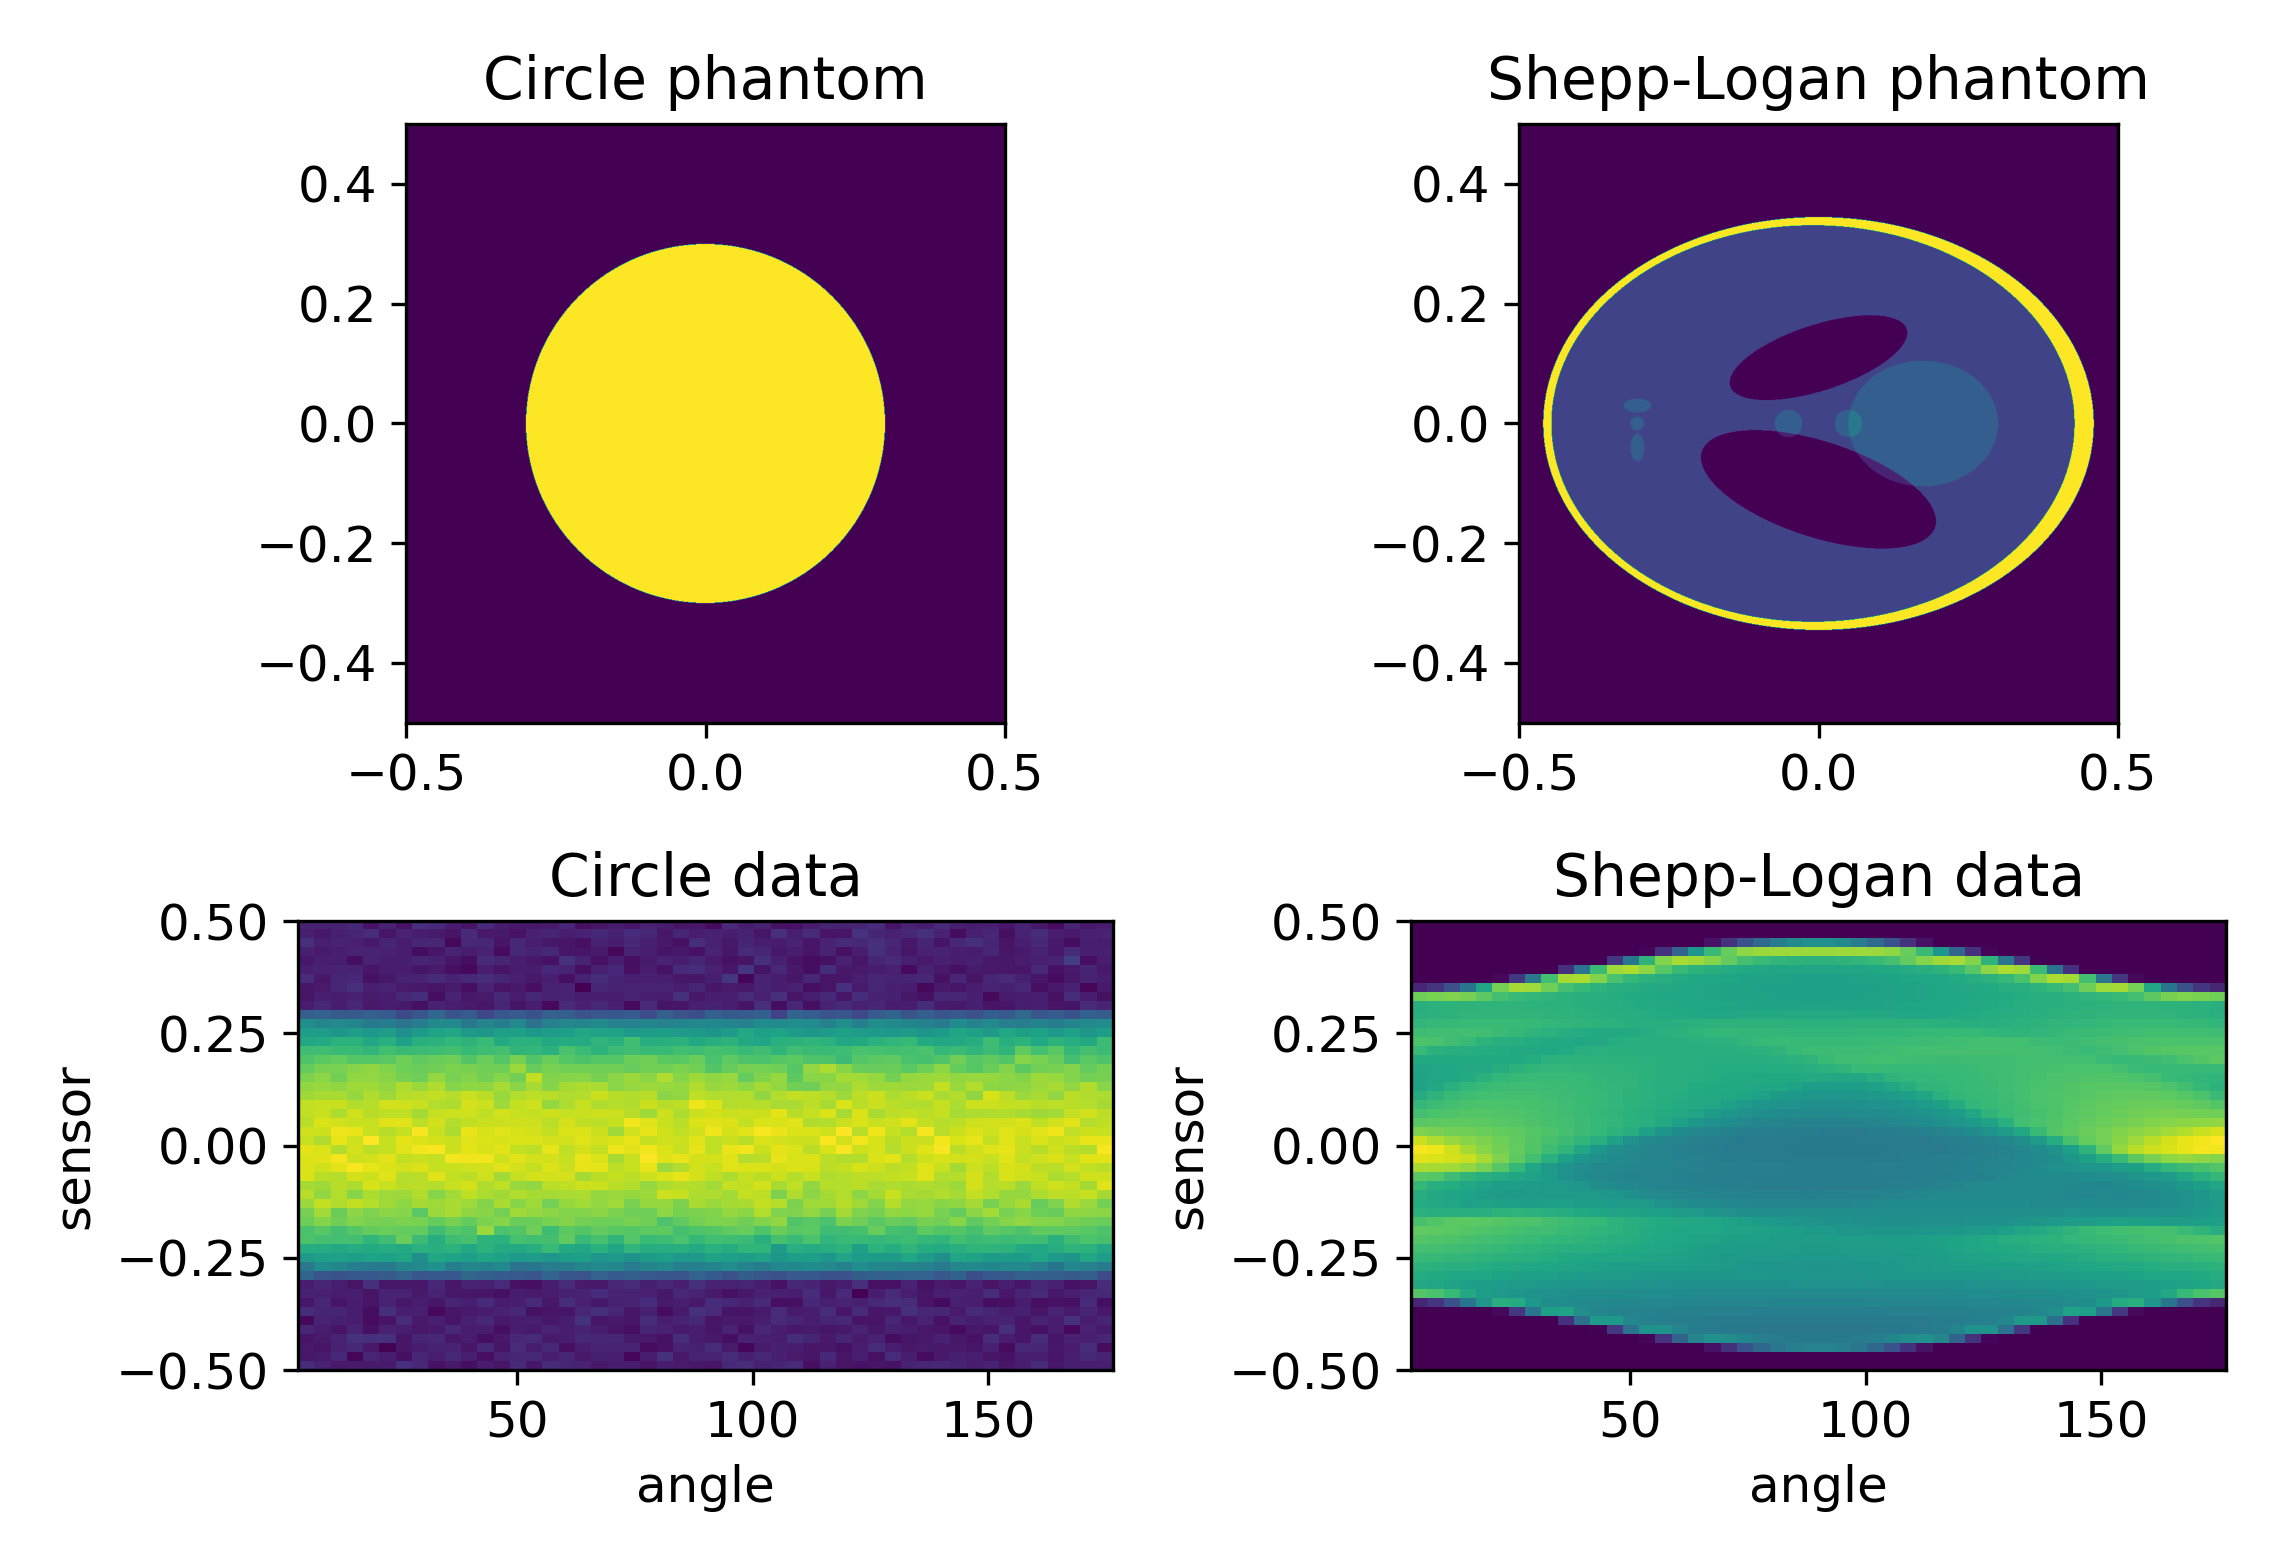
\includegraphics[width=.85\textwidth]{haar_data}
		\caption{Phantoms and data used for wavelet-sparse tomography optimisation. The Shepp-Logan data is exact but the data for the disc-phantom has \SI{5}{\percent}\ Gaussian white noise. Without noise the data would be uniform with respect to the angle.}\label{fig: haar data}
		
		\vspace*{\floatsep}
		
		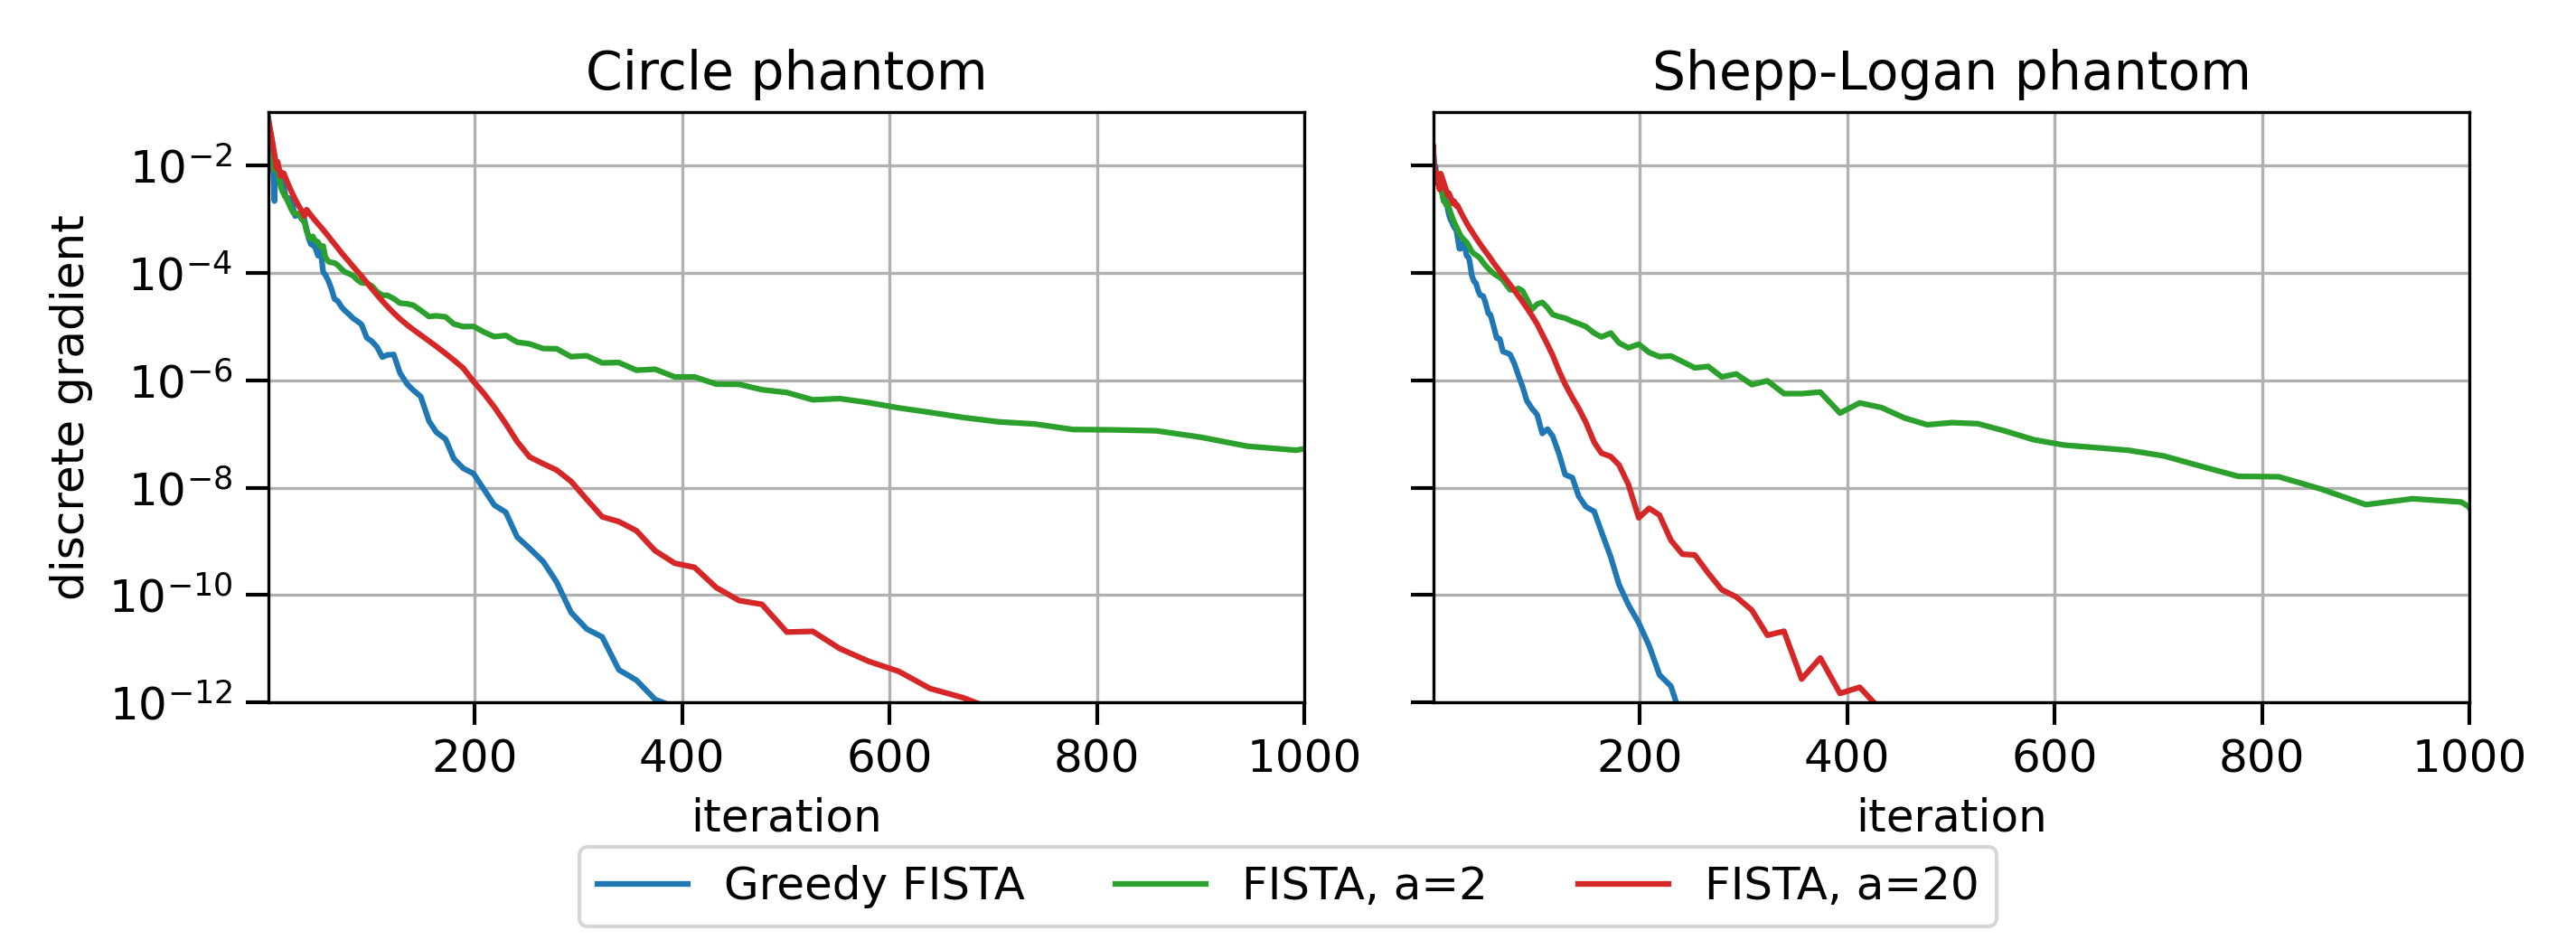
\includegraphics[width=.85\textwidth]{haar_convergence_short}
		\caption{\edit{Discrete }{}Convergence of different implementations of Algorithm~\ref{alg: refining FISTA} with an unlimited number of pixels.}\label{fig: haar convergence}
		
		\vspace*{\floatsep}
		
		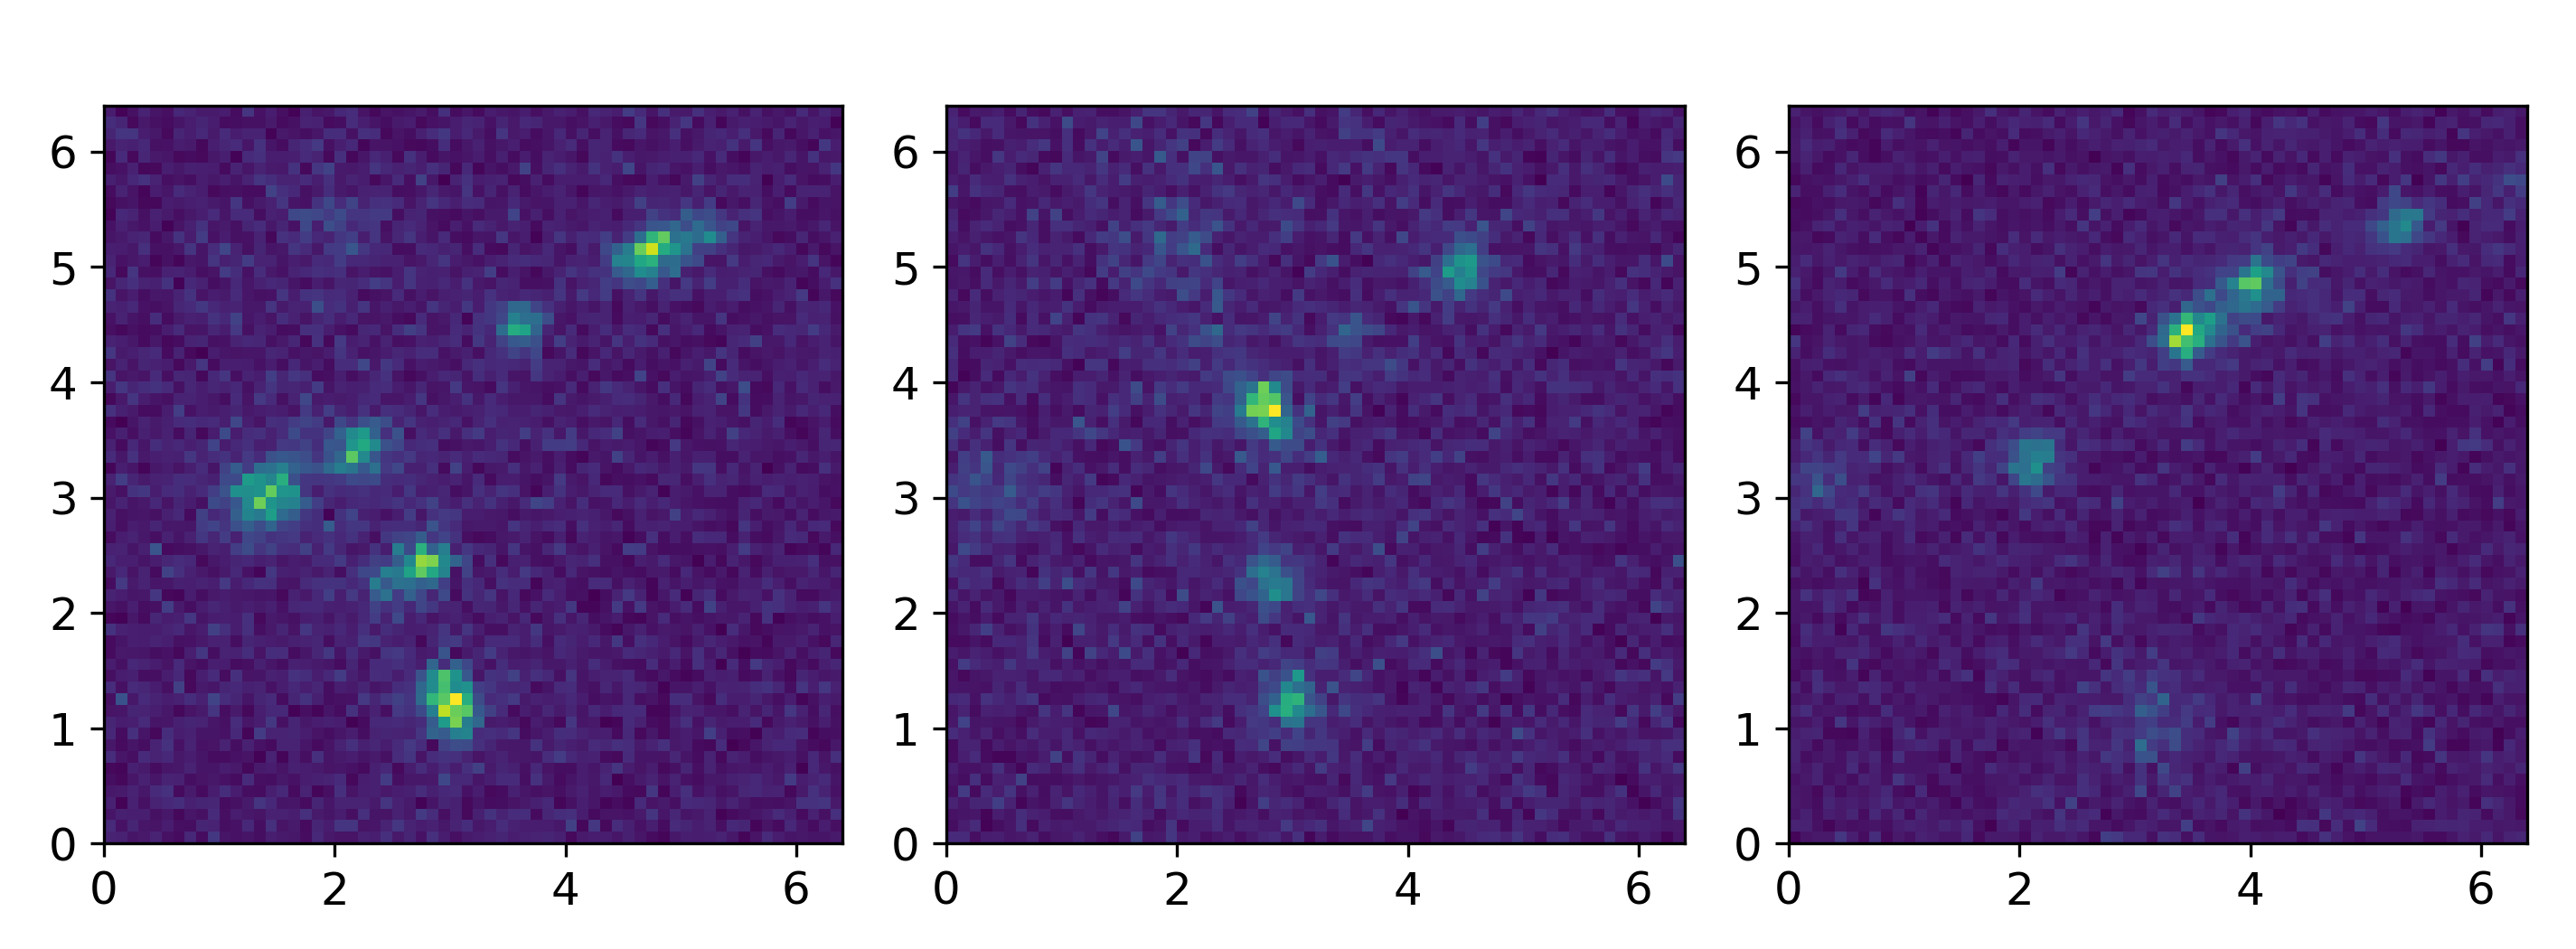
\includegraphics[width=.85\textwidth]{STORM_data}
		\caption{Example images from STORM dataset.}\label{fig: STORM data}
	\end{figure}
	
	\subsection{2D continuous Lasso}
	Our final application is a super-resolution/de-blurring inverse problem from biological microscopy. In mathematical terms, the observed data is a large number of sparse images which are corrupted by blurring and a large amount of noise, examples are seen in Figure~\ref{fig: STORM data}. The task is to compute the centres of the spikes of signal in each image and then re-combine into a single super-resolved image, as in Figure~\ref{fig: STORM results}. This technique is referred to as \emph{Single Molecule Localisation Microscopy} (SMLM), of which we consider the specific example of \emph{Stochastic Optical Reconstruction Microscopy} (STORM). Readers are directed to the references \cite{Sage2015,Sage2019,Schermelleh2019} for further details. The Lasso formulation has previously been shown to be effective in the context of STORM \cite{Huang2017,Denoyelle2019}.
	
	Here we use a simulated dataset provided as part of the 2016 SMLM challenge\footnote{\url{http://bigwww.epfl.ch/smlm/challenge2016/datasets/MT4.N2.HD/Data/data.html}} for benchmarking software in this application. The corresponding Lasso formulation is 
	\begin{equation}
		(\A\varf0)_{i} = (2\pi\sigma^2)^{-1}\int_{[0,6.4]^2} \exp\left(-\frac{1}{2\sigma^2}\left|\vvarx0- \Delta\begin{pmatrix}i_1+\tfrac12 & i_2+\tfrac12\end{pmatrix}^\top \right|^2\right)\varf0(\vvarx0)\,d\vvarx0, \qquad \sigma=0.2,\ \Delta=0.1
	\end{equation}
	for $i_1,i_2 = 1,2,\ldots,64$ and $\spcf0=\C M([0,6.4]^2)$ with lengths in $\SI{}{\micro\meter}$. 3020 frames are provided, examples of which are shown in Figure~\ref{fig: STORM data}. To process this dataset, image intensities were normalised to $[0,1]$ then a constant was subtracted to approximate 0-mean noise. The greedy FISTA algorithm was used for optimisation with $\mu=0.15$, $10^3$ iterations, and a maximum of $10^5$ pixels per image. 
	
	Finally, all the reconstructions were summed and the result shown in Figure~\ref{fig: STORM results}. The adaptive scheme used fewer than $10^4$ pixels per frame, a fixed discretisation with equivalent resolution of \SI{1.3}{\nano\meter} would have required more than $3\cdot10^6$ per frame. Lasso is compared with ThunderSTORM \cite{Ovesny2014}, a popular ImageJ plugin \cite{Schindelin2012} which finds the location of signal using Fourier filtering. The performance of ThunderSTORM was rated very highly in the initial SMLM challenge \cite{Sage2015}. Both methods compared here demonstrate the key structures of the reconstruction, however, both are sensitive to tuning parameters. In this examples, Lasso has possibly recovered too little signal and ThunderSTORM contains spurious signal. 
	
	Figure~\ref{fig: STORM convergence} shows slightly faster convergence than $n^{-2/3}$ predicted by \eqref{eq: Lasso resolution rate} in dimension $d=2$. In this example we also implement the suggestion of Section~\ref{sec: support detection} to remove pixels outside of the support of $\varf0^*$. From \eqref{eq: support equation}, any pixel $\domain_i^n$ satisfying 
	\begin{equation}
		\vars2_0 \norm{ \tens{\Pi}_n\A^*\vvard0_n }_{L^\infty(\domain_i^n)} \leq (1-\op{threshold}_n)\mu
	\end{equation}
	guarantees that $\domain_i^n\cap\op{supp}(\varf0^*) = \emptyset$. This threshold is plotted in the first panel of Figure~\ref{fig: STORM convergence}. Once the value becomes less than 1, we can start reducing the number of pixels instead of continual refinement, as seen in the right-hand panel after around 30 iterations.
	
	\begin{figure}\centering
		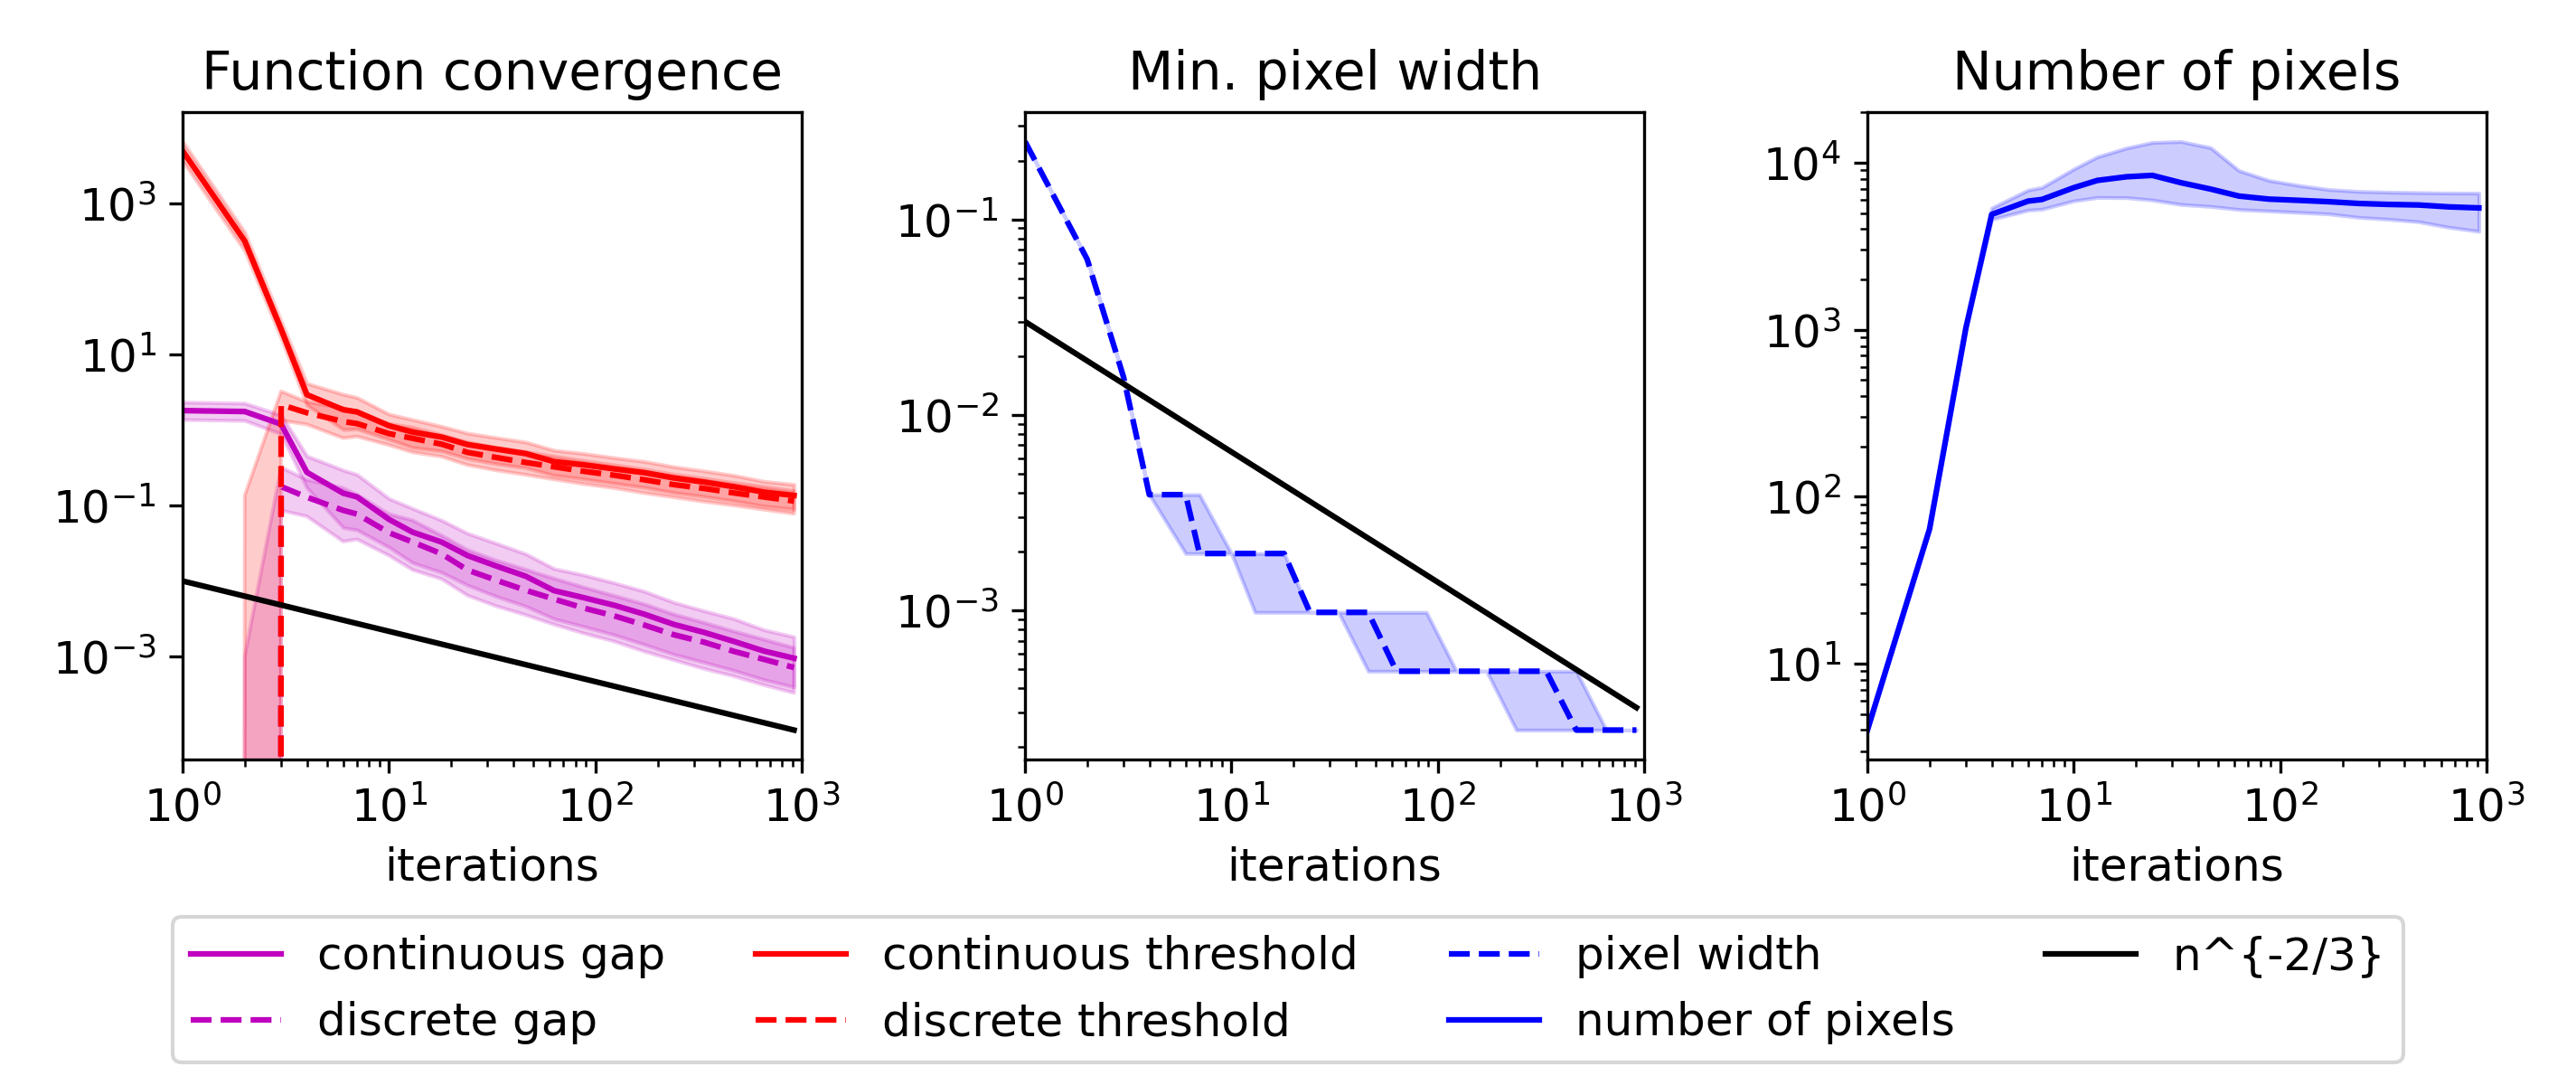
\includegraphics[width=.82\textwidth]{lasso2_convergence}
		\caption{Convergence of adaptive FISTA for STORM dataset. Lines indicate the median value over 3020 STORM frames. Shaded regions indicate the \SIrange{25}{75}{\percent} inter-quartile range. Pixel width is scaled $[0,1]$ rather than $[0,\SI{6.4}{\micro\meter}]$.}\label{fig: STORM convergence}
		
		\vspace*{\floatsep}
		
		\includegraphics[width=.73\textwidth]{STORM_recon}
		\caption{Processed results of the STORM dataset. Top left: Lasso optimisation with Algorithm~\ref{alg: refining FISTA}. Top right: Comparison with ThunderSTORM plugin. Bottom: Average data, no super-resolution or de-blurring.}\label{fig: STORM results}
	\end{figure}
	
	\section{Conclusions and outlook}
	In this work we have proposed a new adaptive variant of FISTA and provided convergence analysis. This algorithm allows FISTA to be applied outside of the classical Hilbert space setting, still with a guaranteed rate of convergence. We have presented several numerical examples where convergence with the refining discretisation is at least as fast as a uniform discretisation, although more efficient with regards to both memory and computation time. 
	
	In 1D we see good agreement with the theoretical rate. This rate also seems to be a good predictor for all variants of FISTA tested, although this is yet to be proven. Surprisingly, even the classical methods with a fixed discretisation initially seem limited to the slower adaptive rate for small $n$.
	
	The results in 2D are similar, all tested FISTA methods converge at least at the guaranteed rate. The wavelet example was most impressive, achieving nearly linear convergence in energy. This is similar to the behaviour for classical FISTA although it is also yet to be formally proven.
	
	An interesting observation over all of the adaptive Lasso examples is that the standard oscillatory behaviour of FISTA has not occurred. With the monotone gaps plotted, oscillatory convergence should correspond to a piecewise constant descending gap. Either this behaviour only emerges for larger $n$, or the adaptivity provides a dampening effect for this oscillation.
	
	Moving forward, it would be interesting to see how far the analysis extends to other optimisation algorithms. Other variants of FISTA, such as the `greedy' implementation used here or the traditional Forward-Backward algorithm, should also be receptive to the analysis performed here. Furthermore, it would also interesting to attempt to replicate this refinement argument to extend the primal-dual algorithm \cite{Chambolle2011} or the Douglas-Rachford algorithm \cite{Douglas1956}.
	
	\begin{acknowledgements}
		R.T. acknowledges funding from EPSRC grant EP/L016516/1 for the Cambridge Centre for Analysis, and the ANR CIPRESSI project grant ANR-19-CE48-0017-01 of the French Agence Nationale de la Recherche. Most of this work was done while A.C. was still in CMAP, CNRS and Ecole Polytechnique, Institut Polytechnique de Paris, Palaiseau, France.
	\end{acknowledgements}
	\begingroup
	\bibliography{references}
	\endgroup
	\appendix
	\section{Proofs for FISTA convergence}\label{app: FISTA convergence}
	This section contains all of the statements and proofs of the results contained in Section~\ref{sec: FISTA convergence}. \edit{}{Recall that the subsets $\spcf0^n\subset\F H$ satisfy \eqref{eq: refining subspace definition}.}
	
	\subsection{Proofs for Step 3}
	
	\begin{theorem}[Lemma~\ref{thm: one step FISTA}]\label{app:thm: one step FISTA}
		\Paste{thm: one step FISTA}
		\begin{equation}
			t_{n}^2(\op{E}(\varf0_{n}) - \op{E}(\varf2_n)) - (t_{n}^2-t_{n})(\op{E}(\varf0_{n-1})-\op{E}(\varf2_n)) \leq \tfrac1{2}\left[\norm{\varf1_{n-1}}^2-\norm{\varf1_{n}}^2\right] + \IP{\varf1_{n}-\varf1_{n-1}}{\varf2_n}.
			\label{app:eq: one-step FISTA}
		\end{equation}
	\end{theorem}
	\begin{proof}
		Modifying \cite[\edit{Theorem 2}{Thm 3.2}]{Chambolle2015}, for $n\geq1$ we apply Lemma~\ref{thm: descent lemma} with $\bar{\varf0} = \bar{\varf0}_{n-1}$ and $\varf2 = (1-\frac{1}{t_{n}})\varf0_{n-1} + \frac{1}{t_{n}}\varf2_n$. \edit{}{By \eqref{eq: refining subspace definition}, $\varf0_{n-1}\in\spcf0^n$ is convex so $\varf2\in \spcf0^n$. }This gives
		\begin{equation}
			\op{E}(\varf0_{n}) + \tfrac12\norm{\tfrac{1}{t_{n}}\varf1_{n}-\tfrac{1}{t_{n}}\varf2_n}^2 \leq \op{E}\left((1-\tfrac{1}{t_{n}})\varf0_{n-1}+\tfrac{1}{t_{n}}\varf2_n\right) + \tfrac12\norm{\tfrac{1}{t_{n}}\varf1_{n-1}-\tfrac{1}{t_{n}}\varf2_n}^2.
		\end{equation}
		By the convexity of $\op{E}$, this reduces to
		\begin{equation}
			\op{E}(\varf0_{n}) - \op{E}(\varf2_n) - (1-\tfrac{1}{t_{n}})[\op{E}(\varf0_{n-1})-\op{E}(\varf2_n)] \leq \tfrac1{2t_{n}^2}\norm{\varf1_{n-1}-\varf2_n}^2 - \tfrac1{2t_{n}^2}\norm{\varf1_{n}-\varf2_n}^2 = \tfrac1{2t_{n}^2}\left[\norm{\varf1_{n-1}}^2-\norm{\varf1_{n}}^2\right] + \tfrac1{t_{n}^2}\IP{\varf1_{n}-\varf1_{n-1}}{\varf2_n}.
		\end{equation}
		\edit{}{Multiplying through by $t_n^2$ gives the desired inequality.}
		\qed\end{proof}
	
	
	
	\begin{theorem}[Theorem~\ref{thm: mini FISTA convergence}]\label{app:thm: mini FISTA convergence}
		\Paste{thm: mini FISTA convergence}
		\begin{equation}\label{app:eq: FISTA inequality}
			\Paste{thm:eq: mini FISTA convergence}
		\end{equation}
	\end{theorem}
	\begin{proof}
		Theorem~\ref{app:thm: mini FISTA convergence} is just a summation of \eqref{app:eq: one-step FISTA} over all $n=1,\ldots,N$. To see this: first add and subtract $\edit{\op{E}(\varf0^*)}{\Emin}$ to each term on the left-hand side to convert $\op{E}$ to $\op{E}_0$, then move $\op{E}_0(\varf2_n)$ to the right-hand side. Now \eqref{app:eq: one-step FISTA} becomes
		\begin{equation}
			t_n^2\op{E}_0(\varf0_n) - (t_n^2-t_n)\op{E}_0(\varf0_{n-1}) \leq t_n\op{E}_0(\varf2_n) + \tfrac1{2}\left[\norm{\varf1_{n-1}}^2-\norm{\varf1_n}^2\right] + \IP{\varf1_n-\varf1_{n-1}}{\varf2_n}. 
		\end{equation}
		Summing this inequality from $n=1$ to $n=N$ gives
		\begin{equation}
			t_N^2\op{E}_0(\varf0_N) + \sum_{n=1}^{N-1}(\underbrace{t_n^2-t_{n+1}^2+t_{n+1}}_{=\rho_n})\op{E}_0(\varf0_n) \leq \frac{\norm{\varf1_0}^2-\norm{\varf1_N}^2}{2} + \sum_{n=1}^N t_n\op{E}_0(\varf2_n)+\IP{\varf1_n-\varf1_{n-1}}{\varf2_n}.
		\end{equation}
		This is almost in the desired form, however, we would like to flip the roles of $\varf1_n$/$\varf2_n$ in the final inner product term. Re-writing the right-hand side gives
		\begin{equation}
			\sum_{n=1}^N\IP{\varf1_n-\varf1_{n-1}}{\varf2_n} = \IP{\varf1_N}{\varf2_N} - \IP{\varf1_0}{\varf2_0}+ \sum_{n=1}^N\IP{\varf1_{n-1}}{\varf2_{n-1}-\varf2_n}.
		\end{equation}
		Noting that $\varf1_0=\varf0_0$, the previous two equations combine to prove the statement of Theorem~\ref{app:thm: mini FISTA convergence}.
		\qed\end{proof}
	
	The following lemma is used to produce a sharper estimate on sequences $t_n$.
	\begin{lemma}\label{app: tn upper bound}
		If $\rho_n=t_{n}^2-t_{n+1}^2+t_{n+1}\geq0$, $t_n\geq 1$ for all $n\in\F N$ then $t_n\leq n-1 +t_1$.
	\end{lemma}
	\begin{proof}
		This is trivially true for $n=1$. Suppose true for $n-1$, the condition on $\rho_{n-1}$ gives
		\begin{equation}
			t_n^2 -t_n \leq t_{n-1}^2 \leq (n-2+t_1)^2 = (n-1+t_1)^2 -2(n-1+t_1) + 1.
		\end{equation}
		Assuming the contradiction, if $t_n> n-1+t_1$ then the above equation simplifies to $n-1+t_1 < 1$. However, $t_1\geq 1$ implying that $n<1$ which completes the contradiction.
		\qed\end{proof}
	
	
	
	\begin{lemma}[Lemma~\ref{thm: mini exponential FISTA convergence}]\label{app:thm: mini exponential FISTA convergence}
		\Paste{thm: mini exponential FISTA convergence}
		\begin{equation}
			\Paste{thm:eq: mini exponential FISTA convergence}
		\end{equation}
		\Paste{thm:end: mini exponential FISTA convergence}
	\end{lemma}
	\begin{proof}
		This is just a telescoping of the right-hand side of \eqref{app:eq: FISTA inequality} with the introduction of $n_k$ and simplification $\varf2_n = \tilde{\varf2}_k$,
		\begin{equation}
			\tfrac12\norm{\varf2_N}^2 + \sum^N_{n=1} t_n\op{E}_0(\varf2_n) + \IP{\varf1_{n-1}}{\varf2_{n-1}-\varf2_n} = \tfrac12\norm{\tilde{\varf2}_K}^2 + \sum_{n=n_K}^Nt_n\op{E}_0(\tilde{\varf2}_K) 
			+ \sum_{k=1}^K\sum_{n=n_{k-1}}^{n_k-1}t_n\op{E}_0(\tilde{\varf2}_{k-1}) 
			+ \IP{\varf1_{n_k-1}}{\tilde{\varf2}_k-\tilde{\varf2}_{k+1}}.
		\end{equation}
		By Lemma~\ref{app: tn upper bound}, $t_n\leq n$ so we can further simplify
		$$\sum_{n=\vars3}^{\vars4-1}t_n \leq \sum_{n=\vars3}^{\vars4-1}n = (\vars4-\vars3)\frac{\vars4-1+\vars3}{2} \leq \frac{\vars4^2-\vars3^2}{2}$$
		to get the required bound.
		\qed\end{proof}
	
	\subsection{Proof for Step 4}
	\begin{lemma}[Lemma~\ref{thm: sufficiently fast}]\label{app:thm: sufficiently fast}
		\Paste{thm: sufficiently fast}
	\end{lemma}
	\begin{proof}
		Starting from Lemma~\ref{app:thm: mini exponential FISTA convergence} we have
		\begin{align}
			t_N^2\op{E}_0(\varf0_N) + \tfrac12\norm{\varf1_N-\tilde{\varf2}_K}^2 &\leq C + \frac{\norm{\tilde{\varf2}_K}^2}{2} + \frac{(N+1)^2-n_K^2}{2}\op{E}_0(\tilde{\varf2}_K) \notag
			\\&\hspace{70pt}+ \sum_{k=1}^K \frac{n_k^2-n_{k-1}^2}{2}\op{E}_0(\tilde{\varf2}_{k-1}) + \IP{\varf1_{n_k-1}}{\tilde{\varf2}_k-\tilde{\varf2}_{k+1}}
			\\& \leq C + \frac{\norm{\tilde{\varf2}_K}^2}{2} + \frac{(N+1)^2}{2}\op{E}_0(\tilde{\varf2}_K) \notag
			\\&\hspace{40pt}+\sum_{k=1}^K \frac{n_k^2}{2}\op{E}_0(\tilde{\varf2}_{k-1}) + \IP{\varf1_{n_k-1}-\tilde{\varf2}_{k-1}+\tilde{\varf2}_{k-1}}{\tilde{\varf2}_k-\tilde{\varf2}_{k+1}}.
		\end{align}
		The inductive step now depends on the value of $\vars3_{\Varf0}$.
		\begin{description}
			\item[Case $\vars3_{\Varf0}>1$:] We simplify the inequality
			\begin{align}
				t_N^2\op{E}_0(\varf0_N) + \tfrac12\norm{\varf1_N-\tilde{\varf2}_K}^2 &\lesssim \vars3_{\Varf0}^{2K} + (N+1)^2\vars3_{\op{E}}^{-K} + \sum_{k=1}^{K}n_k^2\vars3_{\op{E}}^{-k} + \vars3_{\Varf0}^{k}\norm{\varf1_{n_k-1}-\tilde{\varf2}_{k-1}} + \vars3_{\Varf0}^{2k}
				\\&\leq C_1\left[\vars3_{\Varf0}^{2K+2} + \sum_{k=1}^{K}\vars3_{\Varf0}^{2k} + \vars3_{\Varf0}^{k}\norm{\varf1_{n_k-1}-\tilde{\varf2}_{k-1}}\right]
			\end{align}
			for some $C_1>C$. Choose $C_2\geq \norm{\varf1_{n_1-1}-\tilde{\varf2}_{1-1}}\vars3_{\Varf0}^{-1}$ such that 
			\begin{equation}
				\frac12C_2^2 \geq \frac{C_1}{\vars3_{\Varf0}^2-1}(C_2+\vars3_{\Varf0}^2).
			\end{equation}
			Assume $\norm{\varf1_{n_k-1}-\tilde{\varf2}_{k-1}}\leq C_2\vars3_{\Varf0}^k$ for $1\leq k\leq K$ (trivially true for $K=1$), then for $N=n_{K+1}-1$ we have 
			\begin{align}
				\tfrac12\norm{\varf1_{n_{K+1}-1}-\tilde{\varf2}_K}^2 &\leq C_1\left[\vars3_{\Varf0}^{2K+2} + \sum_{k=1}^{K}\vars3_{\Varf0}^{2k} + \vars3_{\Varf0}^{k}\norm{\varf1_{n_k-1}-\tilde{\varf2}_{k-1}}\right]
				\\&\leq C_1\left[\vars3_{\Varf0}^{2K+2} + (1+C_2)\frac{\vars3_{\Varf0}^{2K+2}}{\vars3_{\Varf0}^2-1}\right]
				\\&\leq \frac{C_1\vars3_{\Varf0}^{2K+2}}{\vars3_{\Varf0}^2-1}\left(\vars3_{\Varf0}^2+C_2\right) \leq \tfrac12(C_2\vars3_{\Varf0}^{K+1})^2.
			\end{align}
			
			\item[Case $\vars3_{\Varf0}=1$:] Denote $\vars4_k = \norm{\tilde{\varf2}_k-\tilde{\varf2}_{k+1}}$ and note that $\norm{\tilde{\varf2}_{k-1}} \leq \norm{\tilde{\varf2}_{0}} + \sum_0^\infty \vars4_k\lesssim 1$. We therefore bound
			\begin{align}
				t_N^2\op{E}_0(\varf0_N) + \tfrac12\norm{\varf1_N-\tilde{\varf2}_K}^2 &\lesssim 1 + (N+1)^2\vars3_{\op{E}}^{-K} + \sum_{k=1}^{K}n_k^2\vars3_{\op{E}}^{-k} + (\norm{\varf1_{n_k-1}-\tilde{\varf2}_{k-1}} + 1)b_k
				\\&\leq C_1\left[1 + \sum_{k=1}^{K}\norm{\varf1_{n_k-1}-\tilde{\varf2}_{k-1}}\vars4_k\right]
			\end{align}
			for some $C_1>0$. Choose $C_2\geq \frac{\norm{\varf1_{n_1-1}-\tilde{\varf2}_{1-1}}}{\sum_0^\infty \vars4_k}$ such that 
			\begin{equation}
				\frac12C_2^2 \geq C_1\left(1+C_2\sum_1^\infty\vars4_k\right).
			\end{equation}
			Assume $\norm{\varf1_{n_k-1}-\tilde{\varf2}_{k-1}}\leq C_2$ for $1\leq k\leq K$ (trivially true for $K=1$), then for $N=n_{K+1}-1$ we have 
			\begin{equation}
				\tfrac12\norm{\varf1_{n_{K+1}-1}-\tilde{\varf2}_K}^2 \leq C_1\left[1 + \sum_{k=1}^{K}\norm{\varf1_{n_k-1}-\tilde{\varf2}_{k-1}}\vars4_k\right]
				\leq C_1\left(1+C_2\sum_1^\infty\vars4_k\right) \leq \frac{C_2^2}{2}
			\end{equation}
		\end{description}
		In both cases, the induction on $\norm{\varf1_{n_{K+1}-1}-\tilde{\varf2}_K}$ holds for all $K$ and we have 
		\begin{equation}
			t_N^2\op{E}_0(\varf0_N) \leq \frac{C_2^2}{2}\vars3_{\Varf0}^{2K}
		\end{equation}
		for all $N<n_K-1$.
		\qed\end{proof}
	
	\subsection{Proof for Step 5}
	\begin{lemma}[Lemma~\ref{thm: sufficiently slow}]\label{app:thm: sufficiently slow}
		\Paste{thm: sufficiently slow}
	\end{lemma}
	\begin{proof}
		The proof is direct computation,
		\begin{equation}
			\log N^2 \geq \log C + K\left(\log \vars3_{\op{E}} + \log \vars3_{\Varf0}^2\right)
		\end{equation}
		which leads to
		\begin{equation}
			\vars3_{\Varf0}^{2K} = \exp(K\log \vars3_{\Varf0}^2)
			\leq \exp\left(\log N^2\frac{\log \vars3_{\Varf0}^2}{\log \vars3_{\op{E}} + \log \vars3_{\Varf0}^2} - \frac{\log C\log \vars3_{\Varf0}^2}{\log \vars3_{\op{E}} + \log \vars3_{\Varf0}^2}\right)
		\end{equation}
		as required.
		\qed\end{proof}
	
	
	\subsection{Proofs for Step 6}
	\begin{theorem}[Theorem~\ref{thm: stronger exponential FISTA convergence}]\label{app:thm: stronger exponential FISTA convergence}
		\Paste{thm: stronger exponential FISTA convergence}
	\end{theorem}
	\begin{proof}
		To apply Lemma~\ref{app:thm: sufficiently fast}, we need
		\begin{equation}
			n_k^2\lesssim \splitln{(\vars3_{\op{E}}\vars3_{\Varf0}^2)^k}{\vars3_{\Varf0}>1}{k^{-2}\vars3_{\op{E}}^k}{\vars3_{\Varf0}=1}, \qquad \norm{\tilde{\varf2}_k}\lesssim \vars3_{\Varf0}^{k}, \qquad \text{ and } \op{E}_0(\tilde{\varf2}_k)\lesssim \vars3_{\op{E}}^{-k}
		\end{equation}
		and $\sum_{k=1}^\infty\norm{\tilde{\varf2}_k-\tilde{\varf2}_{k+1}}<\infty$ when $\vars3_{\Varf0}=1$. The only one which is not directly assumed is easily verified,
		\begin{equation}
			\op{E}_0(\tilde{\varf2}_k) = \min_{\varf0\in\spcf0^{n_k}}\op{E}_0(\varf0) \leq\op{E}_0(\varf0_{n_k-1}) \lesssim \vars3_{\op{E}}^{-k}.
		\end{equation}
		Therefore, the result of Lemma~\ref{app:thm: sufficiently fast} gives
		\begin{equation}
			\op{E}_0(\varf0_N) \lesssim \frac{\vars3_{\Varf0}^{2K}}{t_N^2} \lesssim \frac{\vars3_{\Varf0}^{2K}}{N^2}.
		\end{equation}
		In the case $\vars3_{\Varf0}=1$, this is already the optimal rate and therefore sharp. If this were sharp for general $\vars3_{\Varf0}$ and $\op{E}$, then we gain nothing by refining early (increasing $K$ for fixed $N$) however, we can at least guarantee that refining early does not lose the optimal rate.
		
		If we fix $N^2\lesssim (\vars3_{\op{E}}\vars3_{\Varf0}^2)^k$, then
		\begin{equation}
			\min_{n\leq N} \op{E}_0(\varf0_n)\lesssim \splitln{\vars3_{\op{E}}^{-k}}{N>n_k}{ \frac{\vars3_{\Varf0}^{2k}}{N^2}}{N\leq n_k} \lesssim N^{-2}\max(\vars3_{\Varf0}^{2k},\vars3_{\Varf0}^{2k}) \lesssim N^{-2(1-\kappa)}
		\end{equation}
		as required.
		\qed\end{proof}
	
	
	
	\begin{lemma}[Lemma~\ref{thm: practical refinement criteria}]\label{app:thm: practical refinement criteria}
		\Paste{thm: practical refinement criteria}
	\end{lemma}
	\begin{proof}
		The proof is simply to justify that the conditions of Theorem~\ref{app:thm: stronger exponential FISTA convergence} are met for all refinement criteria described here. $\norm{\tilde{\varf2}_k}\lesssim \vars3_{\Varf0}^k$ is enforced at every step and condition (2) guarantees the back-stop condition on $n_k$.
		
		To complete the requirements of Theorem~\ref{app:thm: stronger exponential FISTA convergence}, we first need to show inductively that $\op{E}_0(\tilde{\varf2}_{k-1}) \leq C\vars3_{\op{E}}^{-k}$, then it follows that $\op{E}_0(\varf0_{n_k-1})\leq C\vars3_{\op{E}}^{-k}$. To be explicit, when $\op{E}$ has bounded sublevel sets, assume that the bound for $\{\varf0\in\F H\st \op{E}(\varf0)\leq \op{E}(\varf0_0)\}$ is $R>0$.
		
		For (2) and (5) the decay of $\op{E}_0(\tilde{\varf2}_{k-1})$ is already assumed but otherwise we need to perform the formal induction. Assume $\op{E}_0(\tilde{\varf2}_{k-1}) \leq C\vars3_{\op{E}}^{1-k}$, then for each remaining adaptive criterion:
		\begin{itemize}
			\item[(1)] $\op{E}_0(\tilde{\varf2}_k)\leq \op{E}_0(\varf0_{k})\leq\vars1 \vars3_{\op{E}}^{-k}$ by definition, the induction holds if $C\geq \vars1$.
			\item[(3)] $\op{E}_0(\tilde{\varf2}_k)\leq \op{E}_0(\varf0_{k})\leq\frac{\vars1}{1-\vars1}\op{E}_0(\tilde{\varf2}_{k-1})$, the induction holds if $\vars1\leq \frac{1}{1+\vars3_{\op{E}}}$.
			\item[(4)] $\op{E}_0(\tilde{\varf2}_k)\leq \op{E}_0(\varf0_{k}) \leq \IP{\edit{\partial\op{E}(\varf0_{k})}{\varf1}}{\varf0_{n_k-1}-\varf0^*} \leq 2R\vars1\vars3_{\op{E}}^{-k}$\edit{}{ for each $\varf1\in\partial\op{E}(\varf0_{k})$}, the induction holds for $C\geq 2R\vars1$.
		\end{itemize}
		In each case, with $C$ sufficiently large, the induction holds. Now we can return to the precise condition of Theorem~\ref{app:thm: stronger exponential FISTA convergence}, $\op{E}_0(\varf0_{n_k-1}) \leq C'\vars3_{\op{E}}^{-k}$. Assume true for $k-1$. For each adaptive criterion:
		\begin{itemize}
			\item[(1)] $\op{E}_0(\varf0_{k})\leq\vars1 \vars3_{\op{E}}^{-k}$ is by definition.
			\item[(2)] $\op{E}_0(\varf0_{k})\leq\vars1 \vars3_{\op{E}}^{-k} + \op{E}_0(\tilde{\varf2}_{k-1})$ requires $C'\geq \vars1+\vars3_{\op{E}}C$.
			\item[(3)] $\op{E}_0(\varf0_{k})\leq\frac{\vars1}{1-\vars1}\op{E}_0(\tilde{\varf2}_{k-1})$ requires $C'\geq \frac{\vars1}{1-\vars1}C$.
			\item[(4)] $\op{E}_0(\varf0_{k}) \leq 2R\vars1\vars3_{\op{E}}^{-k}$, the induction holds for large $C'$.
			\item[(5)] $\op{E}_0(\varf0_{k})\leq 2R\vars1\vars3_{\op{E}}^{-k} + \op{E}_0(\tilde{\varf2}_{k-1})$, the induction holds for large $C'\geq 2R\vars1+C$.
		\end{itemize}
		This completes the requirements of Theorem~\ref{app:thm: stronger exponential FISTA convergence}, therefore also this proof.
		\qed\end{proof}
	
	
	\section{Proof of \texorpdfstring{Theorem~\ref{thm: generic a_U and a_E}}{rates for general finite element spaces}}\label{app: generic a_U and a_E}
	The proof of Theorem~\ref{thm: generic a_U and a_E} is the result of the following three lemmas. The first, Lemma~\ref{app:thm: generic a_U bound}, is a general quantification of the equivalence between $L^q$ and $L^2$ norms on finite dimensional sub-spaces. A special case occurs when $q=1$ because the dual norm is a supremum rather than an integral. In Lemma~\ref{app:thm: specific a_U bound}, this locality is exploited by finite element spaces, which we assumed had a basis with local support. Lemma~\ref{app:thm: generic a_E bound} then performs the computations for the $\vars3_{\op{E}}$ constant depending on the smoothness properties of $\op{E}$.
	
	\begin{lemma}\label{app:thm: generic a_U bound}
		Suppose $\F H= L^2(\Domain)$ for some compact domain $\Domain\subset\R^d$ and $\norm\cdot_q\lesssim \Norm\cdot$ for some $q\in[1,\infty]$. Let $\spcf0\subset \edit{\spcf0\cap}{}\F H$ be a finite dimensional subspace with orthonormal basis $\{e_j\st j=1,\ldots,\op{dim}(\spcf0)\}\subset\spcf0$ and orthogonal projection $\tens{\Pi}\colon\F H\to\spcf0$. If these conditions hold:
		\begin{itemize}
			\item if $q\geq 2$, then $$\norm{\tens{\Pi}\varf2} \lesssim \Norm{\varf2}, $$
			\item otherwise, if $e_j\in \spcf0^*$, then
			\begin{equation}
				\norm{\tens{\Pi}\varf2} \leq \sqrt{\op{dim}(\spcf0)}\max_{j\leq \op{dim}(\spcf0)}\Norm{e_j}_*\Norm{\varf2},
			\end{equation}
			\item otherwise, if $e_j\in L^\infty(\Domain)$ and $ |\{j:e_j(\vvarx0)\neq 0\}|\leq C$ for almost all $\vvarx0\in\Domain$, then
			\begin{equation}
				\norm{\tens{\Pi}\varf2} \lesssim \sqrt C\max_{j\leq\op{dim}(\spcf0)}\norm{e_j}_{\infty}\Norm{\varf2}
			\end{equation}
		\end{itemize}
		uniformly for all $\varf2\in \F H$.
	\end{lemma}
	\begin{proof}
		The first statement for $q\geq 2$ is from H\"older's inequality combined with the fact that compact domains have finite volume,
		\begin{equation}
			\norm{\tens{\Pi}\varf2}^2 \leq \norm{\varf2}^2 = \norm{\varf2}_2^2 = \norm{\varf2^2}_1 \lesssim \norm{\varf2}_q^2 \lesssim \Norm{\varf2}^2.
		\end{equation}
		The remaining statements come from the equivalence of norms on finite dimensional spaces. Note that
		\begin{equation}
			\norm{\tens{\Pi}\varf2} = \frac{\IP{\tens{\Pi}\varf2}{\tens{\Pi}\varf2}}{\norm{\tens{\Pi}\varf2}} = \frac{\IP{\tens{\Pi}\varf2}{\varf2}}{\norm{\tens{\Pi}\varf2}} \leq \frac{\Norm{\tens{\Pi}\varf2}_*}{\norm{\tens{\Pi}\varf2}}\Norm{\varf2},
		\end{equation}
		therefore it is sufficient to bound $\frac{\Norm\cdot_*}{\norm\cdot}$ on the subspace $\spcf0$. Switching to the given basis, for $\varf0 = \sum_{j=1}^{\op{dim}(\spcf0)} \varx3_je_j$ we have
		\begin{align}
			\norm{\varf0}^2 &= \sum_{j=1}^{\op{dim}(\spcf0)} \varx3_j^2 = \norm{\vvarx3}_{\ell^2}^2,
			\\\Norm{\varf0}_*&\leq \sum_{j=1}^{\op{dim}(\spcf0)} |\varx3_j|\Norm{e_j}_* \leq \max_{j\leq\op{dim}(\spcf0)} \Norm{e_j}_*\norm{\vvarx3}_{\ell^1},
			\\\implies \frac{\Norm{\varf0}_*}{\norm{\varf0}} &\leq \max_{j\leq \op{dim}(\spcf0)}\Norm{e_j}_*\frac{\norm{\vvarx3}_{\ell^1}}{\norm{\vvarx3}_{\ell^2}} \leq \max_{j\leq \op{dim}(\spcf0)}\Norm{e_j}_*\sqrt{\op{dim}(\spcf0)}.
		\end{align}
		Alternatively, we can use the inequality
		\begin{equation}
			\norm{\tens{\Pi}\varf2} = \frac{\IP{\tens{\Pi}\varf2}{\varf2}}{\norm{\tens{\Pi}\varf2}} \leq \frac{\norm{\tens{\Pi}\varf2}_{\infty}}{\norm{\tens{\Pi}\varf2}}\norm{\varf2}_1\lesssim  \frac{\norm{\tens{\Pi}\varf2}_{\infty}}{\norm{\tens{\Pi}\varf2}}\norm{\varf2}_q \lesssim \frac{\norm{\tens{\Pi}\varf2}_{\infty}}{\norm{\tens{\Pi}\varf2}}\Norm{\varf2}.
		\end{equation}
		This simplifies the equivalence constant because for any $\varf0 = \sum \varx3_je_j$ and $\mu>1$, there exists a set of points $\vvarx0\in\Domain$ with non-zero measure such that $\norm{\varf0}_\infty\leq \mu|\varf0(\vvarx0)|$. This gives
		\begin{align}
			\norm{\varf0}^2 &= \sum \varx3_j^2 \geq \sum_{e_j(\vvarx0)\neq 0} \varx3_j^2,
			\\\norm{\varf0}_\infty& \leq \mu|\varf0(\vvarx0)| \leq \mu\sum_{e_j(\vvarx0)\neq 0} |\varx3_j|\norm{e_j}_\infty,
			\\\implies \frac{\norm{\varf0}_\infty}{\norm{\varf0}} &\leq \mu\max_j\norm{e_j}_\infty\sqrt{C}.
		\end{align}
		This inequality holds for all $\mu>1$ therefore also for $\mu=1$. Essentially, with an extra smoothness assumption on $e_j$, we can reduce the dimension of the problem to $\op{dim}(\spcf0)=C $ and use the previous result.
	\qed\end{proof}
	
	
	\begin{lemma}\label{app:thm: specific a_U bound}
		Suppose $\F H= L^2(\Domain)$ for some compact domain $\Domain\subset\R^d$ and $\norm\cdot_q\lesssim \Norm\cdot$ for some $q\in[1,\infty]$. Let $(\tilde{\spcf0}^k)_k$ be a sequence of $\meshsize$-refining finite element spaces with orthogonal projections $\tilde{\tens{\Pi}}_k\colon\F H\to\tilde{\spcf0}^k $. If $q\geq 2$,
		$$\norm{\tilde{\tens{\Pi}}_k\varf2} \lesssim \Norm{\varf2}, $$
		otherwise,
		$$\norm{\tilde{\tens{\Pi}}_k\varf2} \lesssim \sqrt{\op{dim}(\tilde{\spcf0}^0)}\meshsize^{-\frac{kd}{2}}\Norm{\varf2} $$
		uniformly for all $\varf2\in \F H$.
	\end{lemma}
	\begin{proof}
		Most of the conditions of Lemma~\ref{app:thm: generic a_U bound} are already satisfied. Denote $C=\op{dim}(\tilde{\spcf0^0})$ and $\{e_j\st j\in[C]\}$ the standard orthonormal basis of $\tilde{\spcf0}^0$. The scaling properties of $\meshsize$-refining finite element spaces guarantee that the value of $C$ satisfies the conditions of Lemma~\ref{app:thm: generic a_U bound} and a basis of $\tilde{\spcf0}^k$ is given by
		\begin{equation}
			\left\{\vvarx0\mapsto\varf0_j(\vars0^{i,k}\vvarx0+\vvars1^{i,k}) \qquad\st\qquad i=1,\ldots,|\F M^k|,\ j=1,\ldots,C\right\}
		\end{equation}
		for some $\vars0^{i,k}\in\R^{d\times d}$, and $\vvars1^{i,k}\in\R^d$ such that $0<\op{det}(\vars0^{i,k})\lesssim \meshsize^{-kd}$.
		
		We now compute the scaling constant in Lemma~\ref{app:thm: generic a_U bound}:
		\begin{equation}
			\frac{\norm{\varf0_j(\vars0^{i,k}\cdot+\vvars1^{i,k})}_\infty}{\norm{\varf0_j(\vars0^{i,k}\cdot+\vvars1^{i,k})}} = \frac{\norm{\varf0_j}_\infty}{\sqrt{\int_{\domain_i^k} e_j(\vars0^{i,k} \vvarx0+\vvars1^{i,k})^2d\vvarx0}} = \frac{\norm{\varf0_j}_\infty}{\sqrt{\op{det}(\vars0^{i,k})^{-1}}} \lesssim \meshsize^{-\frac{kd}{2}}.
		\end{equation}
		This value is independent of $j$ and gives the desired bound as a result of Lemma~\ref{app:thm: generic a_U bound}.
		\qed\end{proof}
	
	
	\begin{lemma}\label{app:thm: generic a_E bound}
		Let $(\tilde{\spcf0}^k)_k$ be a sequence of $\meshsize$-refining finite element spaces of order $p$ with $\tilde{\varf2}^k=\argmin_{\varf0\in\tilde{\spcf0}^k}\op{E}(\varf0)$.
		\begin{enumerate}
			\item If $\op{E}$ is $\Norm\cdot$-Lipschitz at $\varf0^*$, then
			$\op{E}(\tilde{\varf2}^k)-\op{E}(\varf0^*) \lesssim \meshsize^p\Norm{\varf0^*}.$
			\item If $\op{E}$ is $\Norm\cdot$-smooth at $\varf0^*$, then 
			$\op{E}(\tilde{\varf2}^k)-\op{E}(\varf0^*) \lesssim \meshsize^{2p}\Norm{\varf0^*}.$
			\item If $\op{f}$ is $\Norm\cdot$-Lipschitz at $\varf0^*$ and 
			$$\min_{\varf2\in\tilde{\spcf0}^k}\left\{\Norm{\varf2-\varf0^*}\st \op{g}(\varf2)\leq \op{g}(\varf0^*)\right\} \lesssim \min_{\varf2\in\tilde{\spcf0}^k}\Norm{\varf2-\varf0^*}$$
			uniformly for $k\in\F N$, then
			$\op{E}(\tilde{\varf2}^k)-\op{E}(\varf0^*) \lesssim \meshsize^p\Norm{\varf0^*}.$
		\end{enumerate}
	\end{lemma}
	\begin{proof}
		Each statement is by definition, observe
		\begin{gather}
			\op{E}(\varf2)-\op{E}(\varf0^*) \leq \op{Lip}(\op{E})\Norm{\varf2-\varf0^*},
			\\\op{E}(\varf2)-\op{E}(\varf0^*) \leq \IP{\nabla\op{E}(\varf2)}{\varf2-\varf0^*} = \IP{\nabla \op{E}(\varf2)-\nabla \op{E}(\varf0^*)}{ \varf2-\varf0^*} \leq \op{Lip}(\nabla F)\Norm{\varf2-\varf0^*}^2,
			\\\op{E}(\varf2)-\op{E}(\varf0^*) \leq \op{f}(\varf2)-\op{f}(\varf0^*) \leq \op{Lip}(\op{f})\Norm{\varf2-\varf0^*}.
		\end{gather}
		Minimising over the right-hand side over $\varf2$ and substituting the definition of order gives the desired result.
		\qed\end{proof}
	
	
	\section{Operator norms for numerical examples}
	\begin{theorem}[Theorem~\ref{thm: norm bound examples}]\label{app:thm: norm bound examples}
		\Paste{thm: norm bound examples}
	\end{theorem}
	\begin{proof}[case 1]
		From Lemma~\ref{thm: norm bound L2} we have 
		\begin{equation}
			(\A\A^*)_{i,j} = \IP{\1_{\F{X}_i}}{\1_{\F{X}_j}} = |\F{X}_i\cap \F{X}_j| = \splitln{|\F{X}_i|}{i=j}{0}{i\neq j}.
		\end{equation}
		Therefore, $\A\A^*$ is a diagonal matrix and $\norm{\A\A^*}_{\ell^2\to\ell^2} = \max_{j\in[m]} |\F{X}_j|$ completes the result.
		\qed\end{proof}
	
	\begin{proof}[case 2]
		$\vard1_j$ are not necessarily orthogonal however $|\IP{\vard1_i}{\vard1_j}|\leq 1$ therefore we can estimate
		\begin{equation}
			\norm{\A\A^*}_{\ell^2\to\ell^2} \leq \norm{\A\A^*}_{\ell^\infty\to\ell^\infty} \leq m.
		\end{equation}
		Now looking to apply Lemma~\ref{thm: norm bound smoothness}, note $\norm{\nabla^k\vard1_j}_\infty \leq \Vars3^k$, therefore
		\begin{align}
			|\A^*\vvarx3|_{C^k}&\leq \Vars3^k m^{\frac1{q^*}}\norm{\vvarx3}_q = \Vars3^k m^{1-\frac1{q}}\norm{\vvarx3}_q,
			\\|\A^*|_{\ell^2\to C^k} &\leq \Vars3^k \min_{q\in[1,\infty]}m^{1-\frac1q}\sqrt{m}^{\max(0,2-q)} = \sqrt{m}\Vars3^k.
		\end{align}
		\qed\end{proof}
	
	\begin{proof}[case 3]
		In the Gaussian case, we build our approximations around the idea that sums of Gaussians should converge very quickly. The first example can be used to approximate the operator norm. Computing the inner products gives
		\begin{equation}
			\IP{\vard1_i}{\vard1_j} = (2\pi\sigma^2)^{-d}\int_{[0,1]^d} \exp\left(-\tfrac{|\vvarx0-\vvarx0_i|^2}{2\sigma^2}-\tfrac{|\vvarx0-\vvarx0_j|^2}{2\sigma^2}\right) \leq (2\pi\sigma^2)^{-d}(\pi\sigma^2)^{\frac{d}{2}}\exp\left(-\tfrac{|\vvarx0_i-\vvarx0_j|^2}{4\sigma^2}\right).
		\end{equation}
		Estimating the operator norm,
		\begin{align}
			\norm{\A\A^*}_{\ell^2\to\ell^2}&\leq \norm{\A\A^*}_{\ell^\infty\to\ell^\infty} = \max_{i\in[m]} \sum_{j=1}^m |\IP{\vard1_i}{\vard1_j}| 
			\\&= \max_{i\in[m]}(4\pi\sigma^2)^{-\frac d2}\sum_{j_1,\ldots,j_d\in[\hat m]} \exp\left(-\frac{(j_1\Delta-i_1\Delta)^2+\ldots+(j_d\Delta-i_d\Delta)^2}{4\sigma^2}\right)
			\\&\leq (4\pi\sigma^2)^{-\frac d2}\sum_{\vec j\in\F Z^d\cap[-\hat m,\hat m]^d} \exp\left(-\frac{(j_1\Delta)^2+\ldots+(j_d\Delta)^2}{4\sigma^2}\right)
			\\&= \left[(4\pi\sigma^2)^{-\frac 12}\sum_{j=-\hat m}^{\hat m} \exp\left(-\frac{\Delta^2j^2}{4\sigma^2}\right)\right]^d.
		\end{align}
		This is a nice approximation because it factorises simply over dimensions.
		Applying the results from Lemma~\ref{thm: norm bound smoothness}, note
		$$\begin{array}{rll}
			\displaystyle |\vard1_j(\vvarx0)| &\displaystyle= \left|\vard1_j(\vvarx0)\right| &\displaystyle = (2\pi\sigma^2)^{-\frac d2}\exp\left(-\frac{|\vvarx0-\vvarx0_j|^2}{2\sigma^2}\right),
			\\\displaystyle |\nabla\vard1_j(\vvarx0)| &\displaystyle= \left|\frac{\vvarx0-\vvarx0_j}{\sigma^2}\vard1_j(\vvarx0)\right| &\displaystyle = \frac{(2\pi\sigma^2)^{-\frac d2}}{\sigma}\frac{|\vvarx0-\vvarx0_j|}{\sigma}\exp\left(-\frac{|\vvarx0-\vvarx0_j|^2}{2\sigma^2}\right),
			\\|\nabla^2\vard1_j(\vvarx0)| &\displaystyle =\left|\frac1{\sigma^2} + \frac{(\vvarx0-\vvarx0_j)(\vvarx0-\vvarx0_j)^\top }{\sigma^4}\right|\vard1_j(\vvarx0) &\displaystyle = \frac{(2\pi\sigma^2)^{-\frac d2}}{\sigma^2}\left(1+\frac{|\vvarx0-\vvarx0_j|^2}{\sigma^2}\right)\exp\left(-\frac{|\vvarx0-\vvarx0_j|^2}{2\sigma^2}\right).
		\end{array}$$
		We now wish to sum over $j=1,\ldots,m$ and produce an upper bound on these, independent of $t$. To do so we will use the following lemma.
		
		\begin{lemma}\label{app: exp sum bound}
			Suppose $q>0$. If the polynomial $p(|\vvarx0|) = \sum p_k|\vvarx0|^k$ has non-negative coefficients and $\vvarx0\in[-m,m]^d$, then
			$$\sum_{\norm{\vec{j}}_{\ell^\infty}\leq m} p(|\vec{j}-\vvarx0|)\exp\left(-\tfrac{q|\vec{j}-\vvarx0|^2}{2}\right)\leq \sum_{\norm{\vec{j}}_{\ell^\infty}\leq2m}p(|\vec{j}|+\delta)\exp\left(-\frac{q\max(0,|\vec{j}|-\delta)^2}{2}\right)$$
			where $\delta\coloneqq \frac{\sqrt{d}}{2}$ and $\vec{j}\in\F Z^d$.
		\end{lemma}
		\begin{proof}
			There exists $\hat{\vvarx0}\in[-\tfrac12,\tfrac12]^d$ such that $\vvarx0 + \hat{\vvarx0}\in\F Z^d$, therefore
			\begin{align*}
				\sum_{\norm{\vec{j}}_{\ell^\infty}\leq m} p(|\vec{j}-\vvarx0|)\exp\left(-\tfrac{q|\vec{j}-\vvarx0|^2}{2}\right) &= \sum_{\norm{\vec{j}}_{\ell^\infty}\leq m} p(|\vec{j}-(\vvarx0+\hat{\vvarx0})+\hat{\vvarx0}|)\exp\left(-\tfrac{q|\vec{j}-(\vvarx0+\hat{\vvarx0})+\hat{\vvarx0}|^2}{2}\right)
				\\&\leq \sum_{\norm{\vec{j}}_{\ell^\infty}\leq2m} p(|\vec{j}+\hat{\vvarx0}|)\exp\left(-\tfrac{q|\vec{j}+\hat{\vvarx0}|^2}{2}\right)
				\\&\leq \sum_{\substack{\vec{j}\in\F Z^d\\\norm{\vec{j}}_{\ell^\infty}\leq2m}} p(|\vec{j}|+\delta)\exp\left(-\tfrac{q\max(0,|\vec{j}|-\delta)^2}{2}\right)
			\end{align*}
			as $|\hat{\vvarx0}|\leq \delta$ and $p$ has non-negative coefficients. 
			\qed\end{proof}
		
		Now, continuing the proof of Theorem~\ref{app:thm: norm bound examples}, for $\hat m=\sqrt[d]{m}$, $\delta=\frac{\sqrt{d}}{2}$ and $J=\{\vec{j}\in\F Z^d \st \norm{\vec{j}}_{\ell^\infty}\leq 2\hat m\}$, Lemma~\ref{app: exp sum bound} bounds 
		\begin{align*}
			\sum_{j=1}^m |\vard1_j(\vvarx0)|^{q^*} &\leq (2\pi\sigma^2)^{-\frac{dq^*}{2}} \left[\sum_{\vec{j}\in J} \exp\left(-\frac{q^*\Delta^2}{2\sigma^2}\max(0,|\vec{j}|-\delta)^2\right)\right]
			\\\sum_{j=1}^m |\nabla\vard1_j(\vvarx0)|^{q^*} &\leq \frac{(2\pi\sigma^2)^{-\frac{dq^*}{2}}}{\sigma^{q^*}}\frac{\Delta^{q^*}}{\sigma^{q^*}} \left[\sum_{\vec{j}\in J} (|\vec{j}|+\delta)^{q^*}\exp\left(-\frac{q^*\Delta^2}{2\sigma^2}\max(0,|\vec{j}|-\delta)^2\right)\right]
			\\\sum_{j=1}^m |\nabla^2\vard1_j(\vvarx0)|^{q^*} &\leq \frac{(2\pi\sigma^2)^{-\frac{dq^*}{2}}}{\sigma^{2q^*}} \left[\sum_{\vec{j}\in J} \left(1+\frac{\Delta^2}{\sigma^2}(|\vec{j}|+\delta)^2\right)^{q^*}\exp\left(-\frac{q^*\Delta^2}{2\sigma^2}\max(0,|\vec{j}|-\delta)^2\right)\right]
		\end{align*}
		for all $\vvarx0\in\Domain$. In a worst case, this is $O(2^dm)$ time complexity however the summands all decay faster than exponentially and so should converge very quickly.	
		\qed\end{proof}
	
	
\end{document}
%%% Local Variables:
%%% mode: latex
%%% TeX-master: t
%%% End: